\documentclass{beamer}


\usepackage{graphicx}
\usepackage{amsmath}
\usepackage{mathdots}
\usepackage{amsthm}
\usepackage{amssymb}
\pagenumbering{arabic}
\usepackage{hyperref}
\usepackage{lscape}
\definecolor{slidetitlecolor}{RGB}{51,0,102}
\setbeamertemplate{navigation symbols}{}
\setbeamertemplate{footline}[frame number]%puts frame numbers in slide
\setbeamercolor{frametitle}{fg=slidetitlecolor}
\definecolor{item1color}{RGB}{51,153,255}
\setbeamercolor{itemize item}{fg=item1color}
\setbeamertemplate{itemize item}[circle]
\setbeamercolor{enumerate item}{fg=item1color}




\title{Decision Theory\vspace{-.5cm}}
\author{VK\\
Room: M1.30\\
\url{knightva@cf.ac.uk}\\
\url{www.vincent-knight.com}}


\date{\tiny{Last updated \today.}}



\begin{document}

\maketitle


\frame{\frametitle{Overview}\tableofcontents}

\section{Non-Probabilistic Decision Making}

\frame{\frametitle{Non-Probabilistic Decision Making}}
\frame{\frametitle{Decision Analysis}
\begin{center}
\it{Decision Analysis refers to a set of methodologies based on expected values, maximin, and related criteria that are used to select the best alternative when a decision maker is faced with uncertainty.}
\end{center}}

\frame{\frametitle{What is the best decision?}
Suppose we own a large plot of land that may contain oil. The present value of the land is 10 million. It costs 20 million to drill for oil. If oil is found then we expect to earn 80 million, but if no oil is found then we can only sell the land for 5 million.\\\vspace{.5cm}


We can either sell the land or drill for oil. There are two possible states of the land (oily or dry), so there are four possible outcomes.
}



\frame{\frametitle{What is the best decision?}

%Comparison with nearby land tells us that the chance (prior probability) of finding oil is 0.6. \\\vspace{.5cm}
Four possible outcomes:\\

\begin{center}
\begin{tabular}{|c|c|c|}
\hline
&Oily&Dry\\
\hline
Drill&80-20=60&5-20=-15\\
\hline
Sell&10&10\\
\hline
%Probability&.6&.4\\
%\hline
\end{tabular}
\end{center}
$\geq3$ approaches to solving this problem.
}

\frame{\frametitle{MaxMax Payoff approach}
This approach finds the \emph{best} case scenario. For each decision we identify the best outcome (maximum payoff) over all possible states. We then find the \emph{max}imum of these \emph{max}imum payoffs. \\

\begin{center}
\begin{tabular}{|c|c|c|c|}
\hline
&Oily&Dry&Max\\
\hline
Drill&60&-15&60\\
\hline
Sell&10&10&10\\
\hline
Max&&&60\\
\hline
\end{tabular}
\end{center}
}

\frame{\frametitle{MaxMin Payoff approach}
This approach finds the \emph{best worst} case scenario. For each decision we identify the worst outcome (minimum payoff) over all possible states. We then find the \emph{max}imum of these \emph{min}imum payoffs. \\

\begin{center}
\begin{tabular}{|c|c|c|c|}
\hline
&Oily&Dry&Min\\
\hline
Drill&60&-15&-15\\
\hline
Sell&10&10&10\\
\hline
Max&&&10\\
\hline
\end{tabular}
\end{center}
}

\frame{\frametitle{MinMax Regret approach}
This approach first identifies the regret relevant to each decision. For each decision we identify the distance from the best possible decision for a particular outcome. We then find the \emph{min}imum of these \emph{max}imum regrets. \\

\begin{center}
\begin{tabular}{|c|c|c|c|c|c|}
\hline
&Oily&Dry&Oily Regret&Dry Regret&Max Regret\\
\hline
Drill&60&-15&0&25&25\\
\hline
Sell&10&10&50&0&50\\
\hline
Min&&&&&25\\
\hline
\end{tabular}
\end{center}
}

%\frame{\frametitle{MaxMin Conclusion}%The optimal decision is to sell the land directly and earn 10 million. Clearly this approach is conservative, a risk-averse person would make it.%}
\frame{\frametitle{Non-Probabilistic Decision Making - Summary}
3 approaches:
\begin{itemize}
\item Maxmax (risk-seeking)
\item Maxmin (risk-averse)
\item Minmax regret (risk-neutral)
\end{itemize}\vspace{1pt}
\pause
None of these approaches take in to account the likelihood of an outcome!
}
\section{Decision Making Under Uncertainty}
\frame{\frametitle{Decision Making Under Uncertainty}}

\frame{\frametitle{Extra Information}

Comparison with nearby land tells us that the chance (prior probability) of finding oil is 0.6.
}

\frame{\frametitle{Maximum likelihood Payoff approach}
This approach finds the \emph{most likely} state. For the most likely state we identify the best decision (maximum payoff). In this approach we ignore all the states that are less likely to happen.\\

\begin{center}
\begin{tabular}{|c|c|c|c|}
\hline
&Oily&Dry&Most likely\\
\hline
Drill&80-20=60&5-20=-15&60\\
\hline
Sell&10&10&10\\
\hline
Probability&.6&.4&\\
\hline
\end{tabular}
\end{center}
}



\frame{\frametitle{Maximum expected value Conclusion}
This approach (also called the Bayes' decision rule approach) finds the \emph{best most likely} payoff. We compute the expected payoffs for all the possible decisions. We then choose the one with the maximum expected payoff.
\\

\begin{center}
\begin{tabular}{|c|c|c|c|}
\hline
&Oily&Dry&Expected Payoff\\
\hline
Drill&80-20=60&5-20=-15&.6(60)+.4(-15)=30\\
\hline
Sell&10&10&.6(10)+.4(10)=10\\
\hline
Probability&.6&.4&\\
\hline
\end{tabular}
\end{center}
}





\frame{\frametitle{A new strategy}
Suppose that some oil-drilling company has investigated the land and suggests the following proposal. The company will provide a drilling service at a lower cost, with the condition that if there is oil then the company gets ${3\over8}$ of the profit but will not charge at all for the cost of drilling. If there is no oil found, then we have to pay 2 million for the drilling.\\\vspace{.5cm}
}

\frame{\frametitle{New pay off matrix}
\begin{center}
\begin{tabular}{|c|c|c|}
\hline
&Oily&Dry\\
\hline
Drill&80-20=60&5-20=-15\\
\hline
Sell&10&10\\\hline
Accept Offer&$(0.625)80=50$&5-2=3\\
\hline
Probability&.6&.4\\
\hline
\end{tabular}
\end{center}
}

\frame{\frametitle{Choosing the best approach}

\begin{center}\scriptsize{\begin{tabular}{|c|c|c|c|c|c|c|c|}
\hline
&Oily&Dry&Max&Min&Max Regret&ML&EP\\
\hline
Drill&60&-15&60&-15&25&60&30\\
\hline
Sell&10&10&10&10&50&10&10\\
\hline
Accept Offer&50&3&50&3&10&50&31.2\\
\hline
Probability&.6&.4&&&&&\\
\hline
\end{tabular}}
\end{center}
}

\frame{\frametitle{Conclusion}
\begin{itemize}
\item If the MaxMax approach is used then the optimal decision is to Drill. (high risk)
\item If the MaxMin approach is used then the optimal decision is to sell the land directly. (risk averse)
\item If the MinMax Regret approach is used then the optimal decision is to accept the offer. (risk neutral)
\item If the maximum likelihood approach is used then the optimal decision is to drill without accepting the offer. (high risk)
\item If we apply the maximum expected value approach, the optimal decision is to drill whilst accepting the offer. (risk neutral)
\end{itemize}
}

\section{Bayes' Theorem}
\frame{\frametitle{Bayes' Theorem}}

\frame{\frametitle{Cause of accidents}
Consider the following two events:
\begin{itemize}
\item $A$: There is an obstacle on the road.
\item $B$: I have an accident.
\end{itemize}
\pause
Let $P(A)=.3$, $P(B)=.5$ and $P(B|A)={2\over3}$.\vspace{.5cm}\pause

If I've had an accident what is the chance that it was caused by an obstacle on the road?


\only<4>{\begin{center}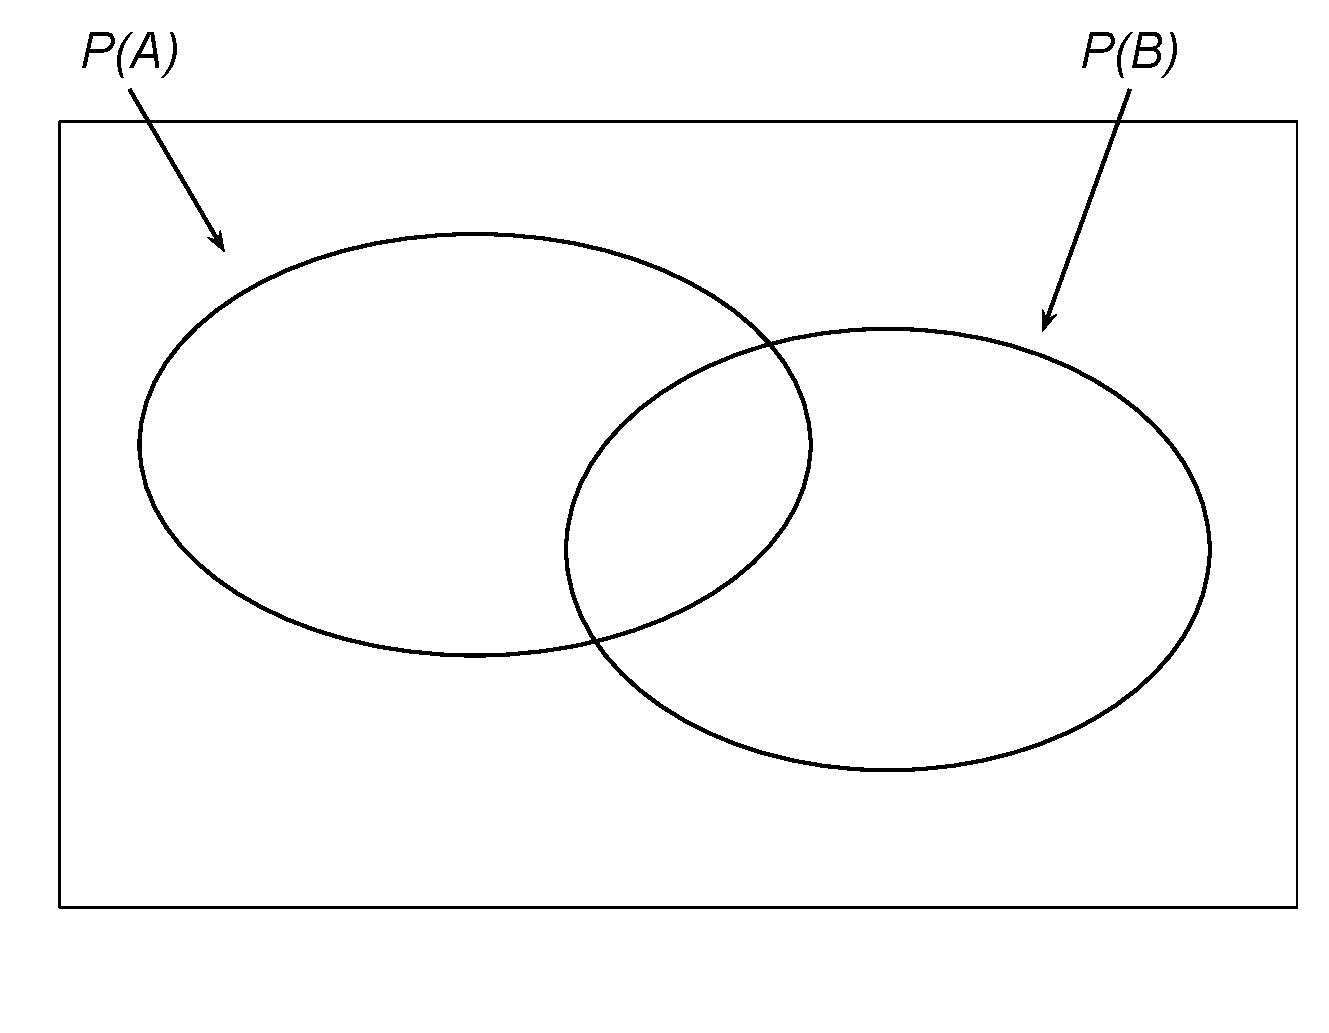
\includegraphics[width=6cm]{Bayes_Theorem_Example_1.pdf}\end{center}}
\only<5>{\begin{center}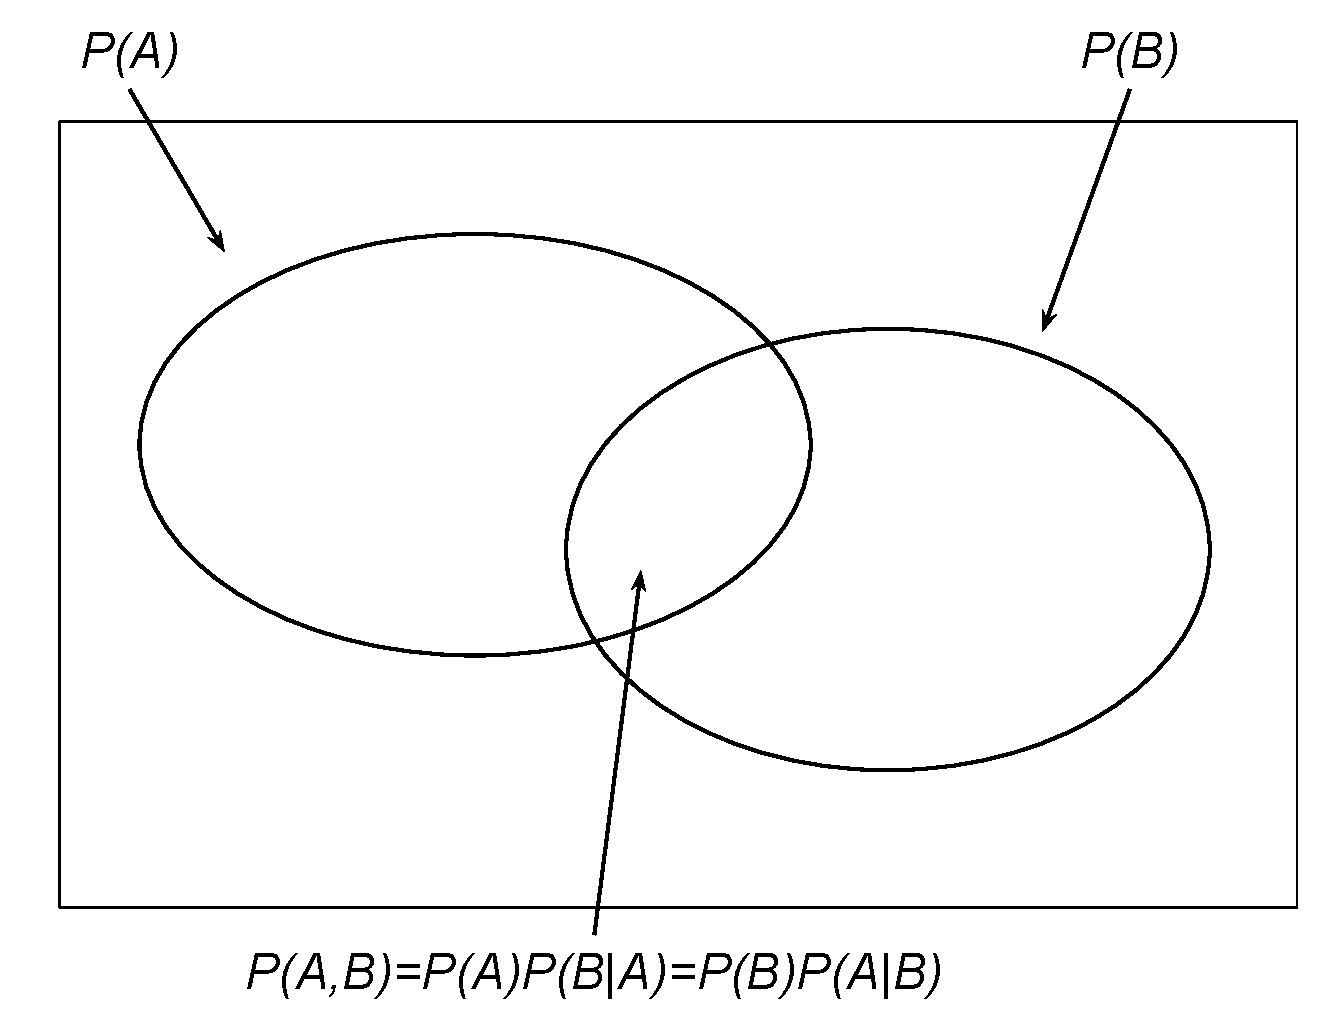
\includegraphics[width=6cm]{Bayes_Theorem_Example.pdf}\end{center}}
}

\frame{\frametitle{Cause of accidents}

Consider the following two events:
\begin{itemize}
\item $A$: There is an obstacle on the road.
\item $B$: I have an accident.
\end{itemize}
Let $P(A)=.3$, $P(B)=.5$ and $P(B|A)={2\over3}$.\vspace{.5cm}

If I've had an accident what is the chance that it was caused by an obstacle on the road?
$$P(A)P(B|A)=P(B)P(A|B)$$
$$\Leftrightarrow$$
$$P(A|B)={P(A)P(B|A)\over P(B)}={.3{2\over3}\over.5}={2\over5}$$
}


\frame{\frametitle{Bayes' Theorem}
The difficulty of decision making lies with the ``uncertainty of state''. Very often experiments can be done to improve our prior estimates of the probabilities of each state. The improved estimates are called \emph{posterior probabilities}. A useful tool for calculating posterior probabilities is \emph{Bayes' Theorem}:
\begin{theorem}
Suppose that $A_1,A_2,\dots,A_n$ are mutually exclusive events and the union of these events is the entire sample space, then for any other event $B$,
$$\begin{array}{@{}r@{\;}c@{\;}l@{}}P(A_i\;|\;B)&=&{P(A_i)P(B\;|\;A_i)\over P(B)}\\[2mm]&=&{P(A_i)P(B\;|\;A_i)\over P(A_1)P(B\;|\;A_1)+\dots+P(A_n)P(B\;|\;A_n)}\end{array}$$
\end{theorem}
}

\frame{\frametitle{Example}
In a nuclear plant, there are 3 main causes of accidents:
\begin{itemize}
\item Human error (H):
$$P(H)=.02,\;P(E\;|\;H)=.01$$
\item Mechanical error (M):
$$P(M)=.01,\;P(E\;|\;M)=.05$$
\item Natural disaster (D):
$$P(D)=.001,\;P(E\;|\;D)=.1$$
\end{itemize}
The nuclear plant has exploded. What is the probability that it is due to a mechanical error?}

\frame{\frametitle{Solution}
Recall:
$$P(H)=.02,\;P(M)=.01,\;P(D)=.001$$
and
$$P(E\;|\;H)=.01,\;P(E\;|\;M)=.05,\;P(E\;|\;D)=.1$$
thus:
$$\begin{array}{@{}r@{\;}c@{\;}l@{}}P(M\;|\;E)&=&{P(M)P(E\;|\;M)\over P(H)P(E\;|\;H)+P(M)P(E\;|\;M)+P(D)P(E\;|\;D)}\\[2mm]&=&{.05\times.01\over .01\times.02+.05\times.01+.1\times.001}\end{array}$$
}

\frame{\frametitle{Decision Trees}Decision trees are used to calculate expected payoffs for different decisions. We will illustrate this with the following problem. A company is considering an investment in a certain stock. The company assesses that the stock has a $60\%$ chance of going up, in which case they can make a profit of 20. If the stock goes down they will lose 20.\\\vspace{.5cm}

The company has the option of paying a financial advisor $C$ thousand for an assessment of the stock (we will allow $C$ to vary). The advisor is known to be $80\%$ successful at forecasting a stock increase and $70\%$ successful at forecasting a stock decrease. We will draw the decision tree for this problem and describe how it is constructed.
}

\frame{\frametitle{Step 1: Set out Decisions and Variable outcomes}
Firstly we set out the possible decisions and variable outcomes. Decisions are denoted by square boxes and variable outcomes by circles.
}

\frame{\frametitle{Step 1: Set out Decisions and Variable outcomes}
\only<1>{\begin{center}
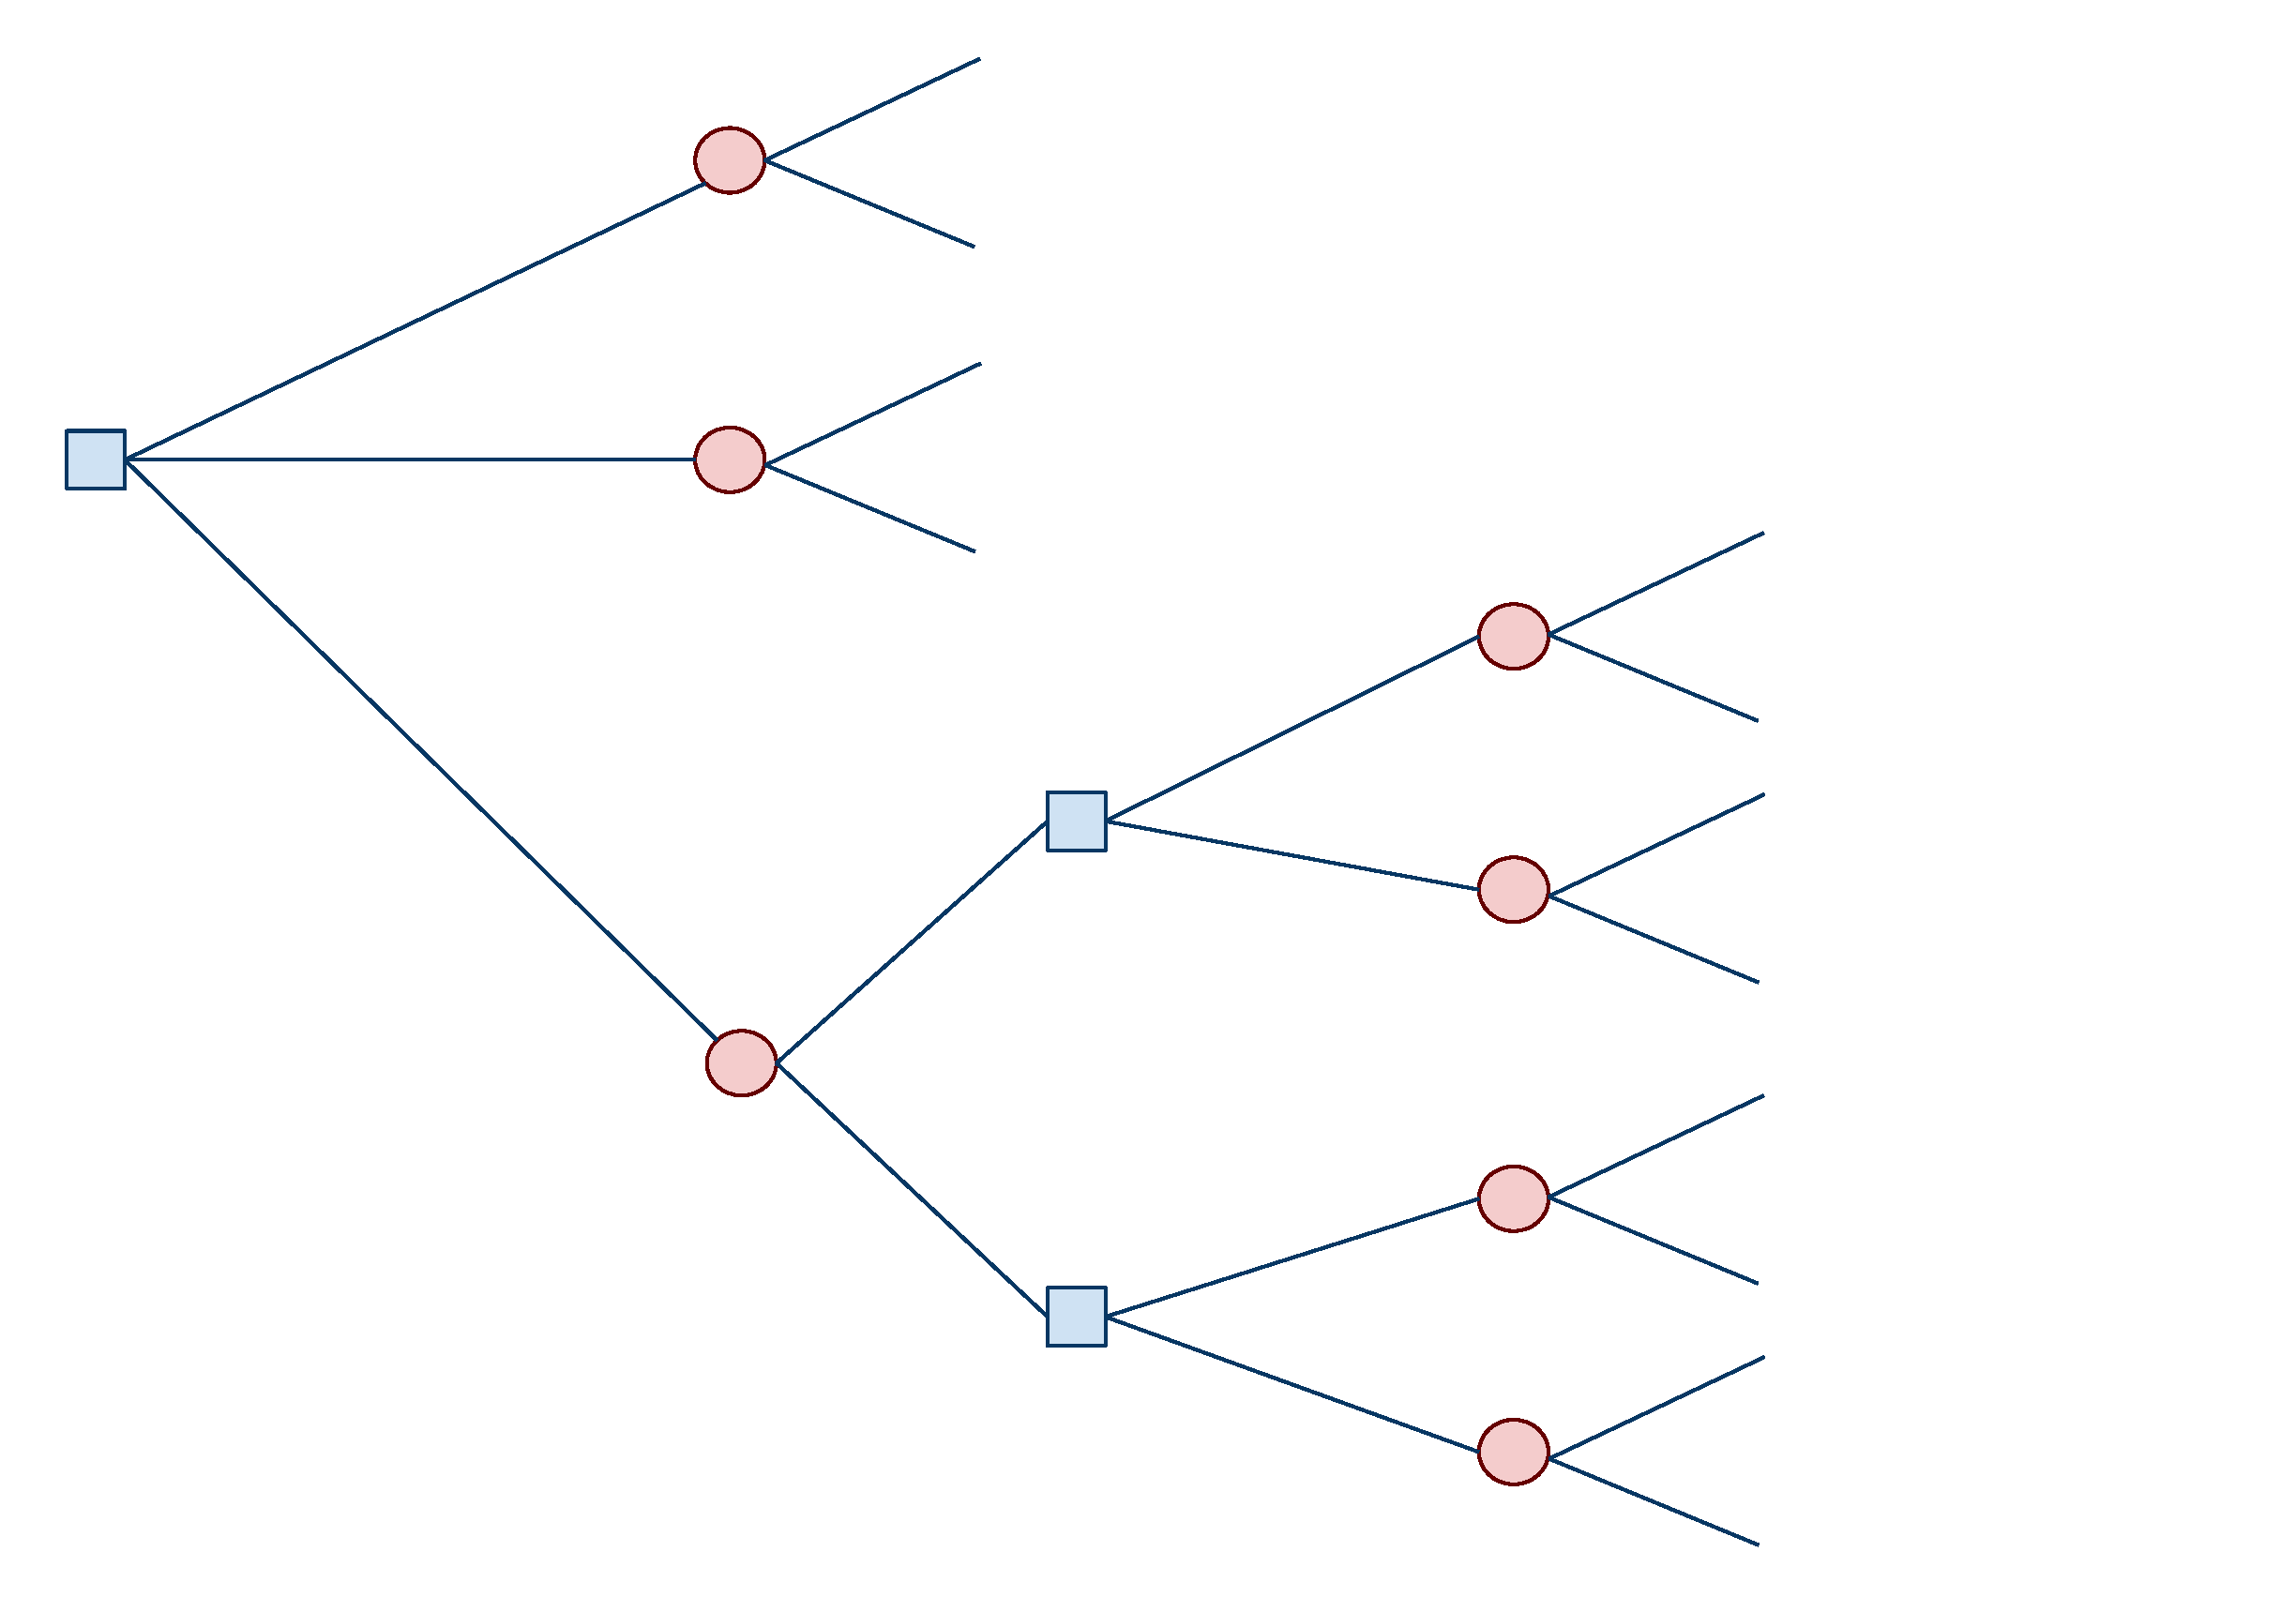
\includegraphics[width=10cm]{Stock_Example_Decision_Tree_1.pdf}
\end{center}}
\only<2>{\begin{center}
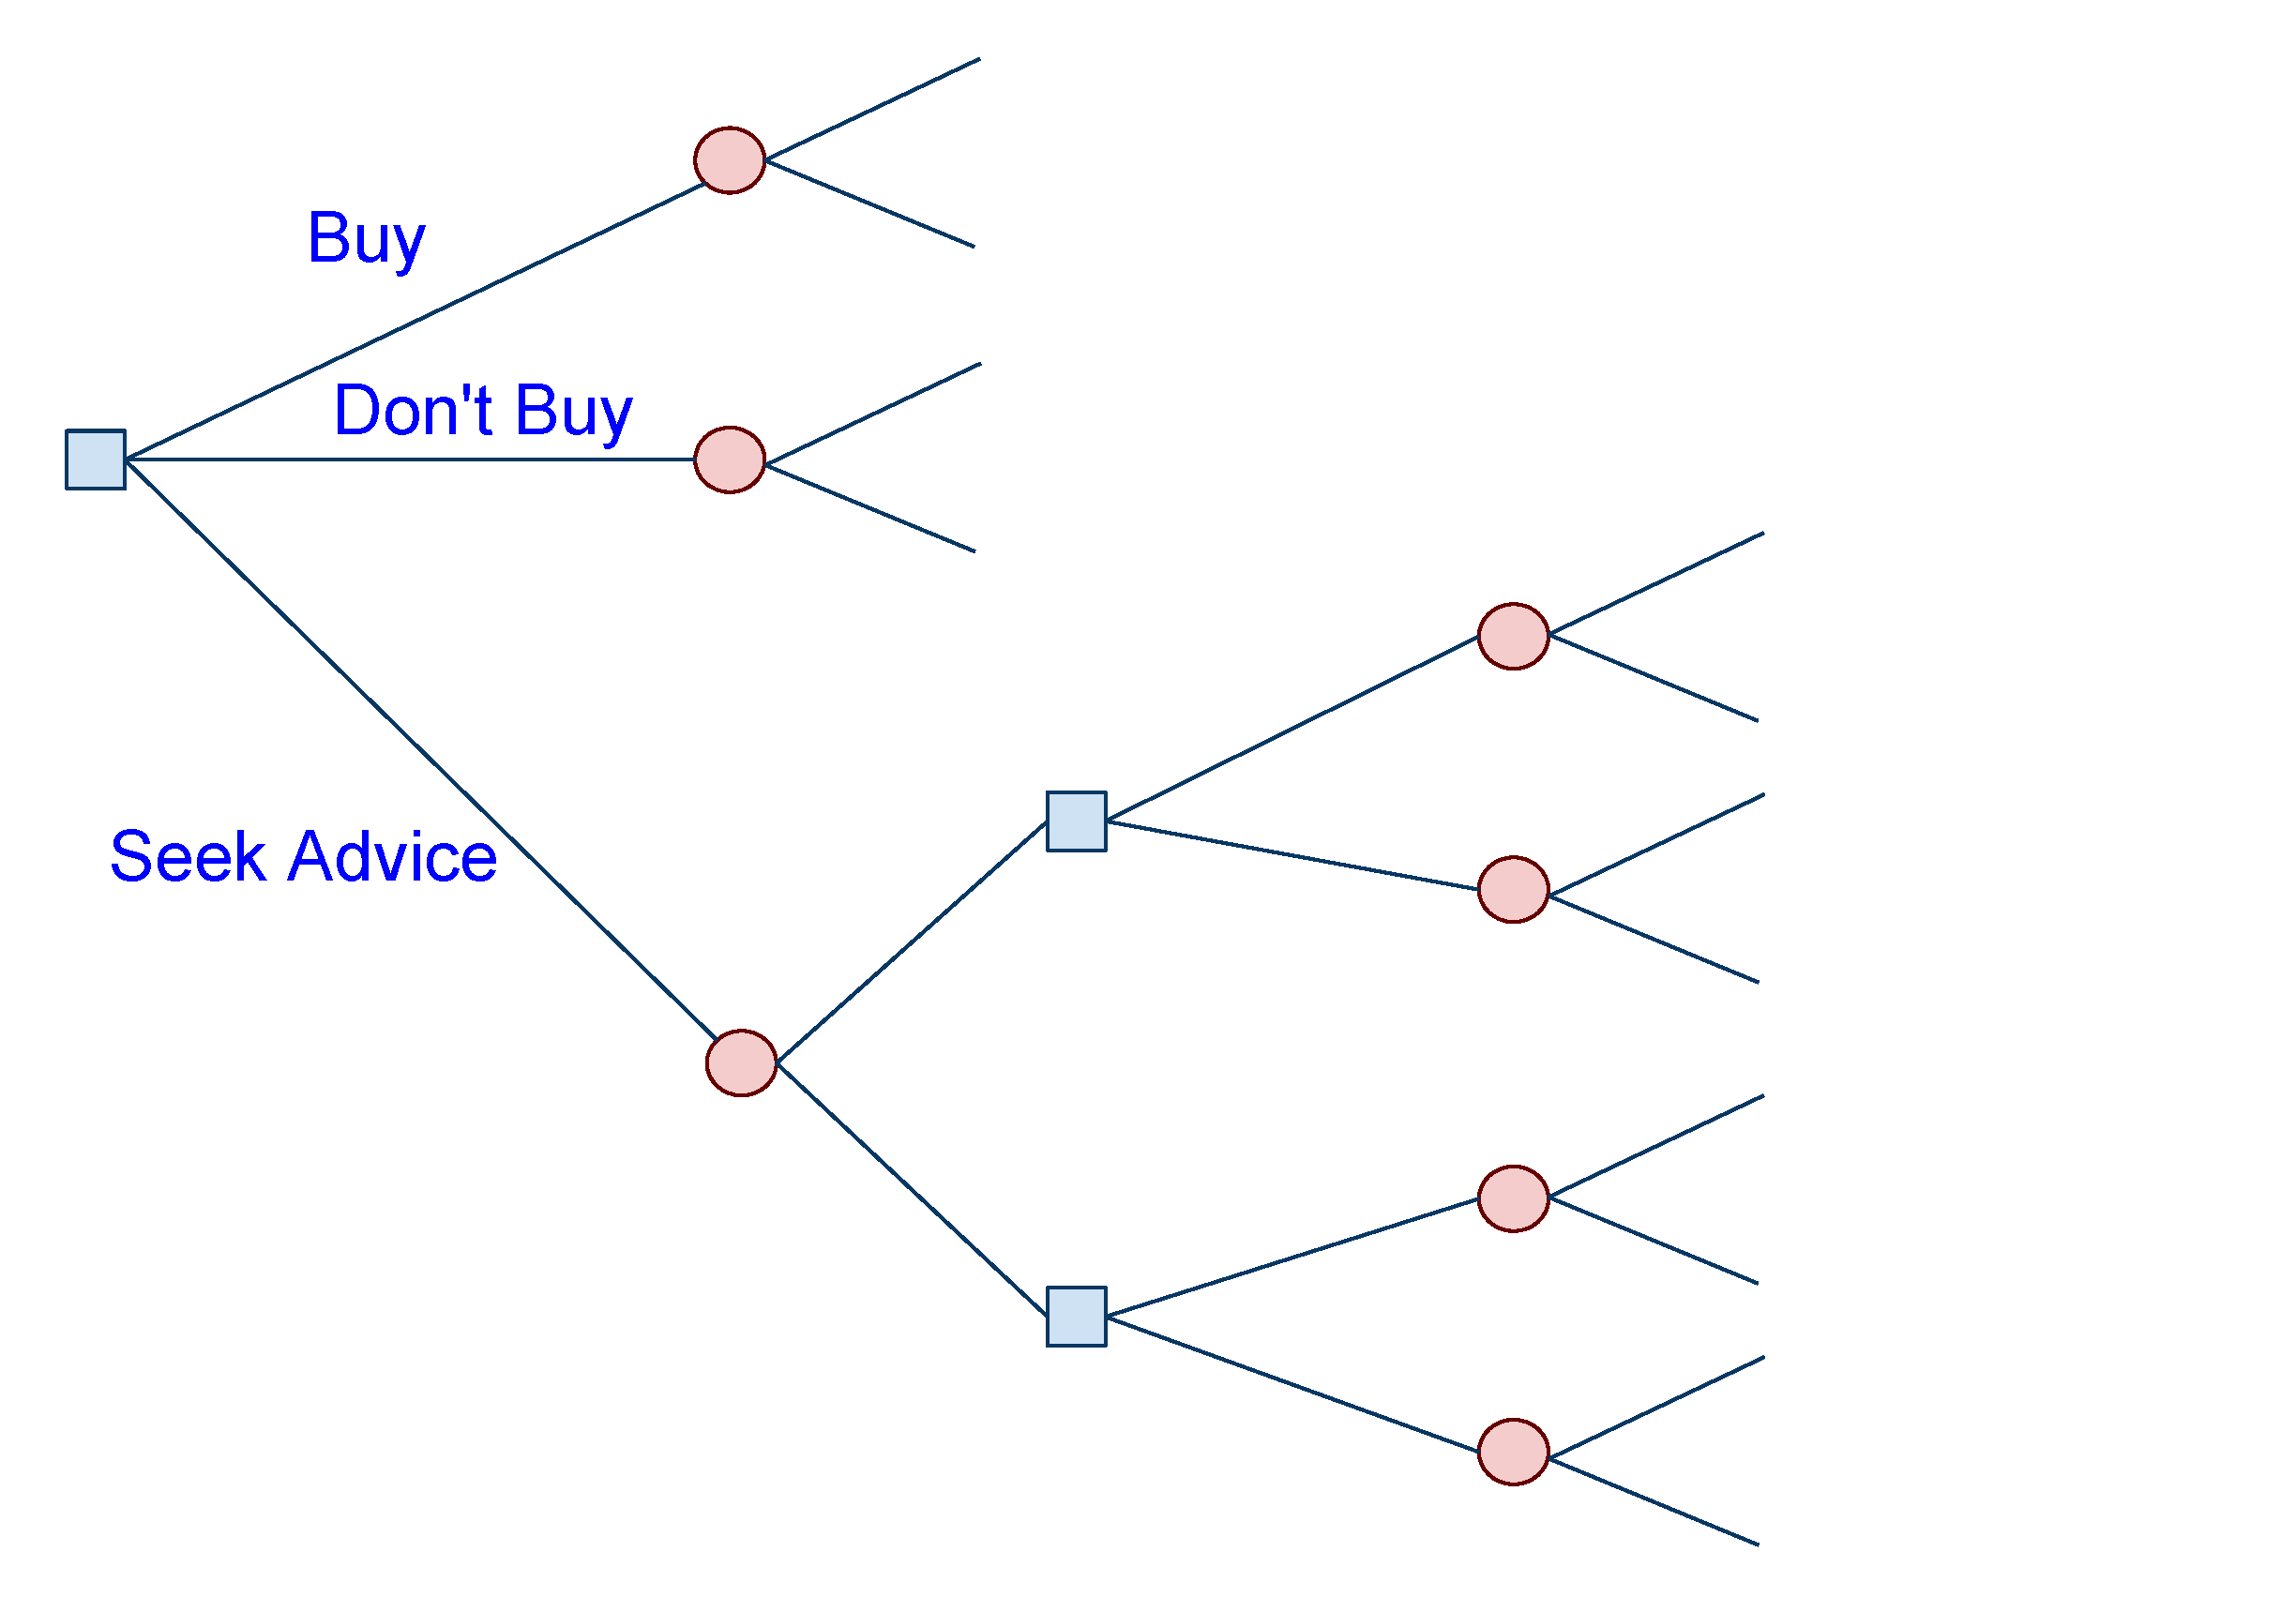
\includegraphics[width=10cm]{Stock_Example_Decision_Tree_2.pdf}
\end{center}}
\only<3>{\begin{center}
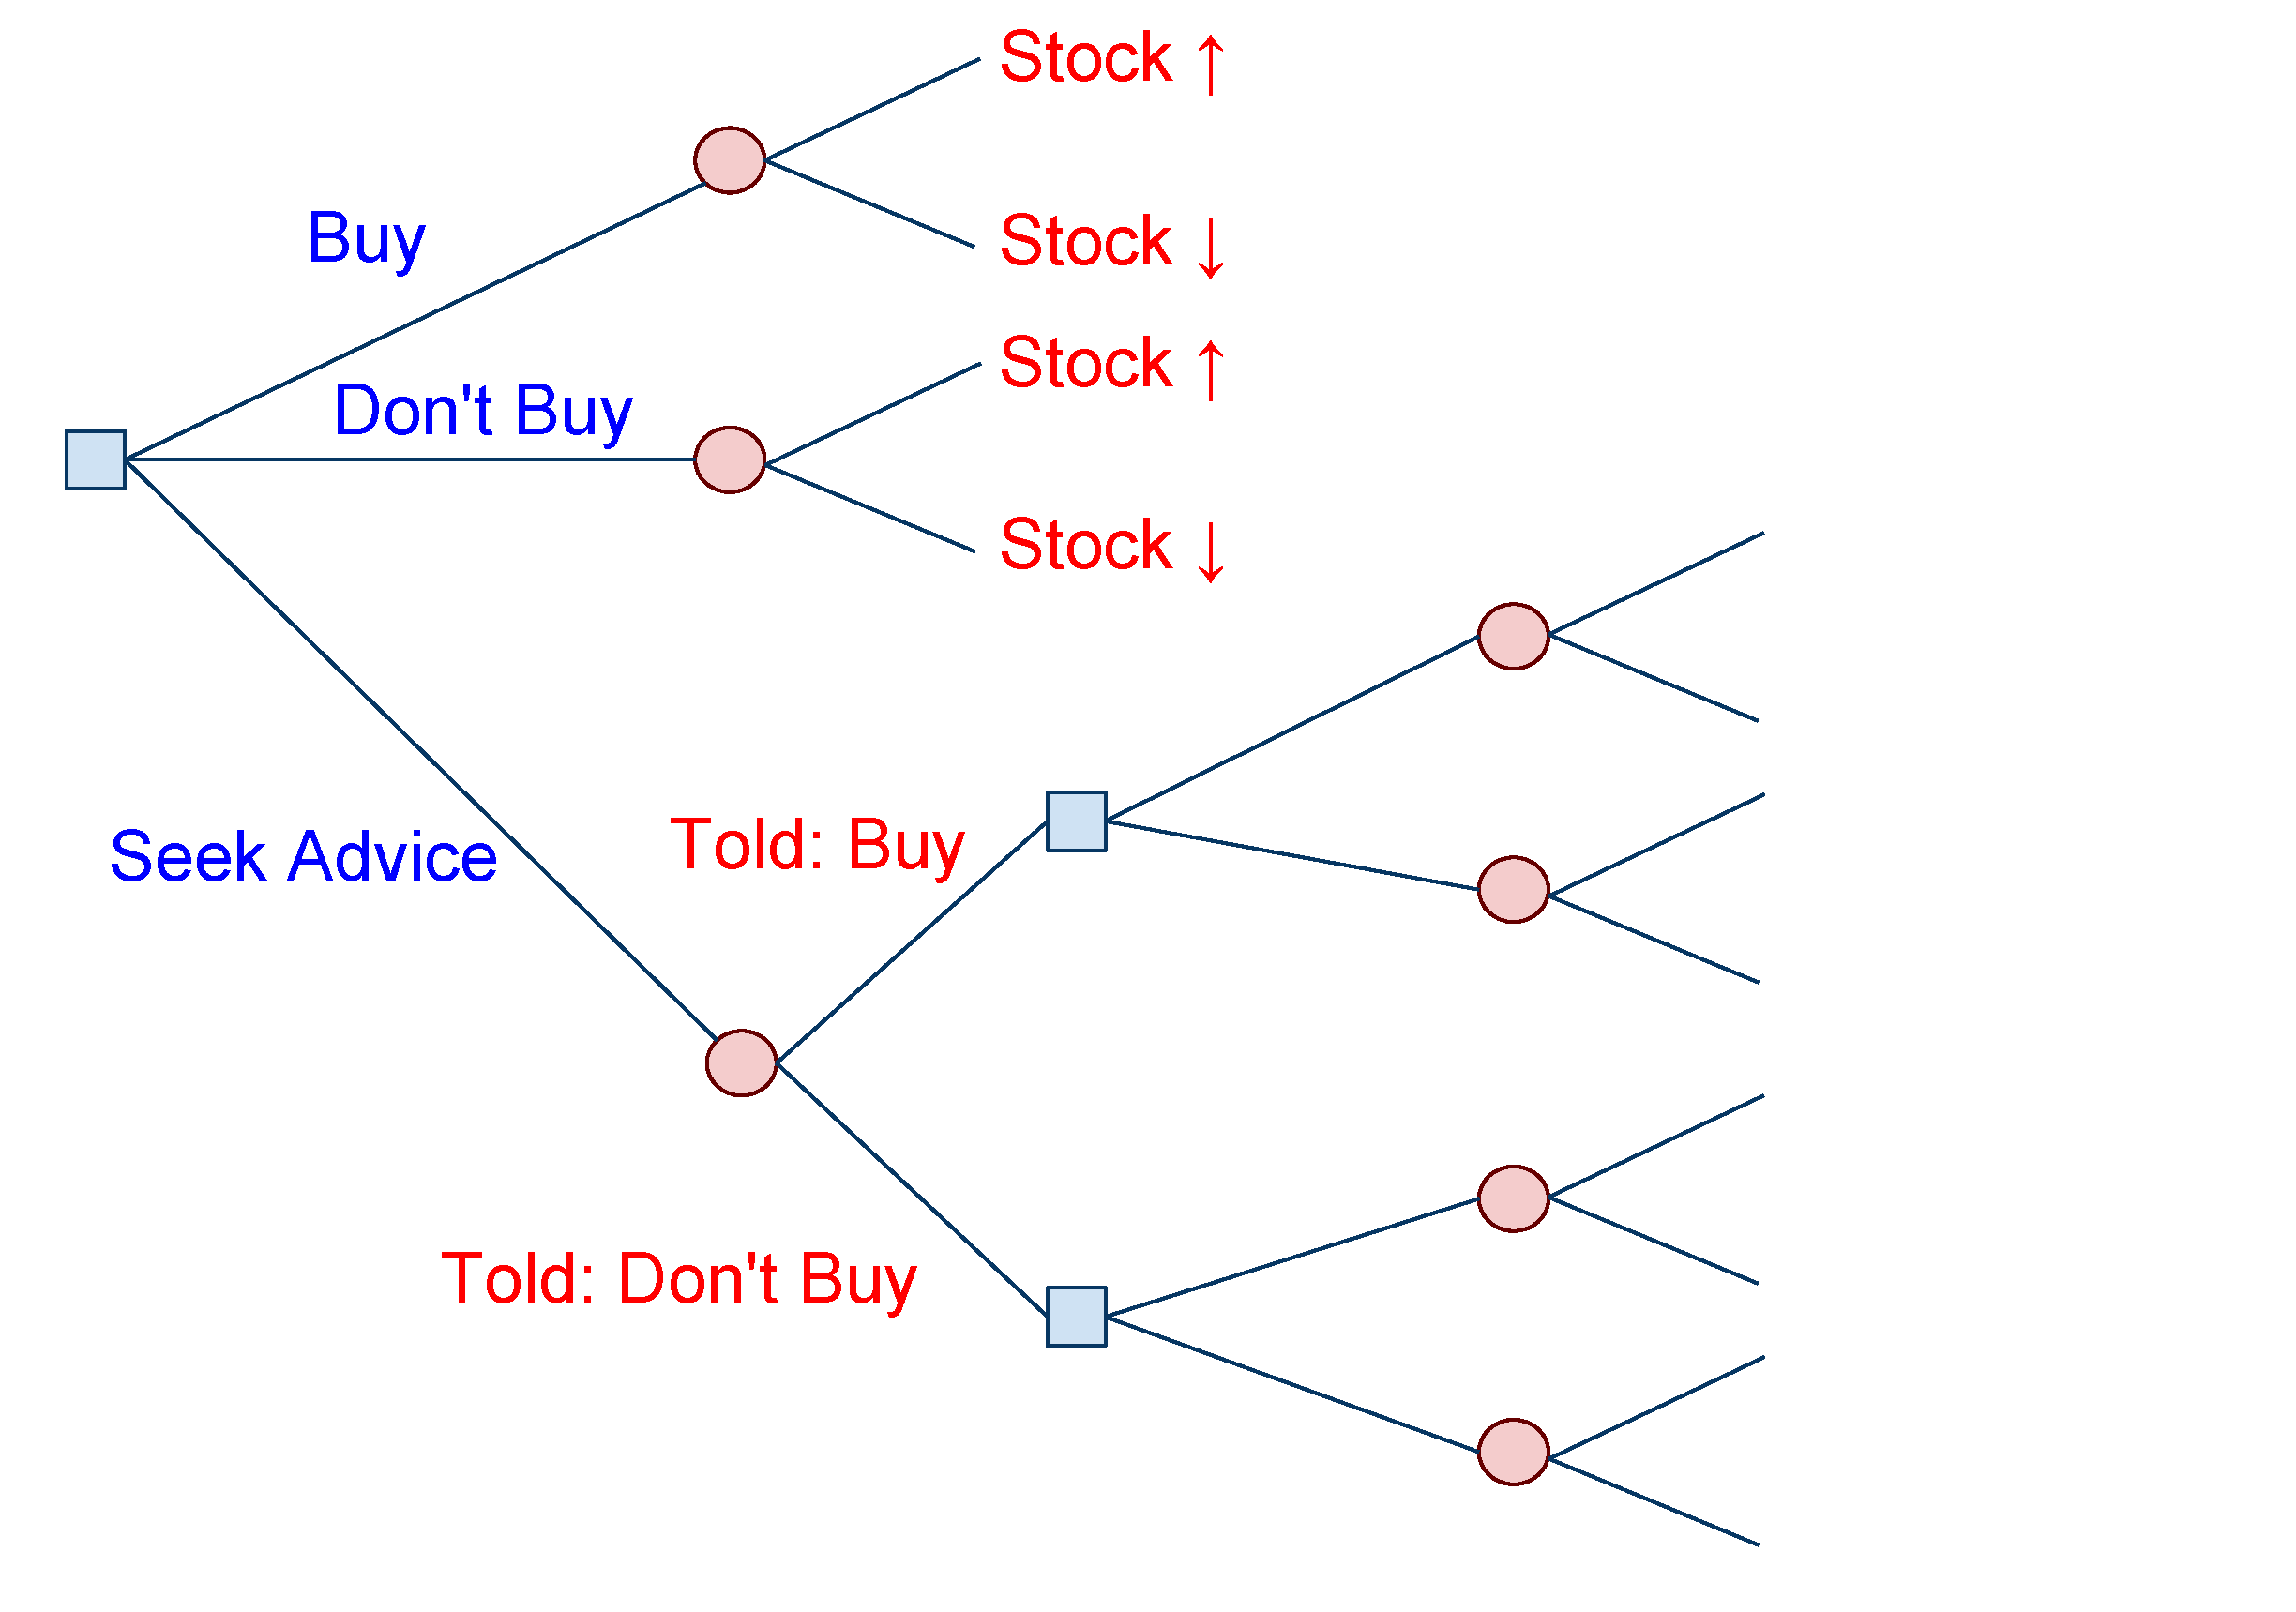
\includegraphics[width=10cm]{Stock_Example_Decision_Tree_3.pdf}
\end{center}}
\only<4>{\begin{center}
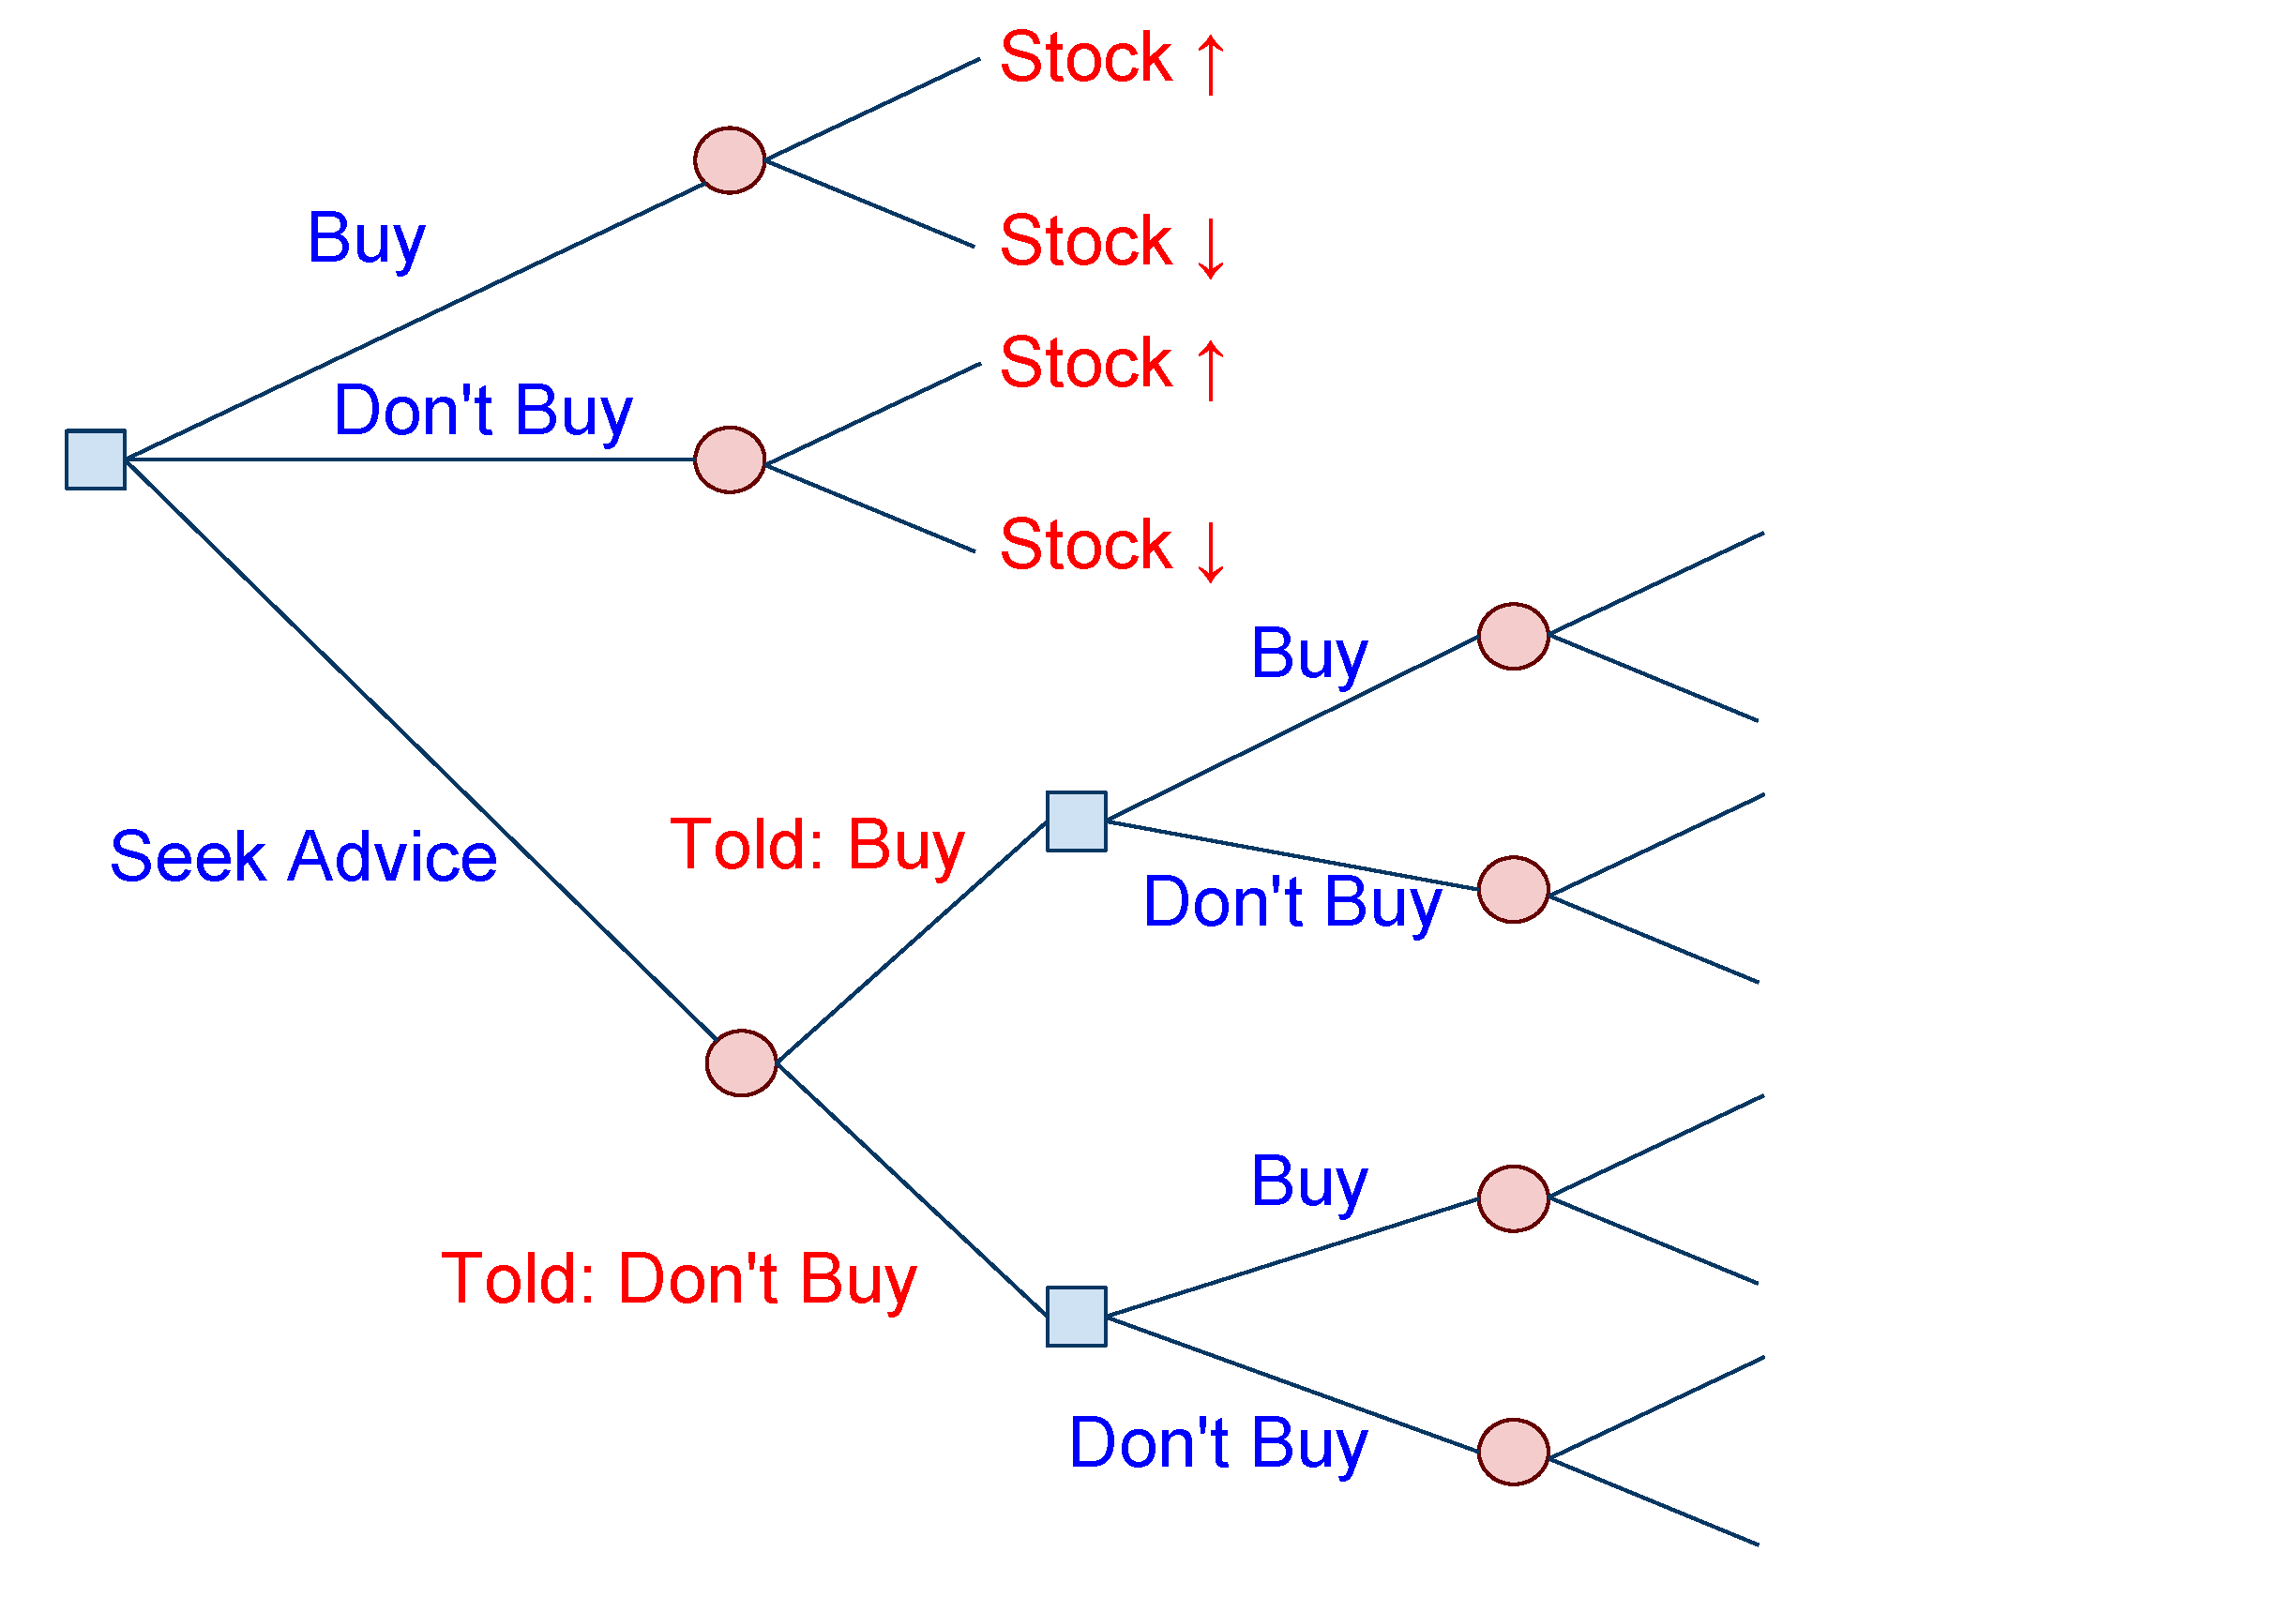
\includegraphics[width=10cm]{Stock_Example_Decision_Tree_4.pdf}
\end{center}}
\only<5>{\begin{center}
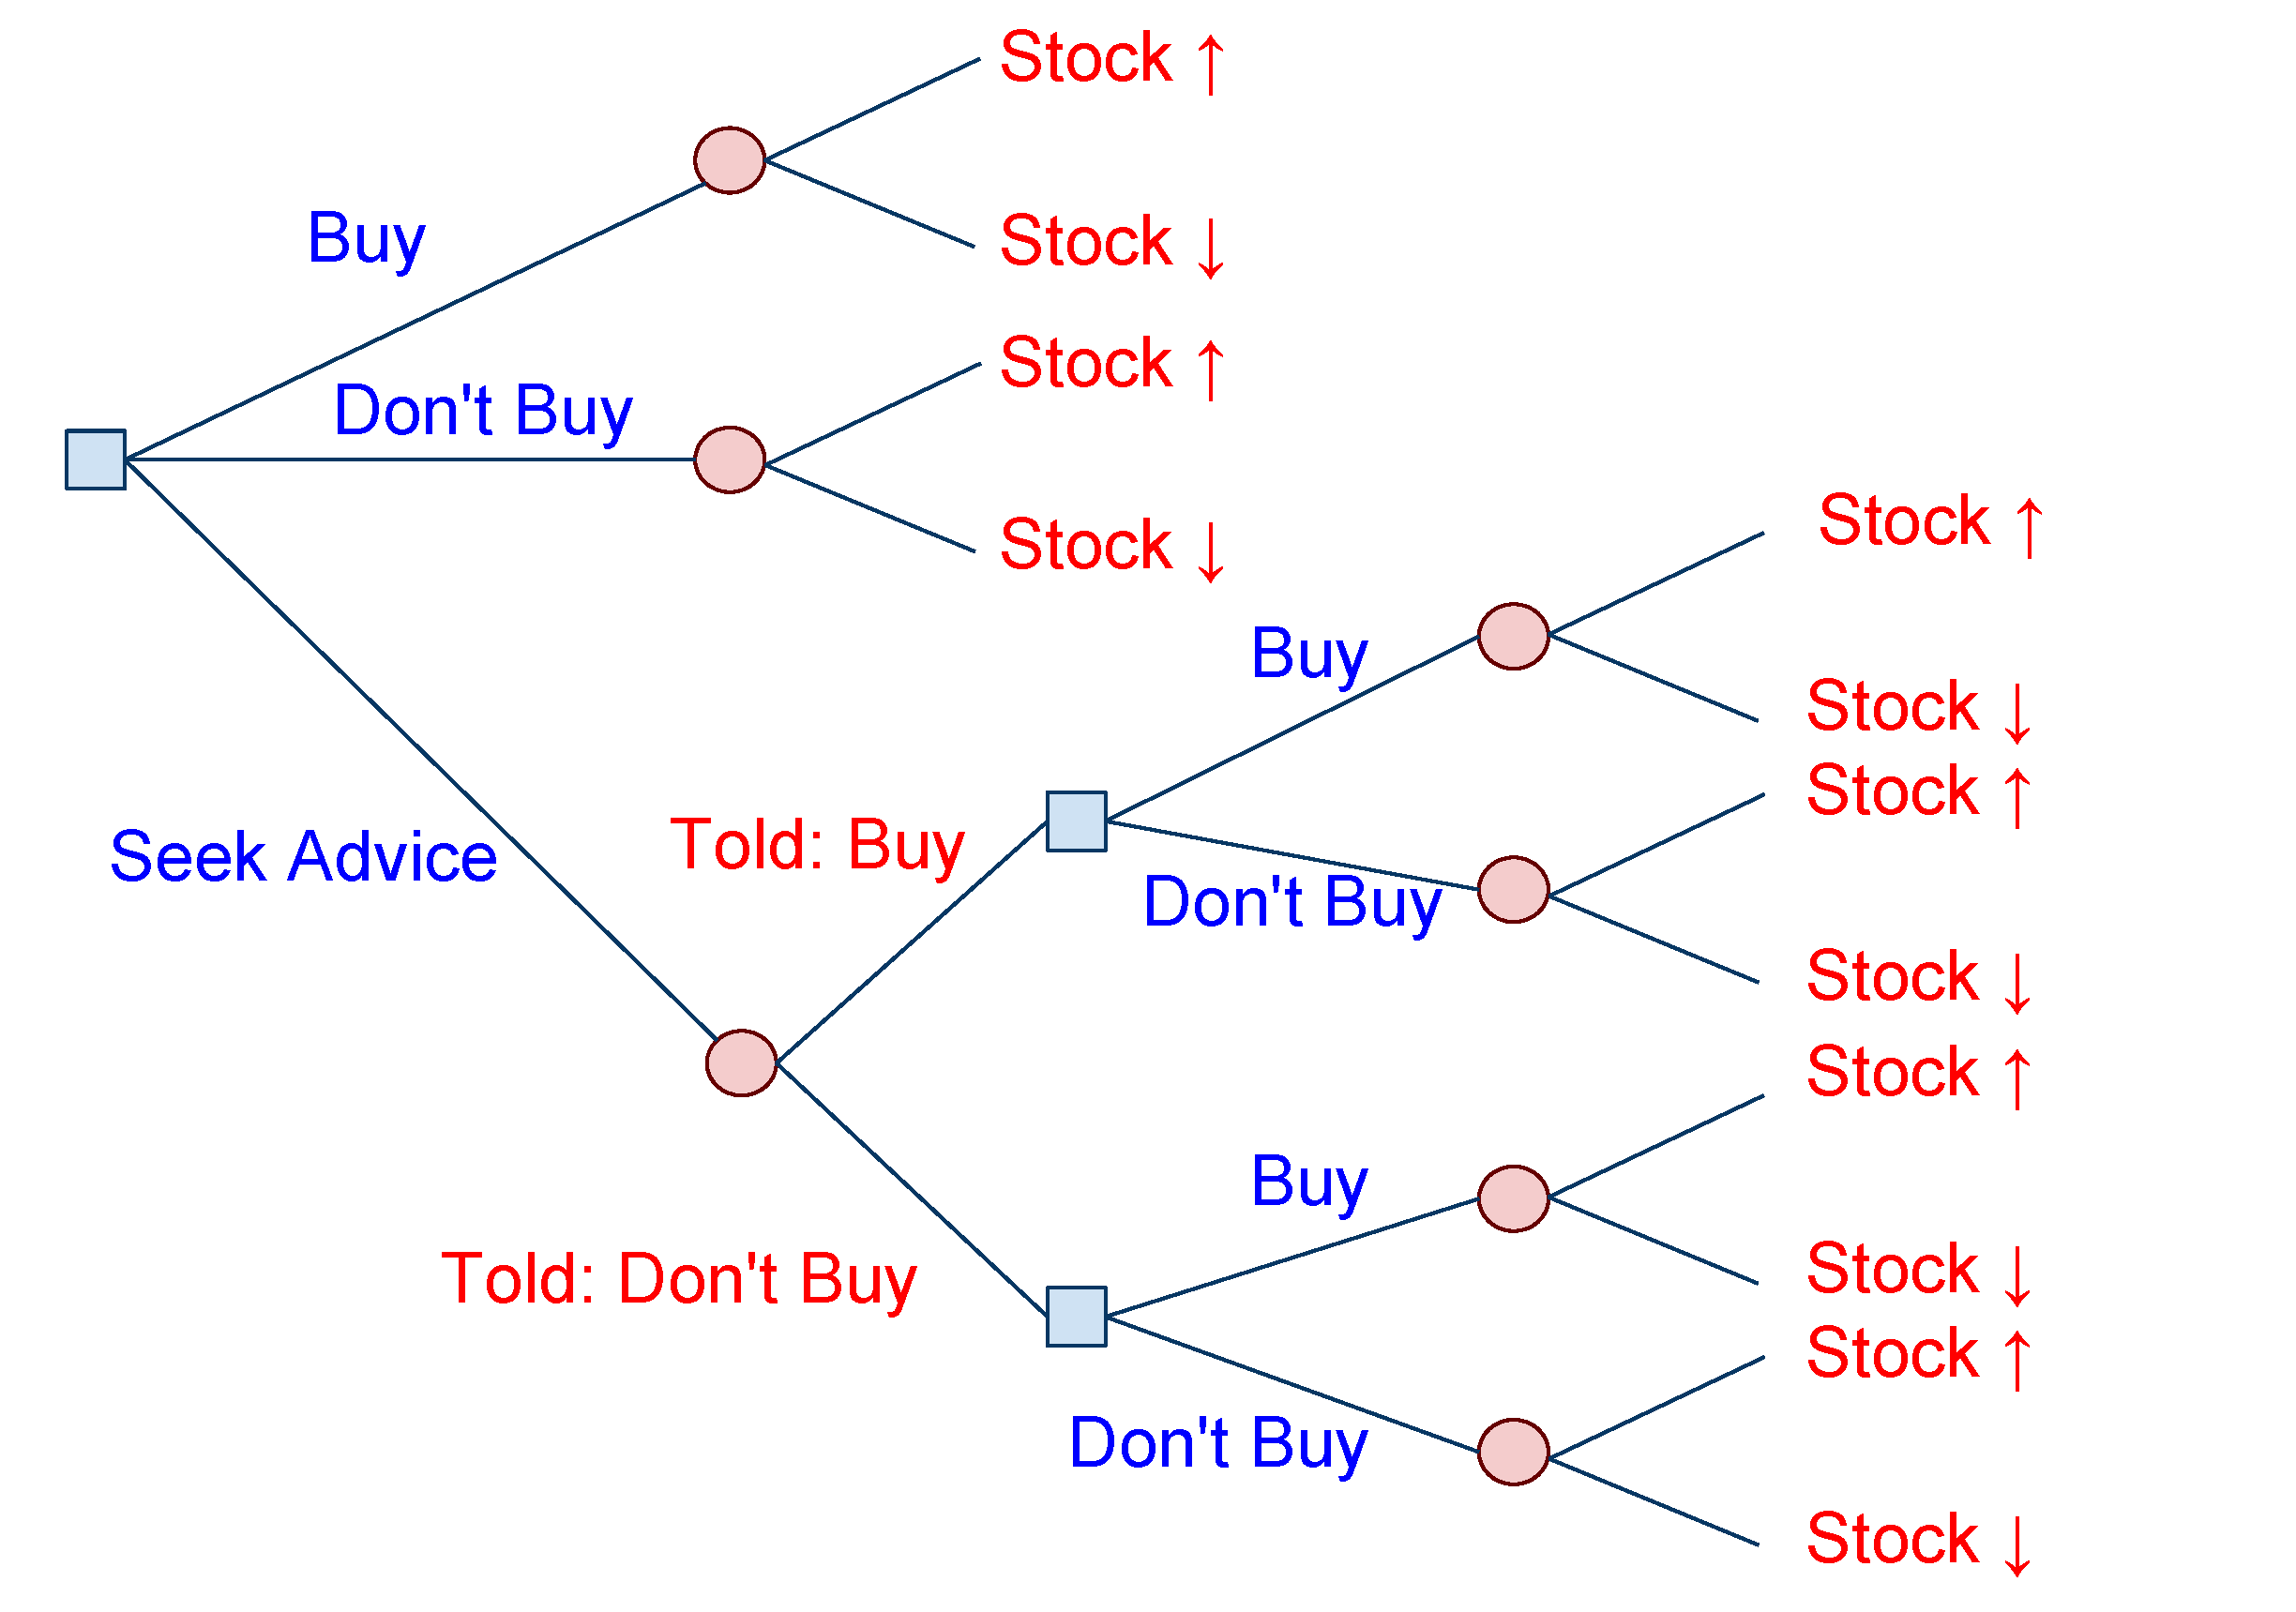
\includegraphics[width=10cm]{Stock_Example_Decision_Tree_5.pdf}
\end{center}}


}

\frame{\frametitle{Step 2: Calculate the Returns}
Next we work out the return for each possible combination of decisions and outcomes.
}

\frame{\frametitle{Step 2: Calculate the Returns}
\only<1>{\begin{center}
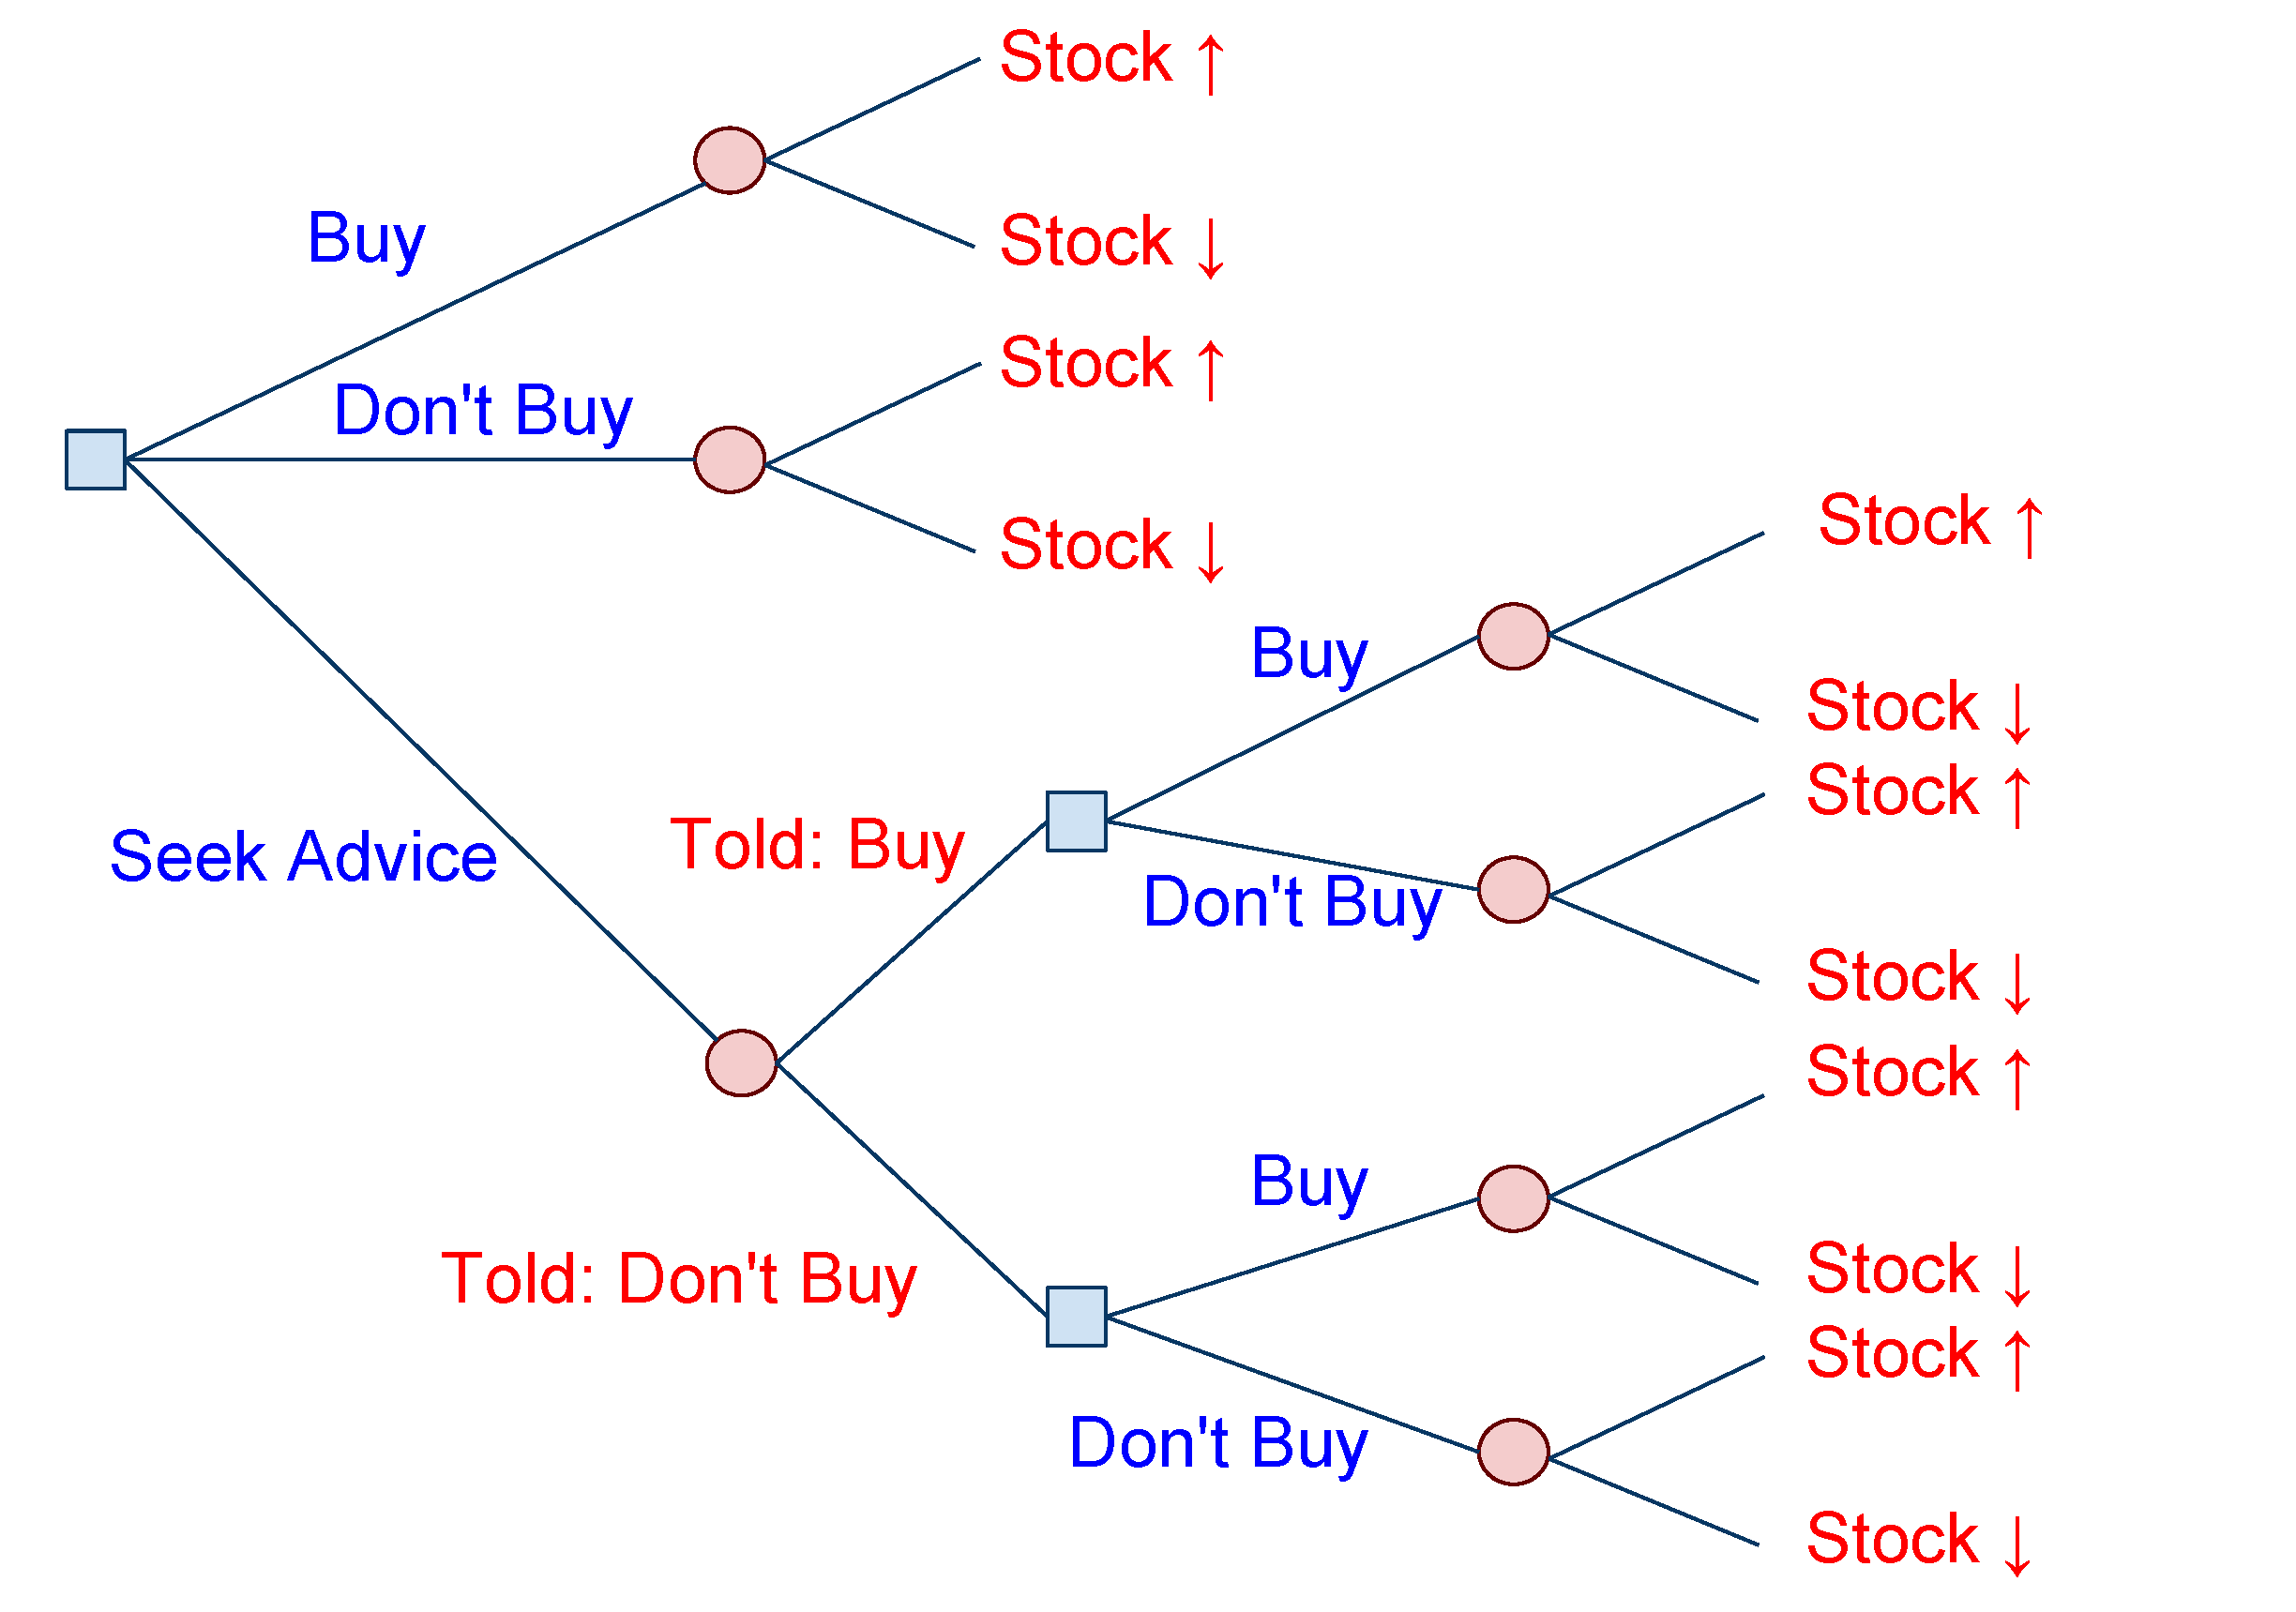
\includegraphics[width=10cm]{Stock_Example_Decision_Tree_5.pdf}
\end{center}}
\only<2>{\begin{center}
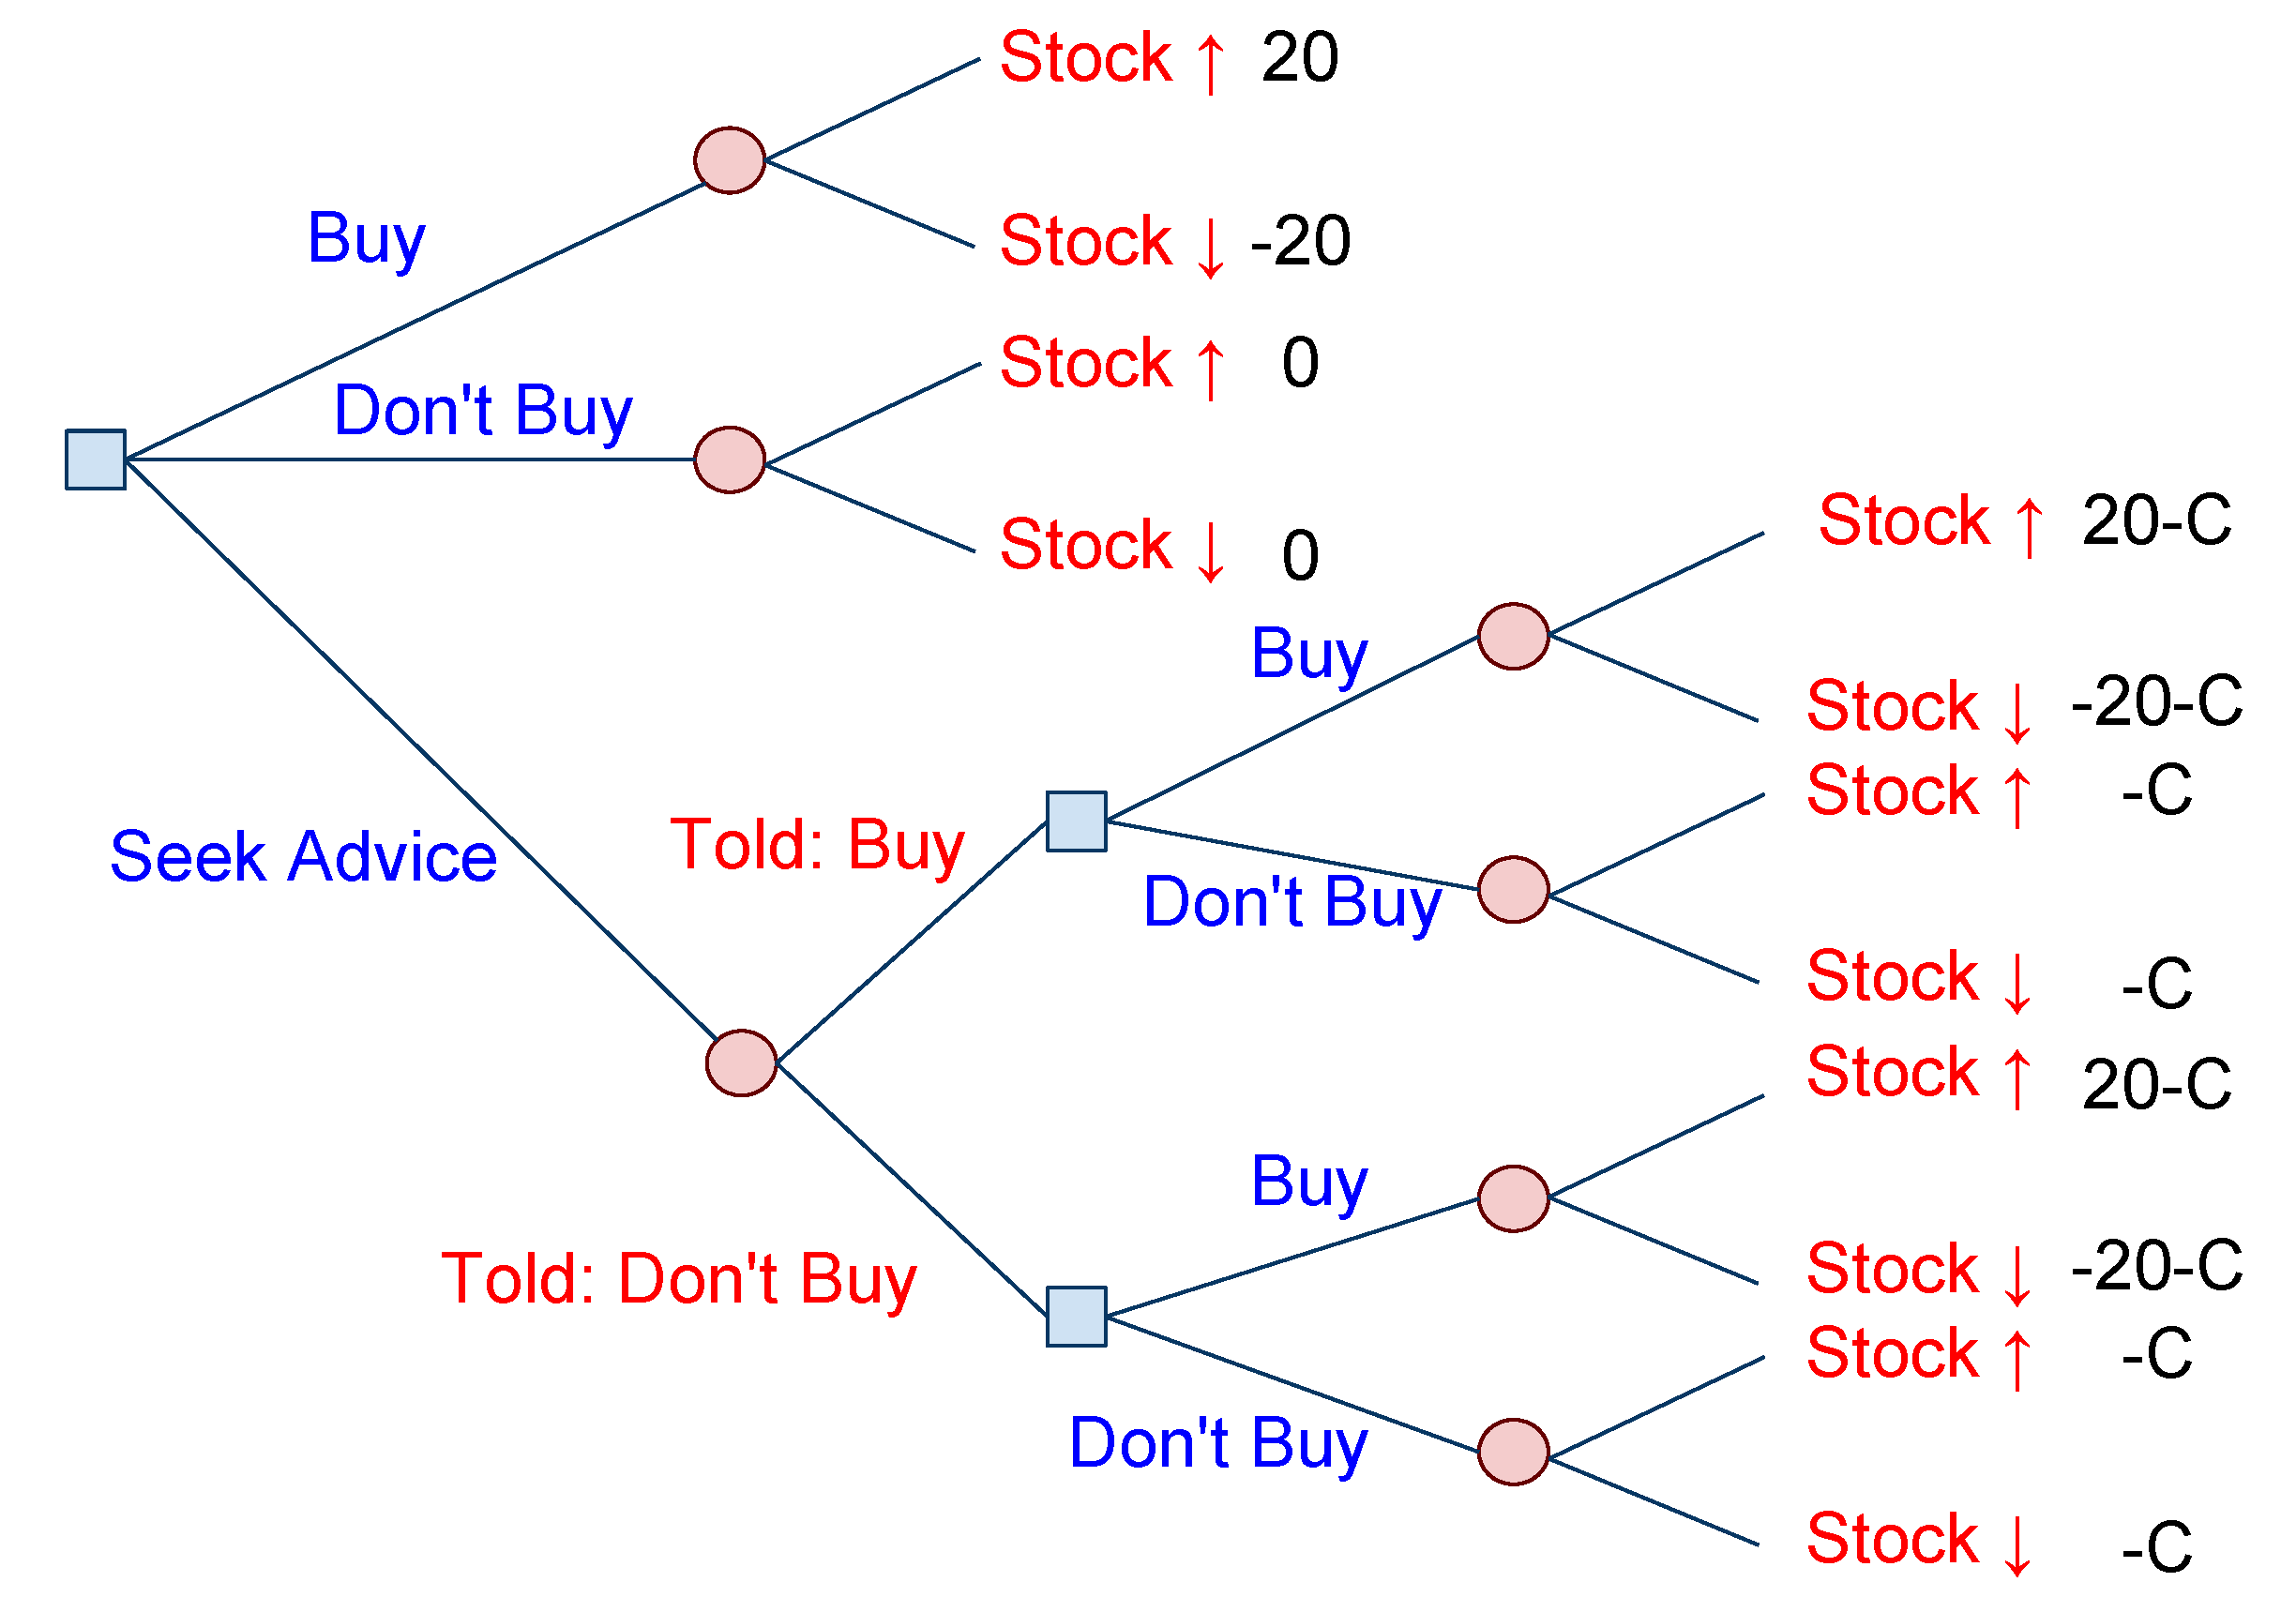
\includegraphics[width=10cm]{Stock_Example_Decision_Tree_6.pdf}
\end{center}}
}

\frame{\frametitle{Step 3: Probabilities of Outcomes}
Next we work out the the probabilities of each variable outcome (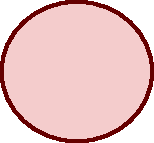
\includegraphics[width=.5cm]{Dot}). This is done from left to right. Note that all probabilities are conditional on outcomes to the left.\\\vspace{.5cm}
Let $U$ be the event \emph{Stock Goes Up}, $D$ the event \emph{Stock Goes Down}, $Y$ the event \emph{Told: Buy} and $N$ the event \emph{Told: Don't Buy}. We have:
$$P(U)=.6,\;P(D)=.4,\;P(Y\;|\;U)=.8\;,P(N\;|\;D)=.7$$
To complete the decision tree we need to know $P(Y),\;P(N),\;P(U\;|\;Y)$ and $P(D\;|\;N)$:
$$\begin{array}{@{}r@{\;}c@{\;}l}P(Y)&=&P(Y\;|\;U)P(U)+P(Y\;|\;D)P(D)=.6\\[2mm]
P(N)&=&1-P(Y)=.4
\end{array}$$
}

\frame{\frametitle{Step 3: Probabilities of Outcomes}
We use Bayes' Theorem to calculate $P(D\;|\;Y)$ and $P(U\;|\;N)$:

$$\begin{array}{@{}r@{\;}c@{\;}l}
P(U\;|\;Y)&=&.8\\[2mm]
P(D\;|\;Y)&=&.2\\[2mm]
P(U\;|\;N)&=&.3\\[2mm]
P(D\;|\;N)&=&.7\\[2mm]
\end{array}$$
}

\frame{\frametitle{Step 3: Probabilities of Outcomes}
\only<1>{\begin{center}
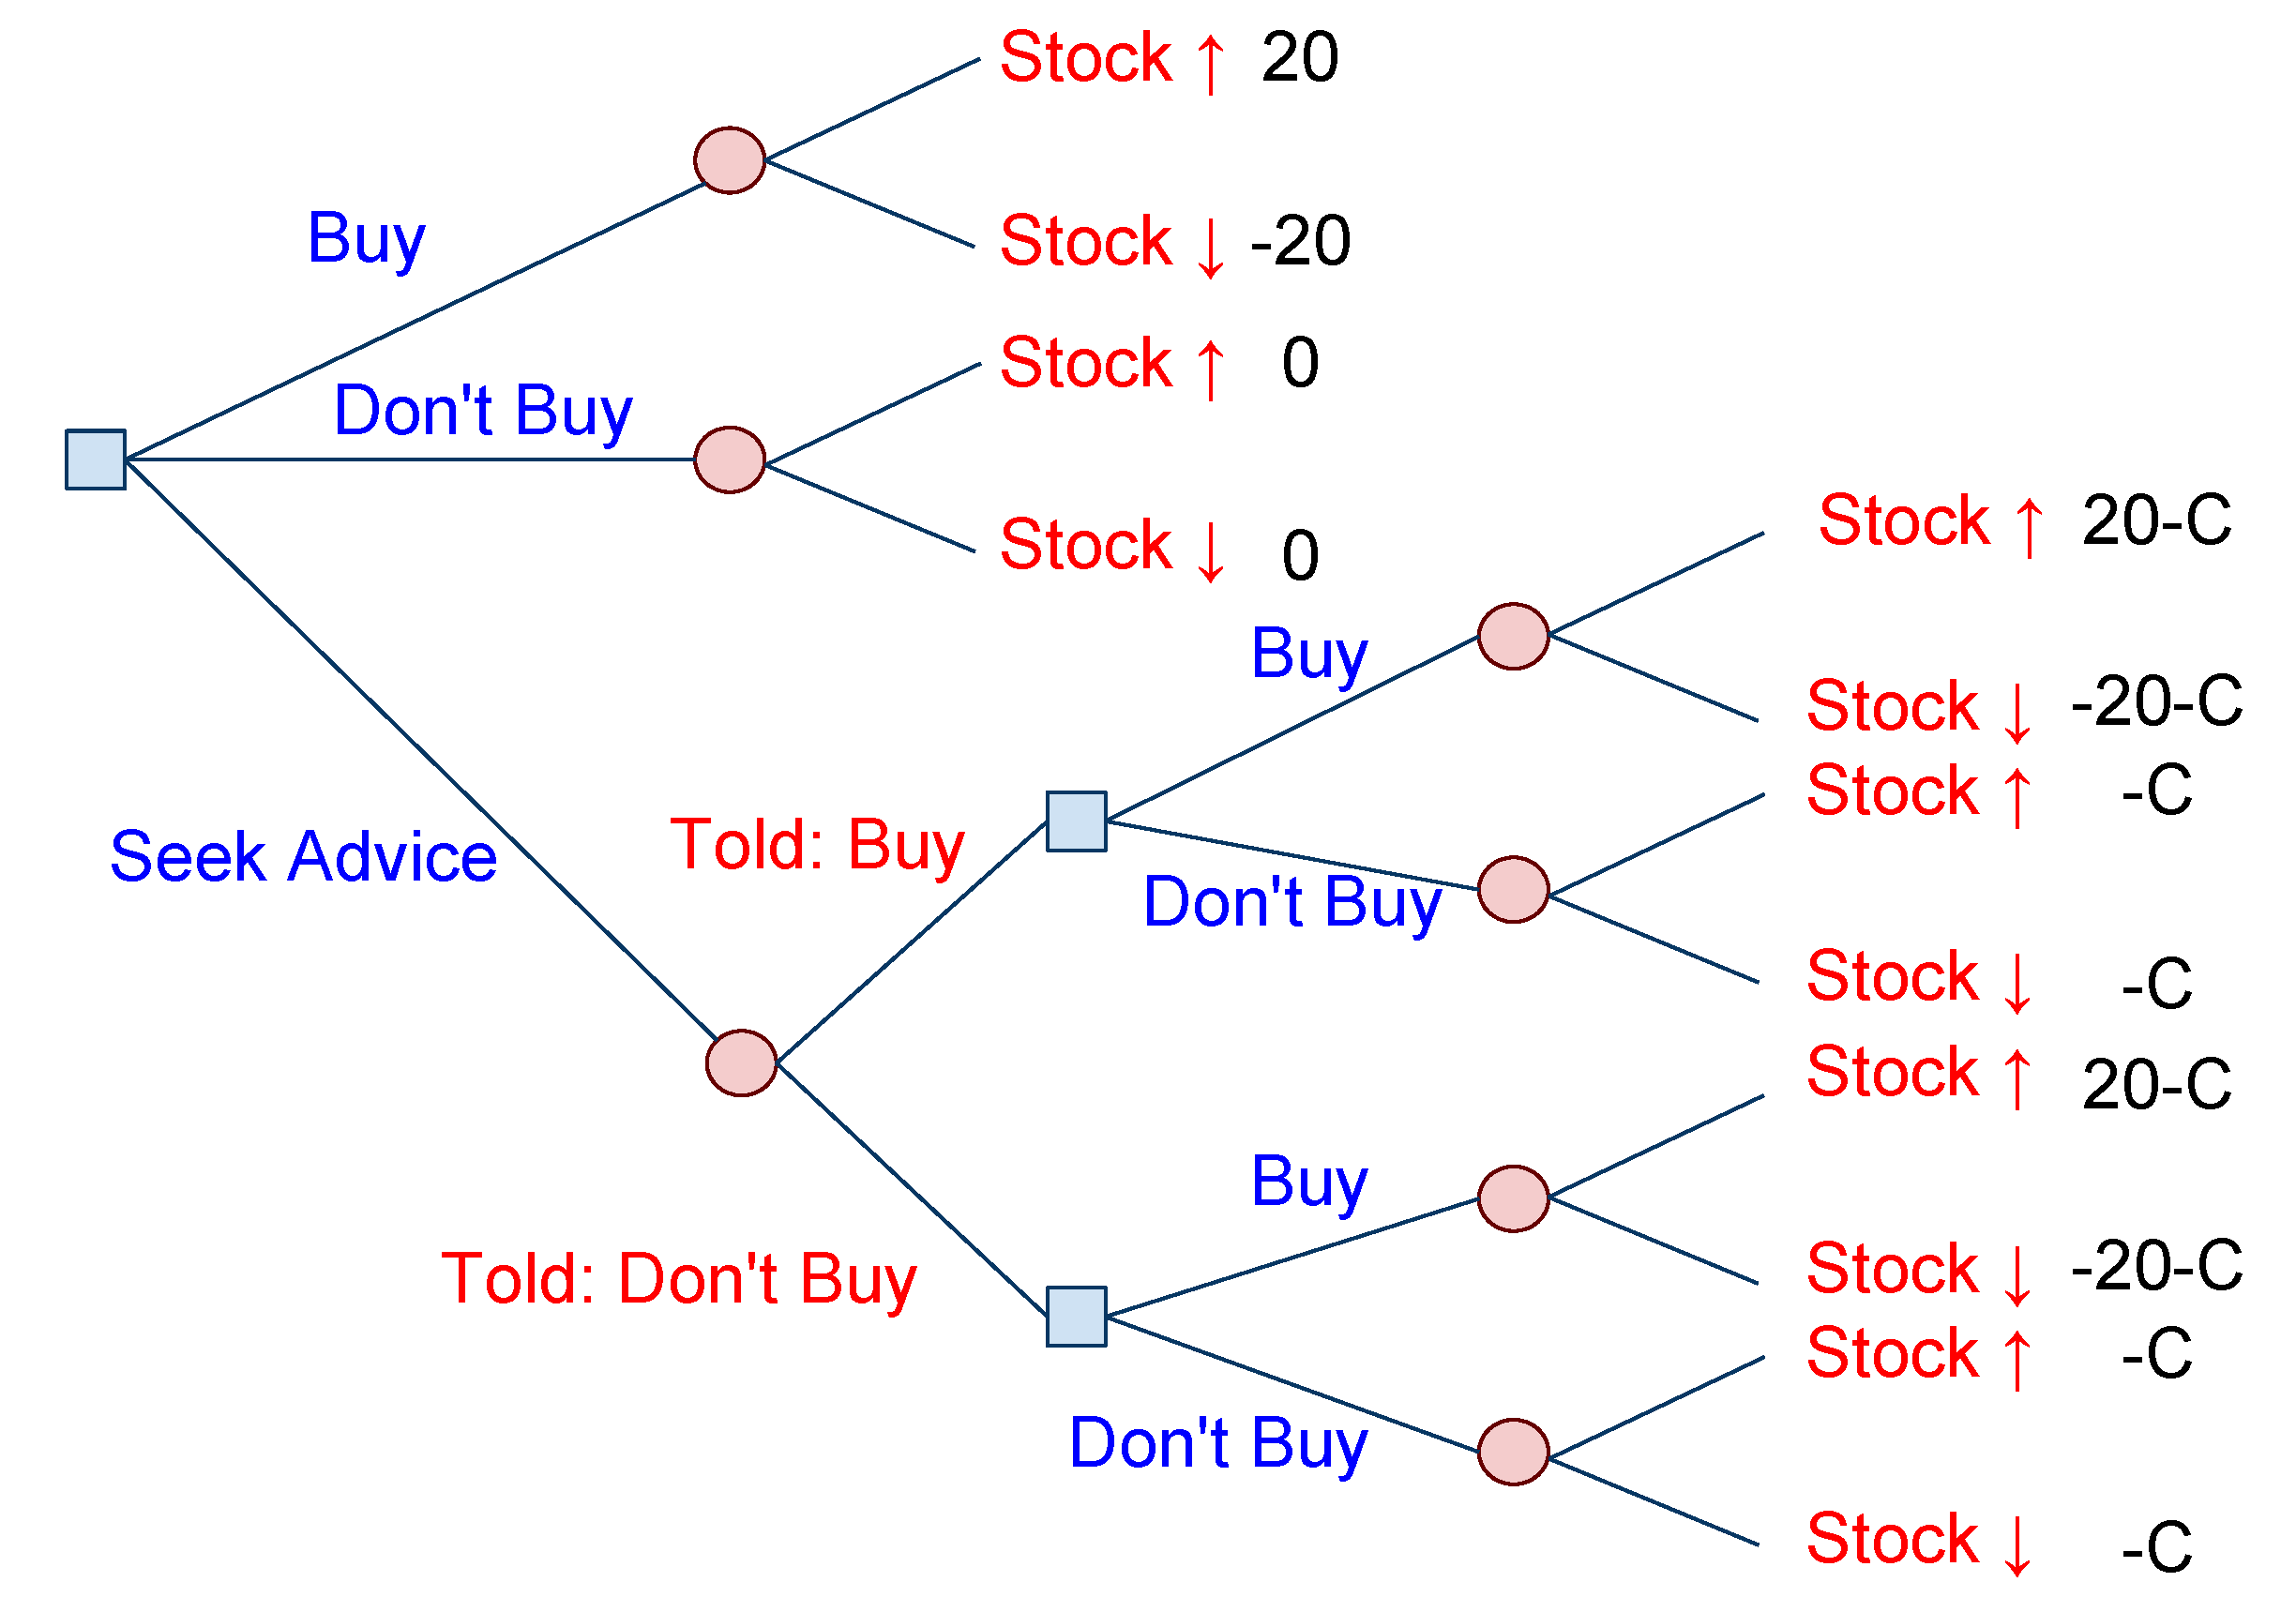
\includegraphics[width=10cm]{Stock_Example_Decision_Tree_6.pdf}
\end{center}}
\only<2>{\begin{center}
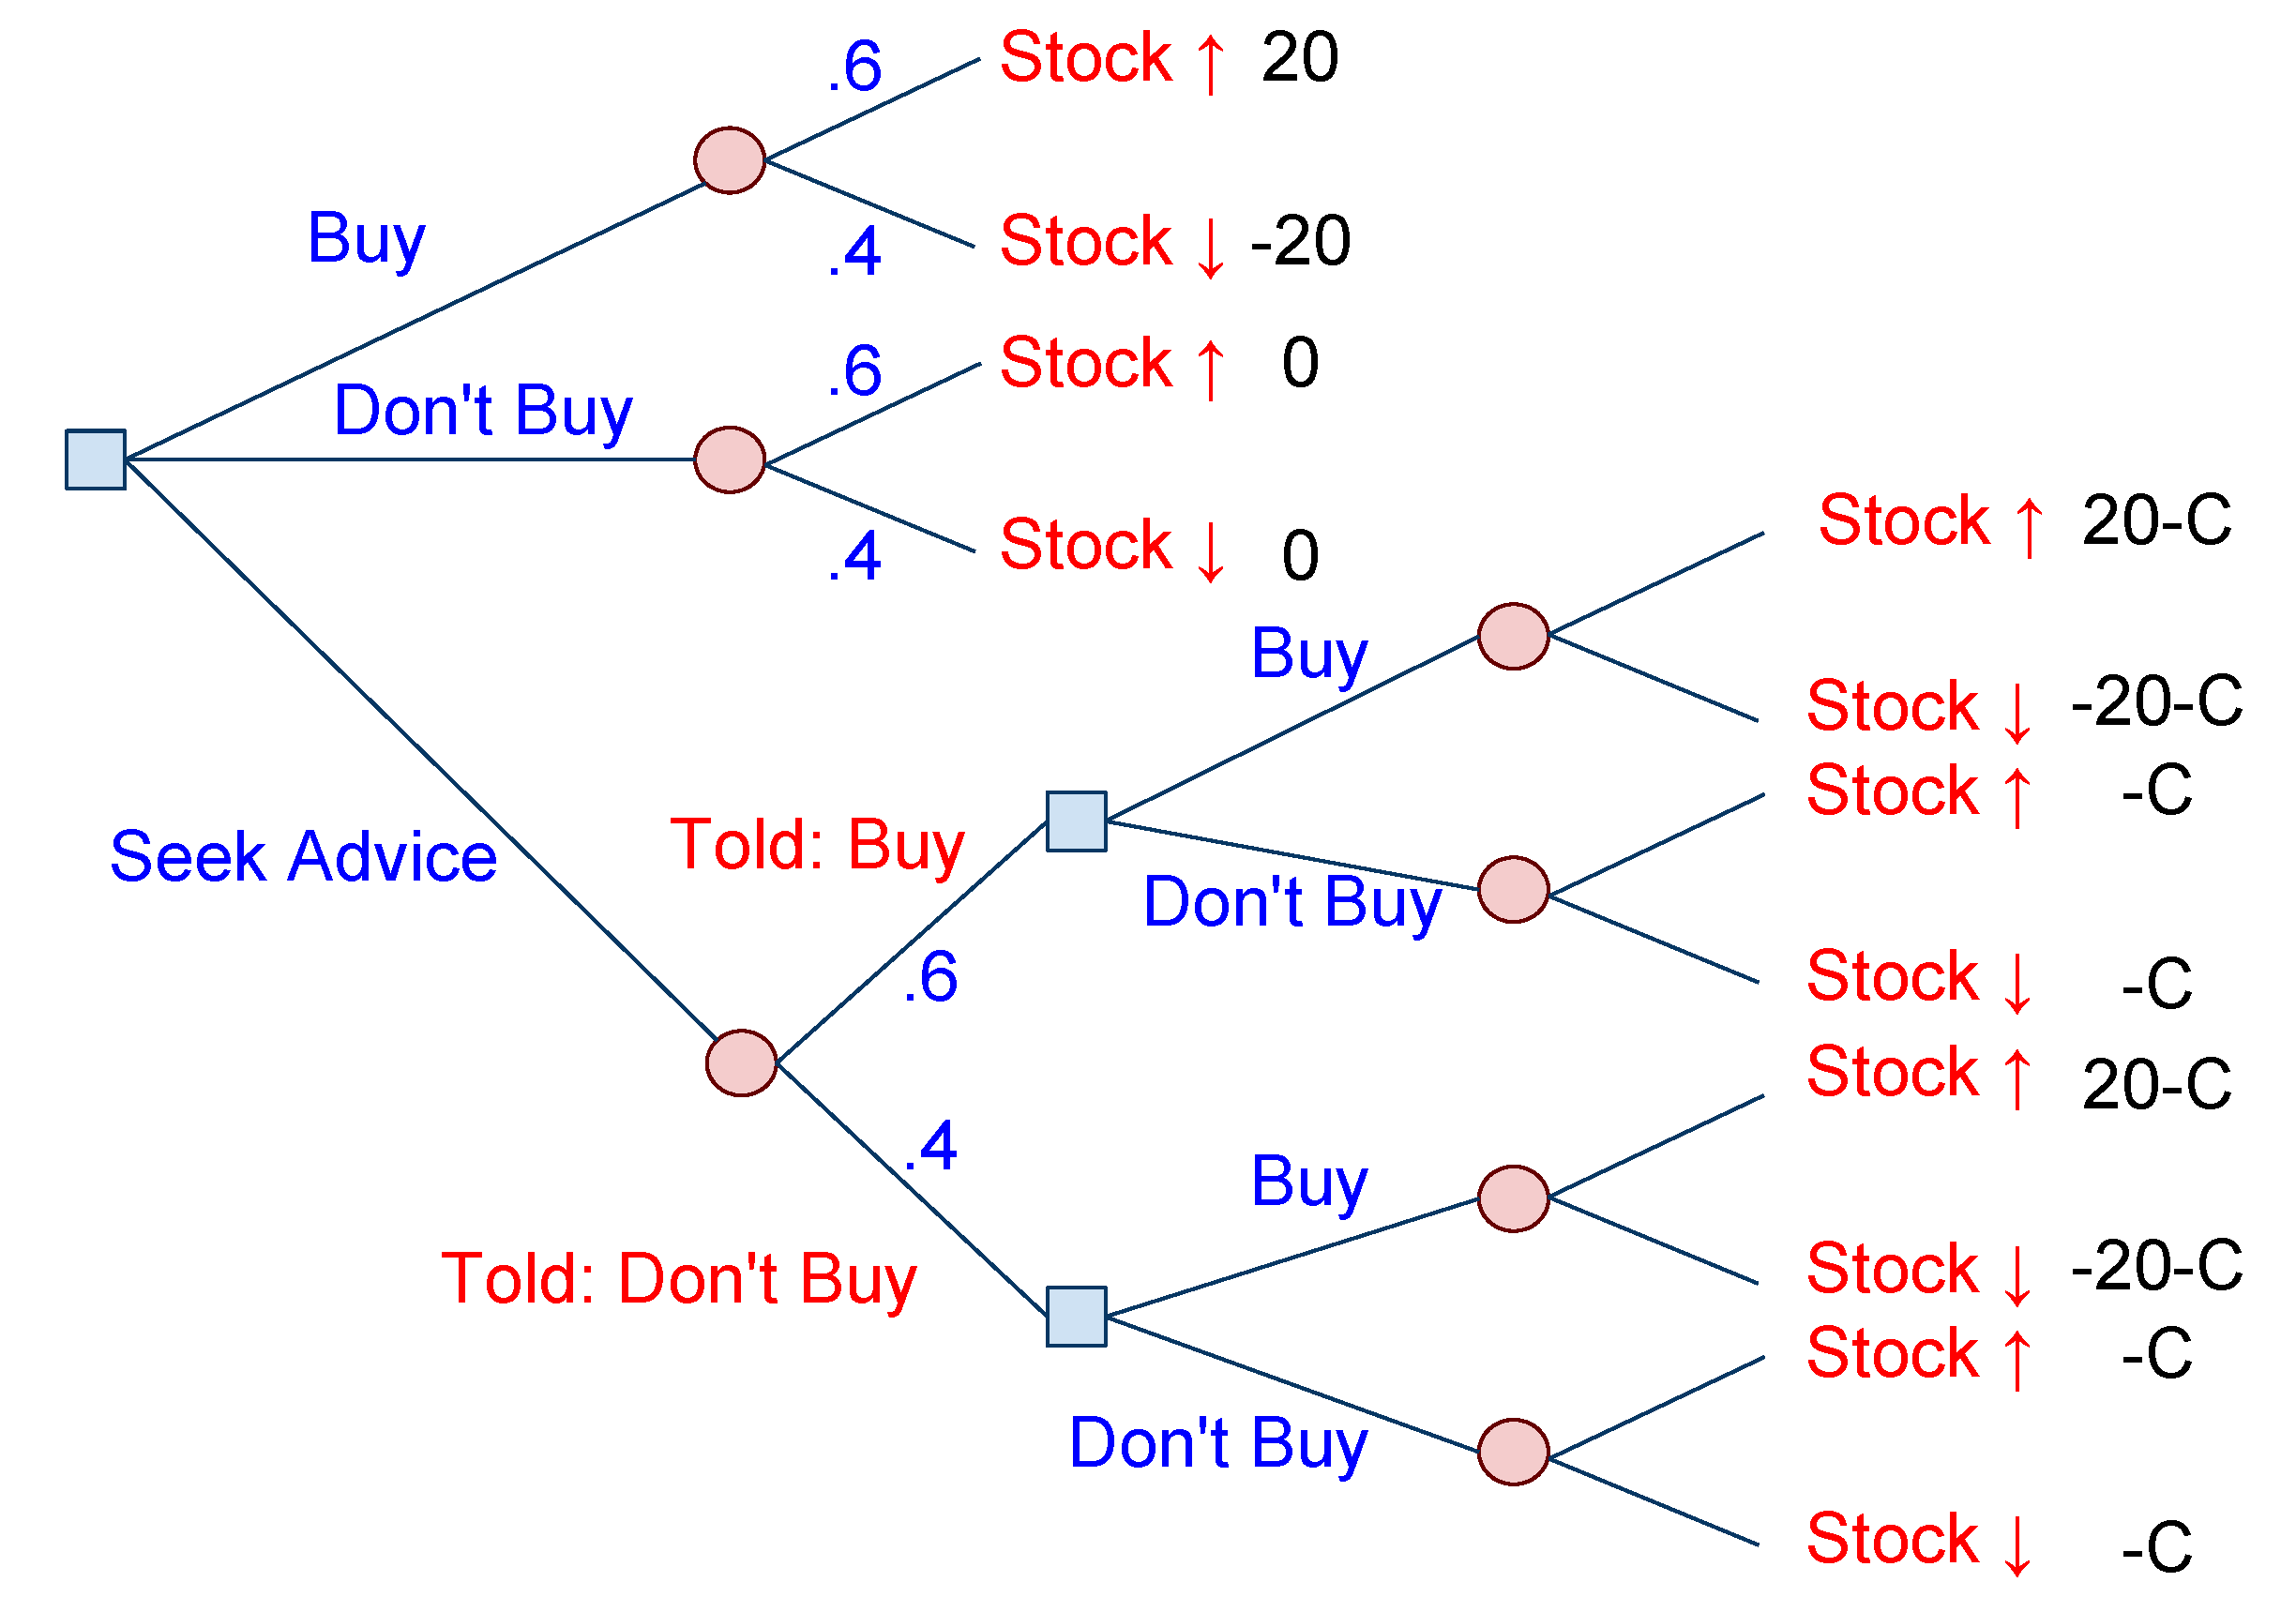
\includegraphics[width=10cm]{Stock_Example_Decision_Tree_7.pdf}
\end{center}}
\only<3>{\begin{center}
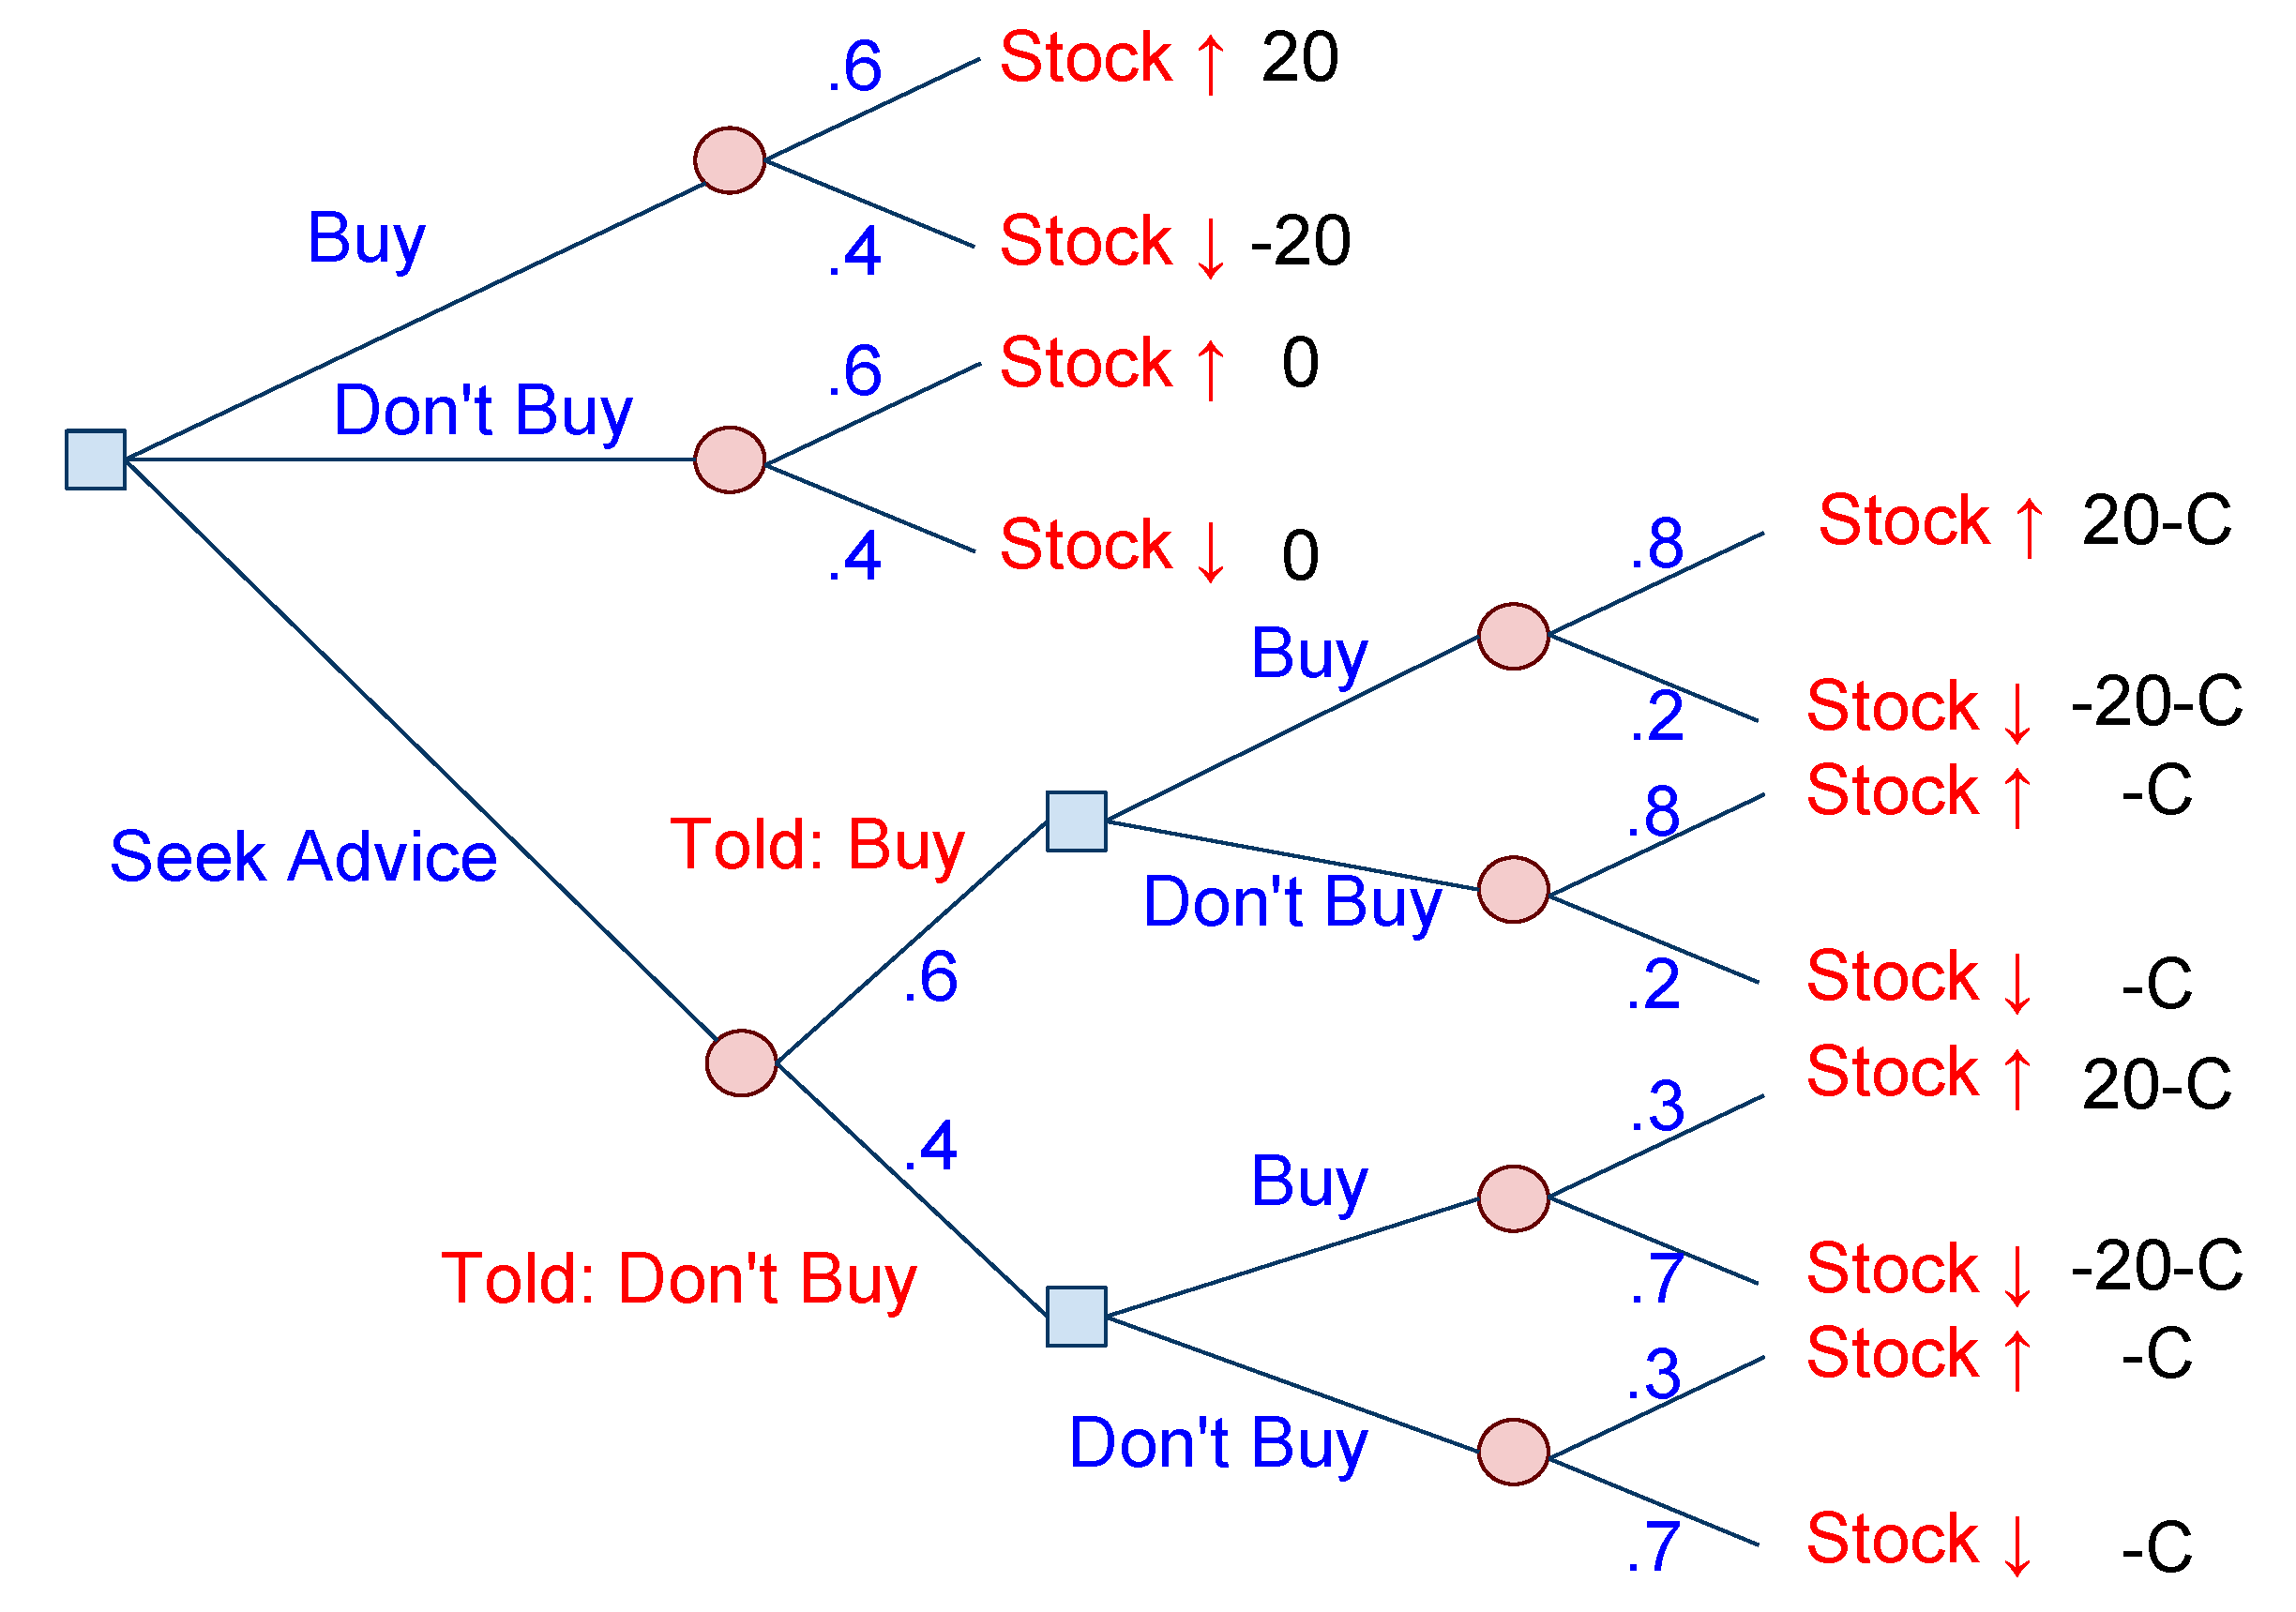
\includegraphics[width=10cm]{Stock_Example_Decision_Tree_8.pdf}
\end{center}}
}


\frame{\frametitle{Step 4: Expected Returns}
Using the conditional probabilities we can calculate the expected return at each options node (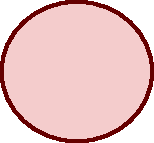
\includegraphics[width=.5cm]{Dot}), working from right to left.\\\vspace{.5cm}
By choosing the decisions that maximise the expected return, we can also work out the expected return at each decision node (
\includegraphics[width=.5cm]{Square}).
}


\frame{\frametitle{Step 4: Expected Returns}
\only<1>{\begin{center}
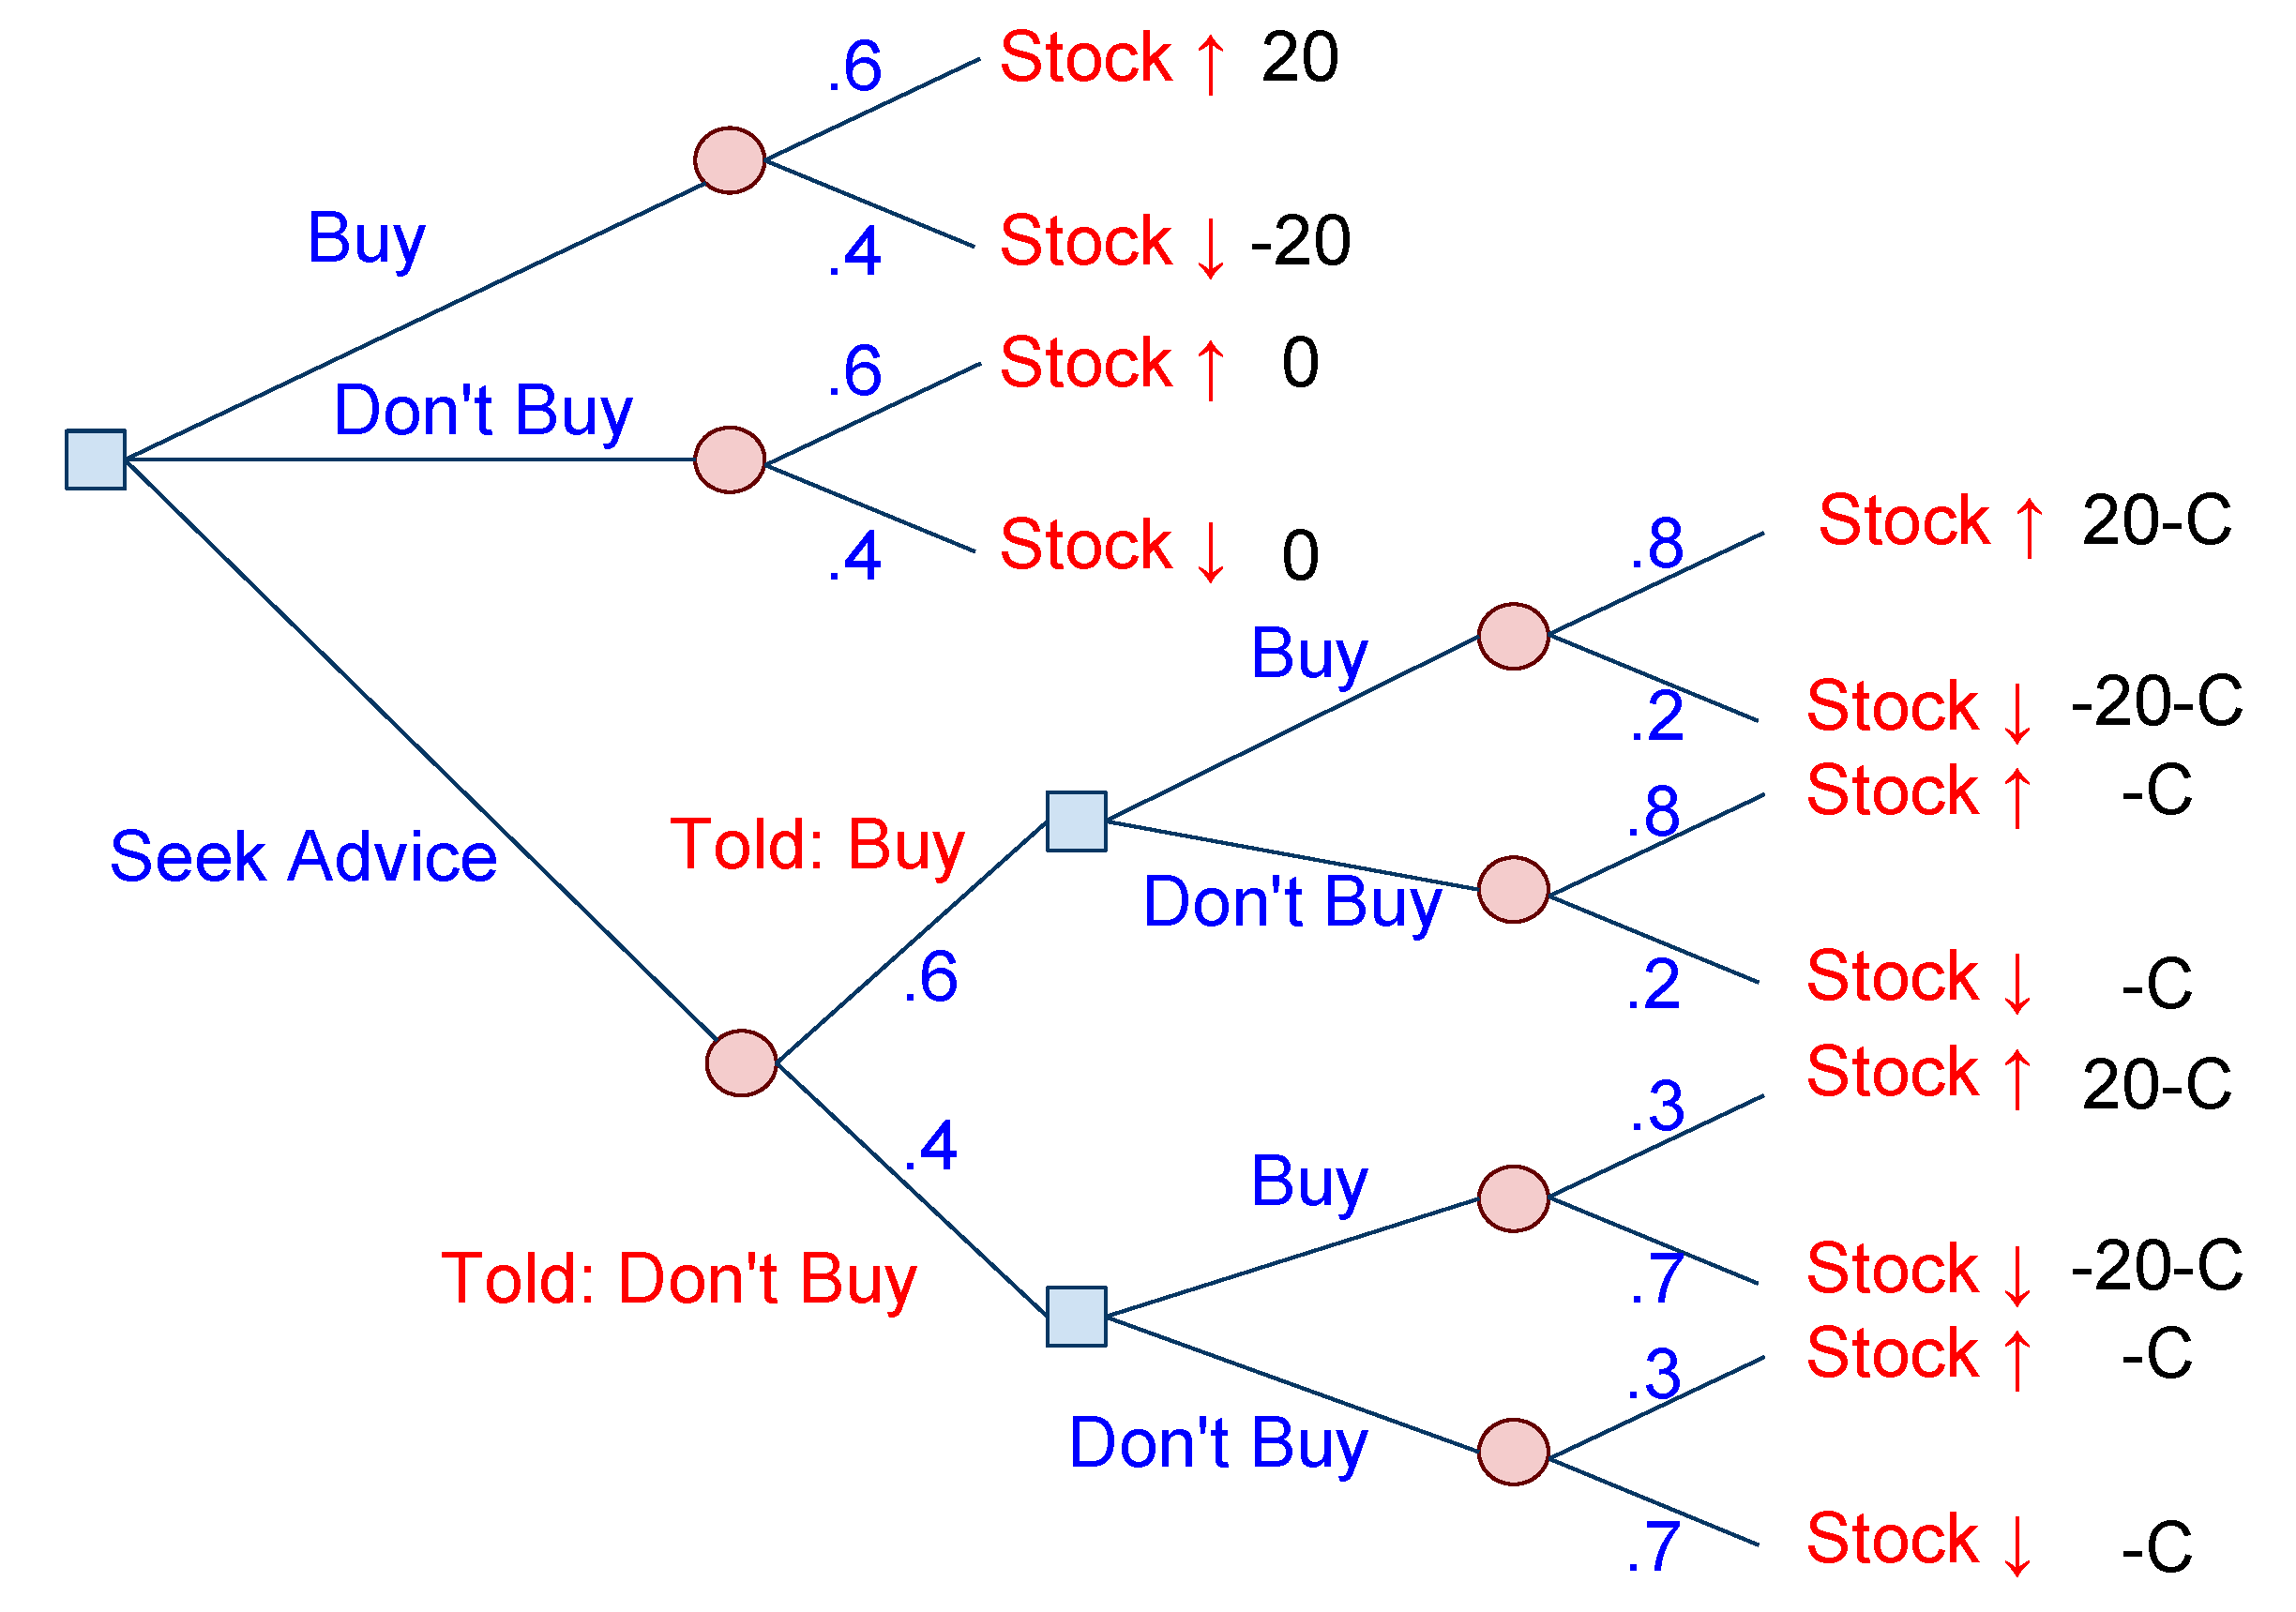
\includegraphics[width=10cm]{Stock_Example_Decision_Tree_8.pdf}
\end{center}}

\only<2>{\begin{center}
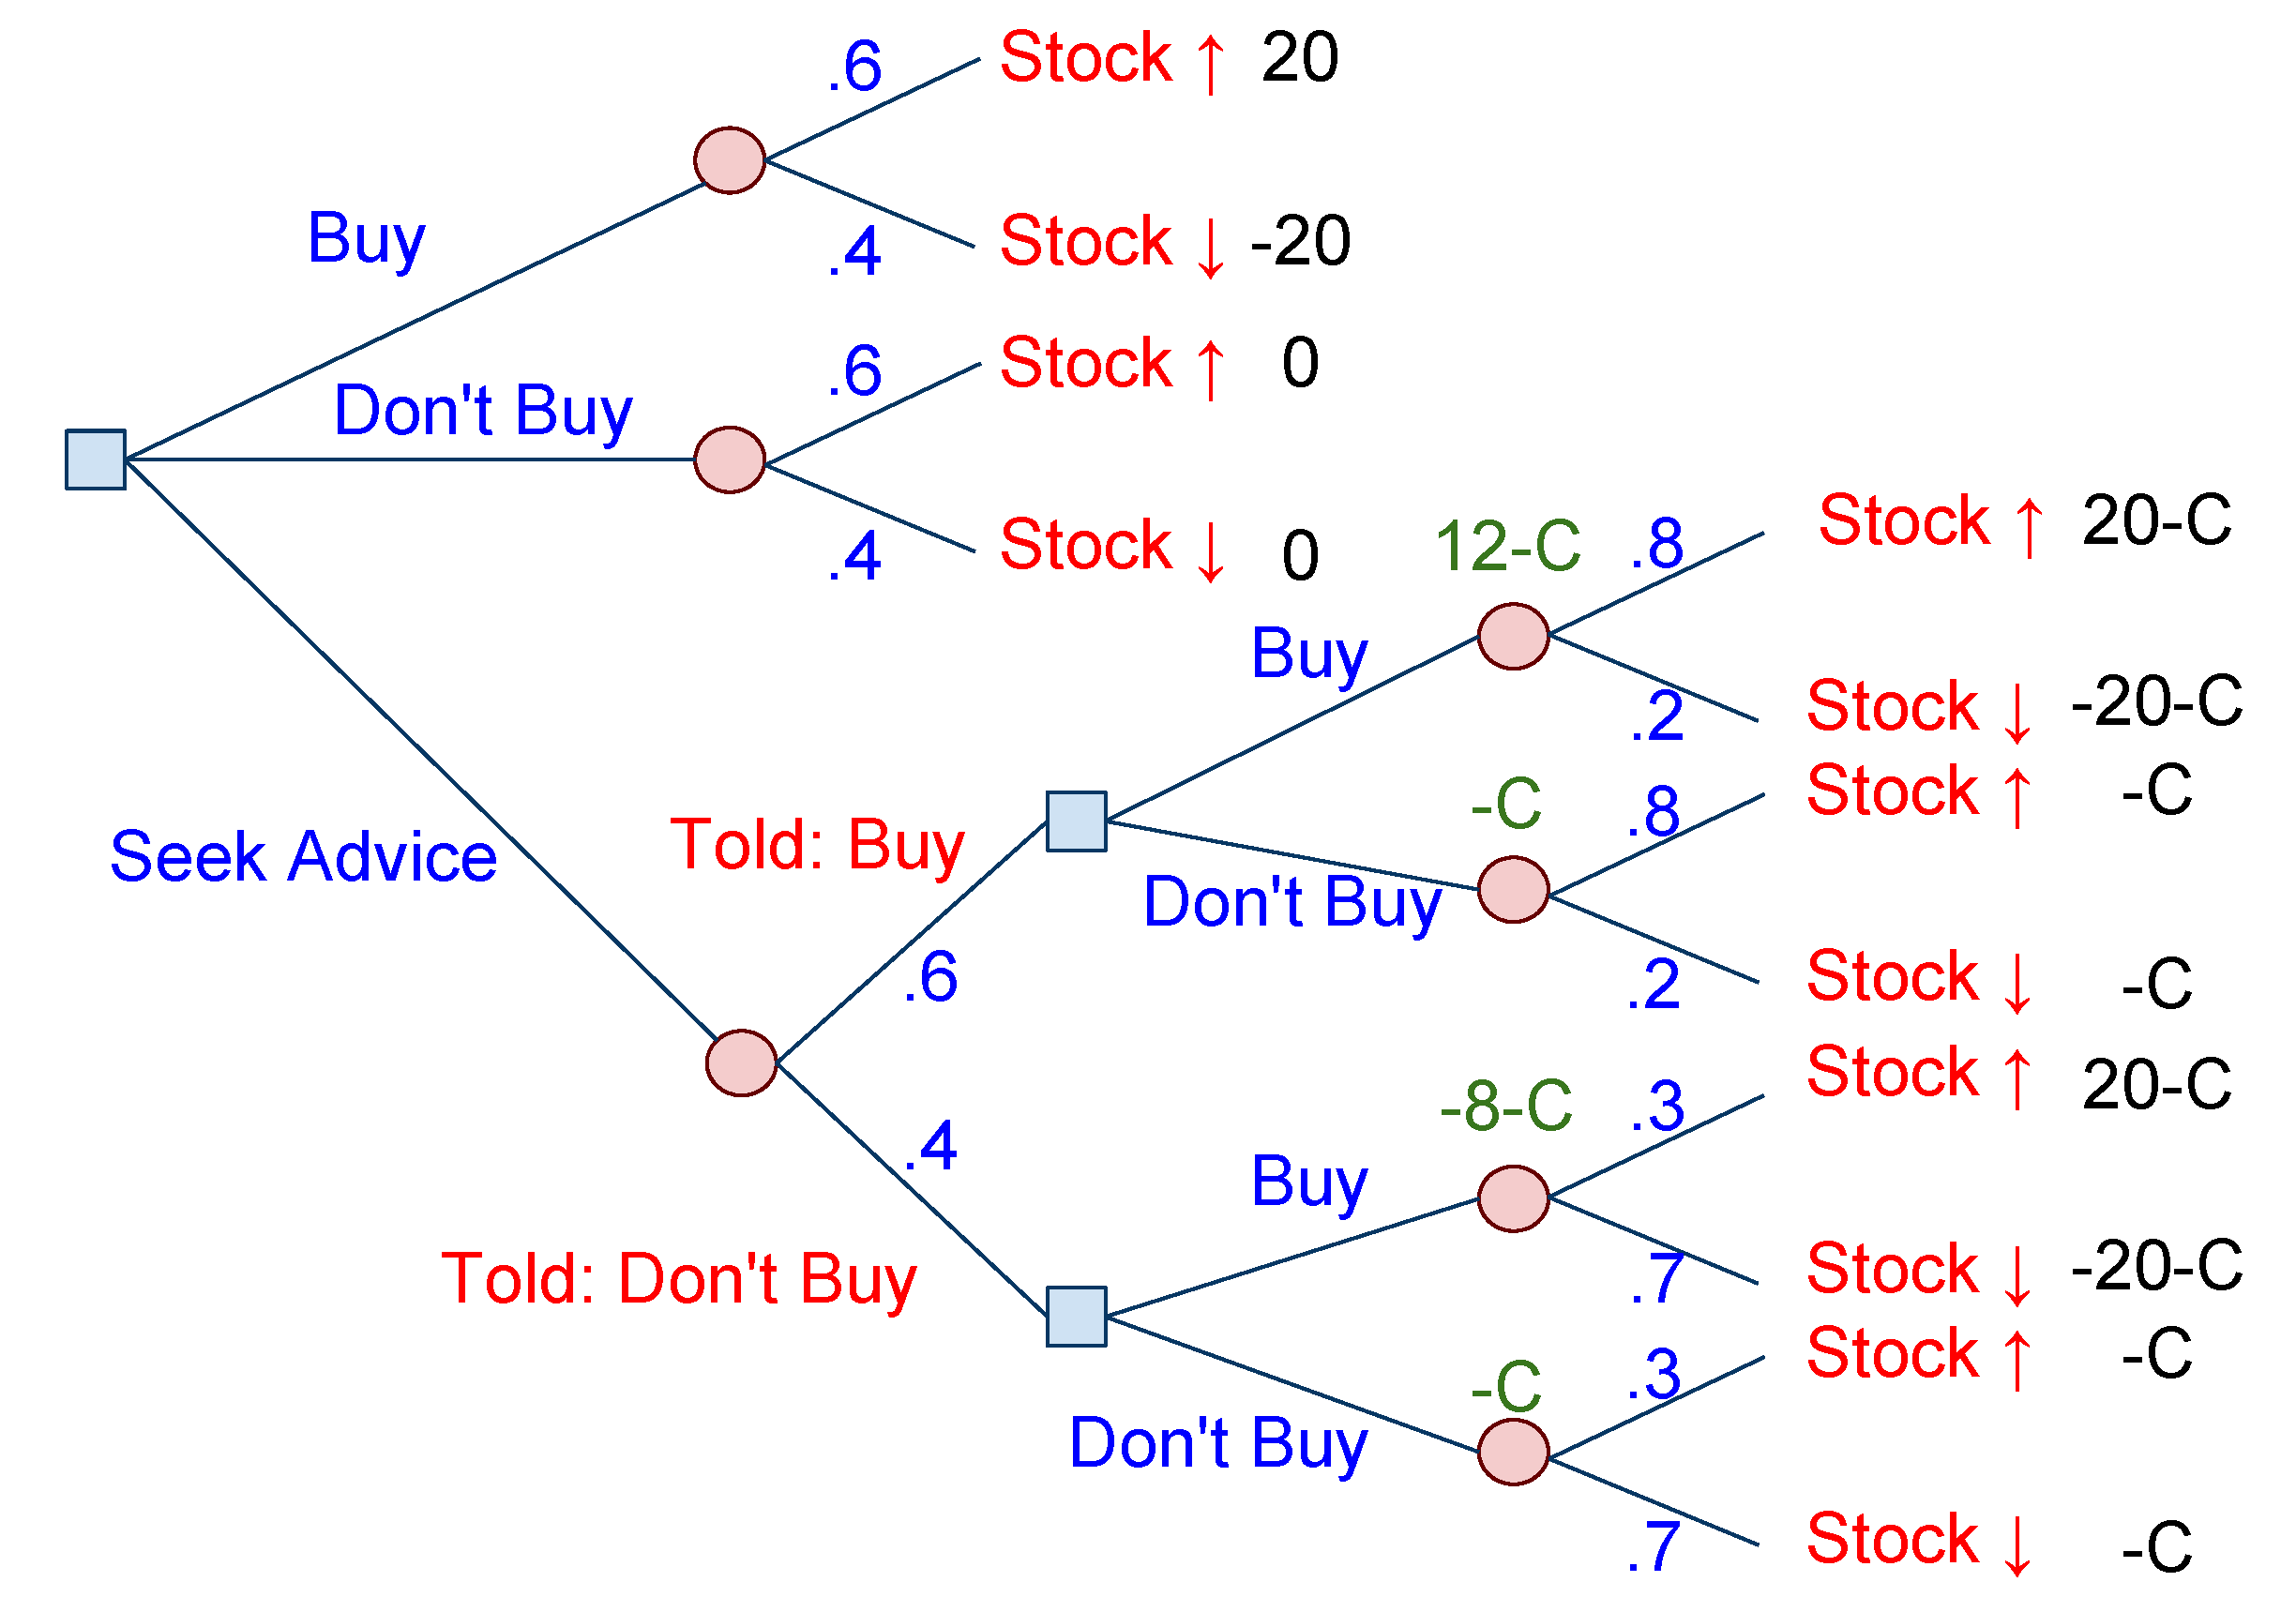
\includegraphics[width=10cm]{Stock_Example_Decision_Tree_9.pdf}
\end{center}}
\only<3>{\begin{center}
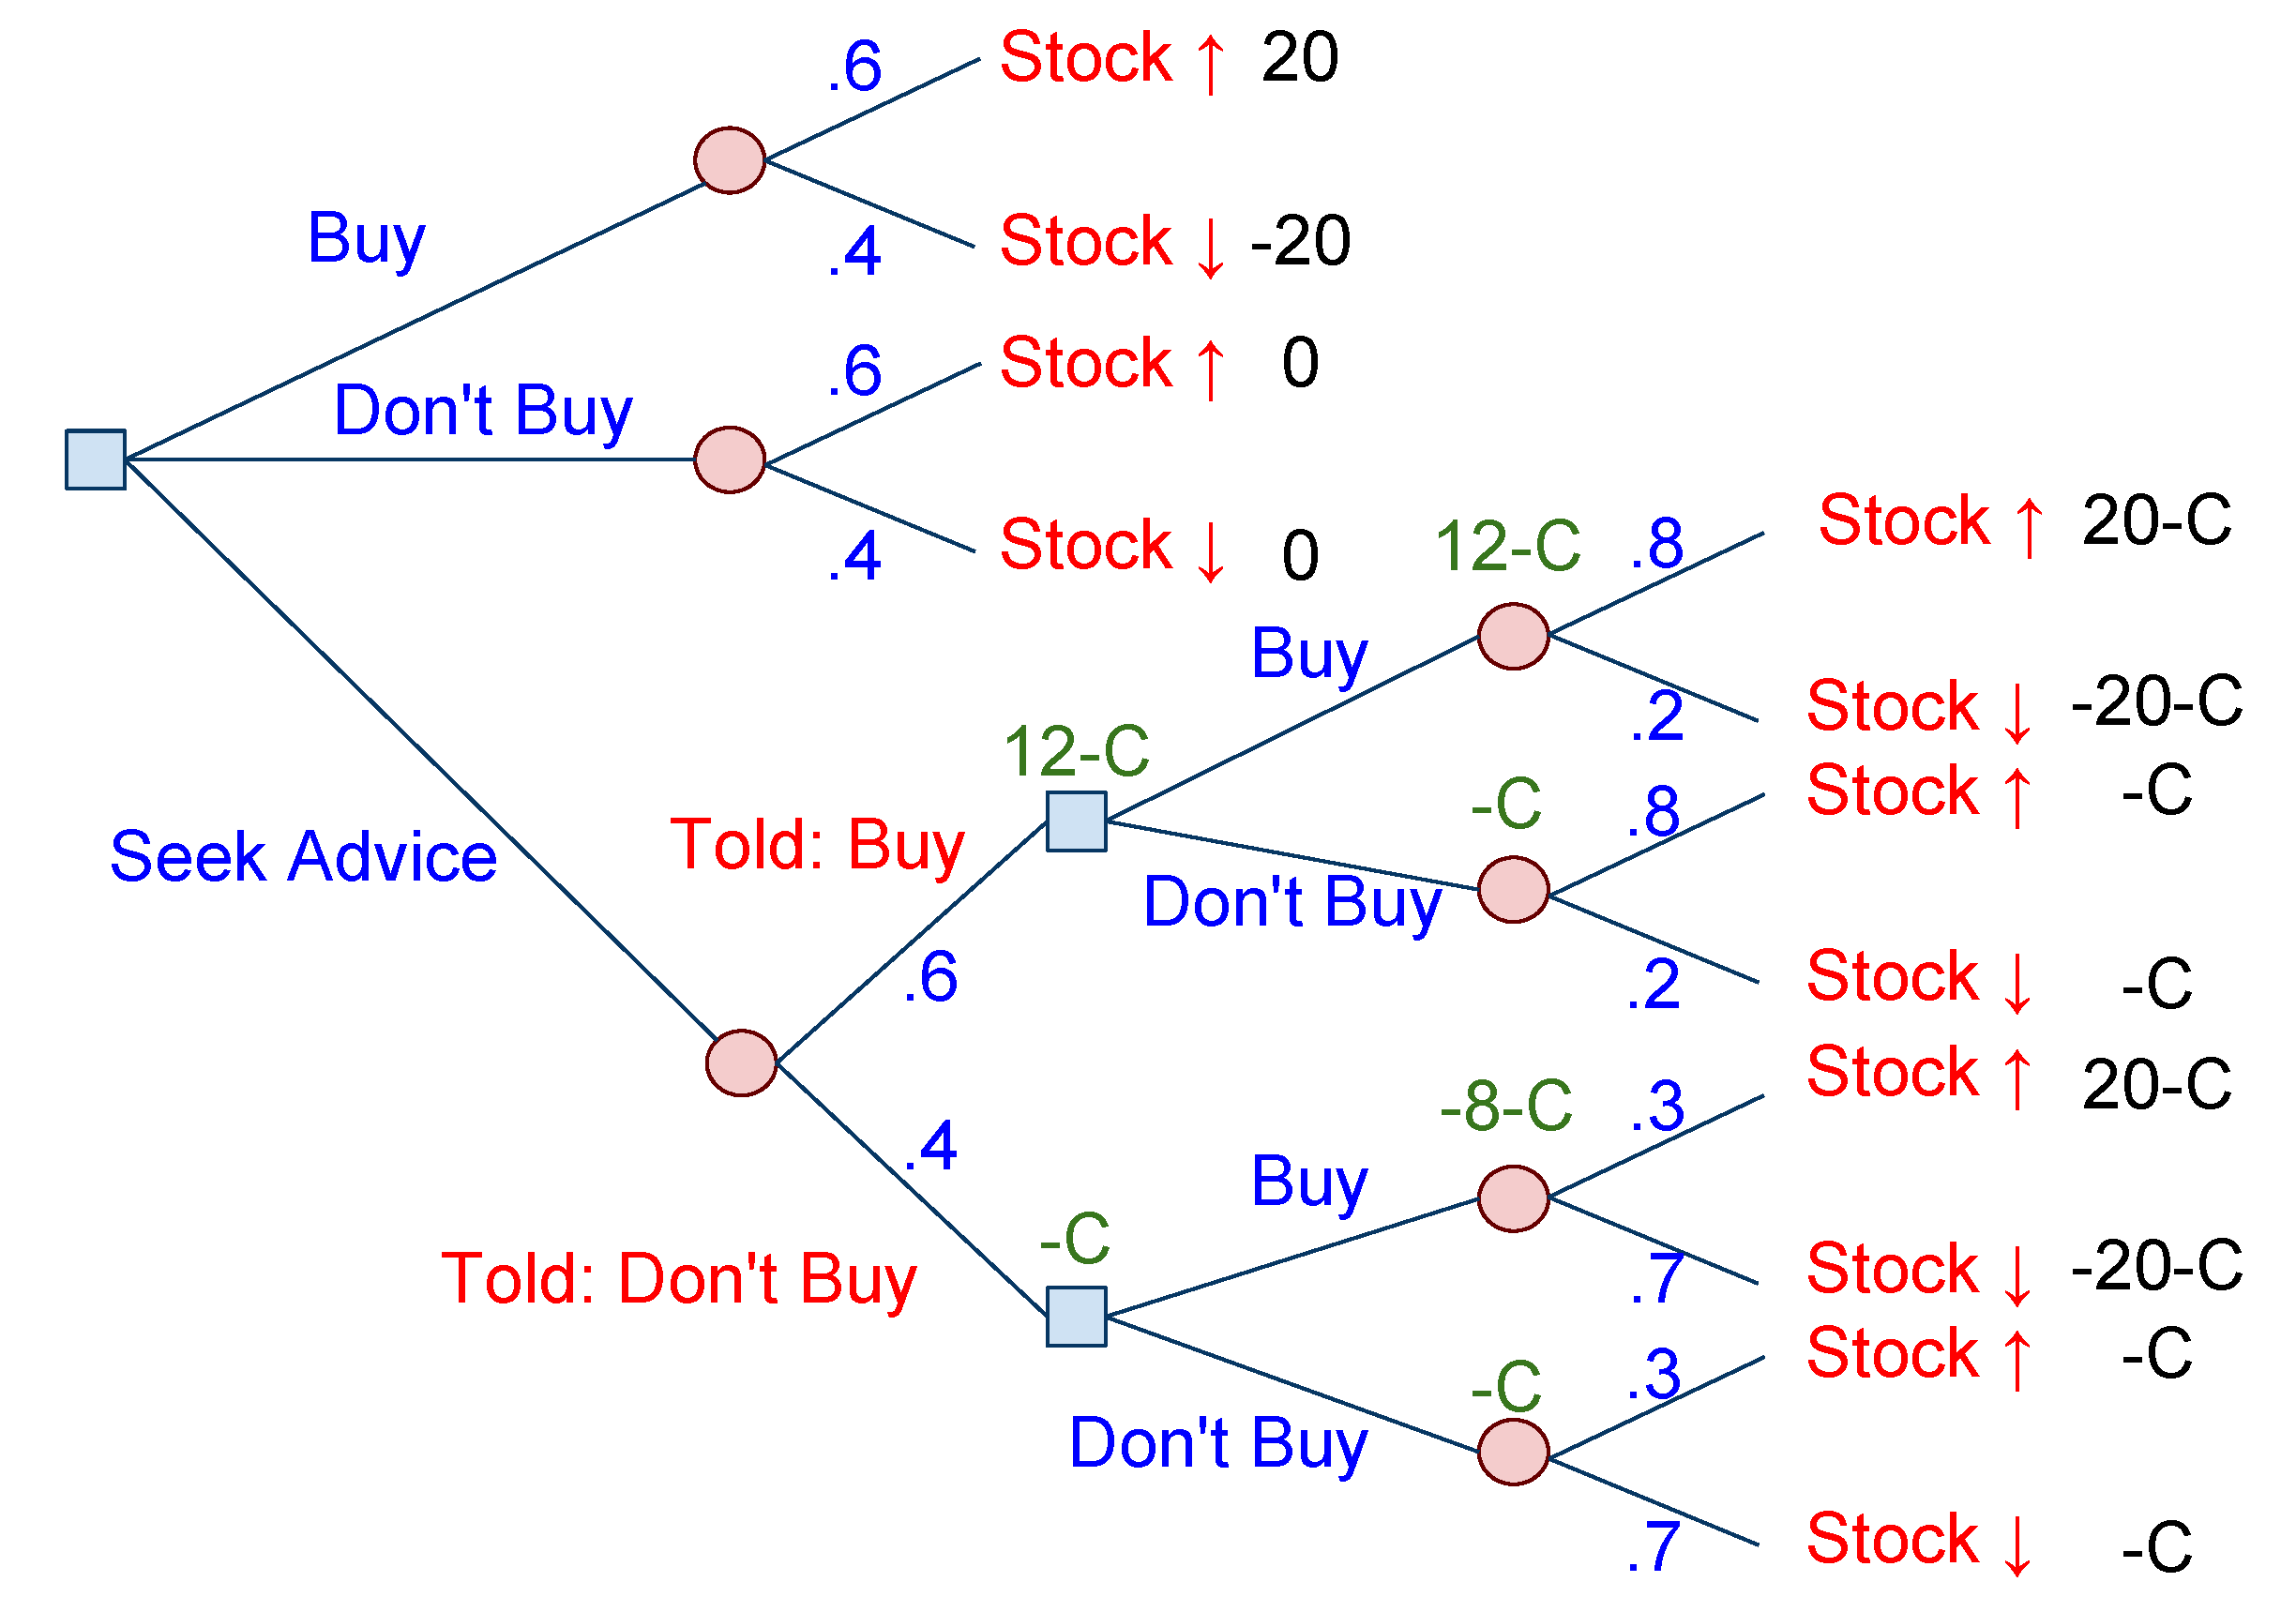
\includegraphics[width=10cm]{Stock_Example_Decision_Tree_10.pdf}
\end{center}}
\only<4>{\begin{center}
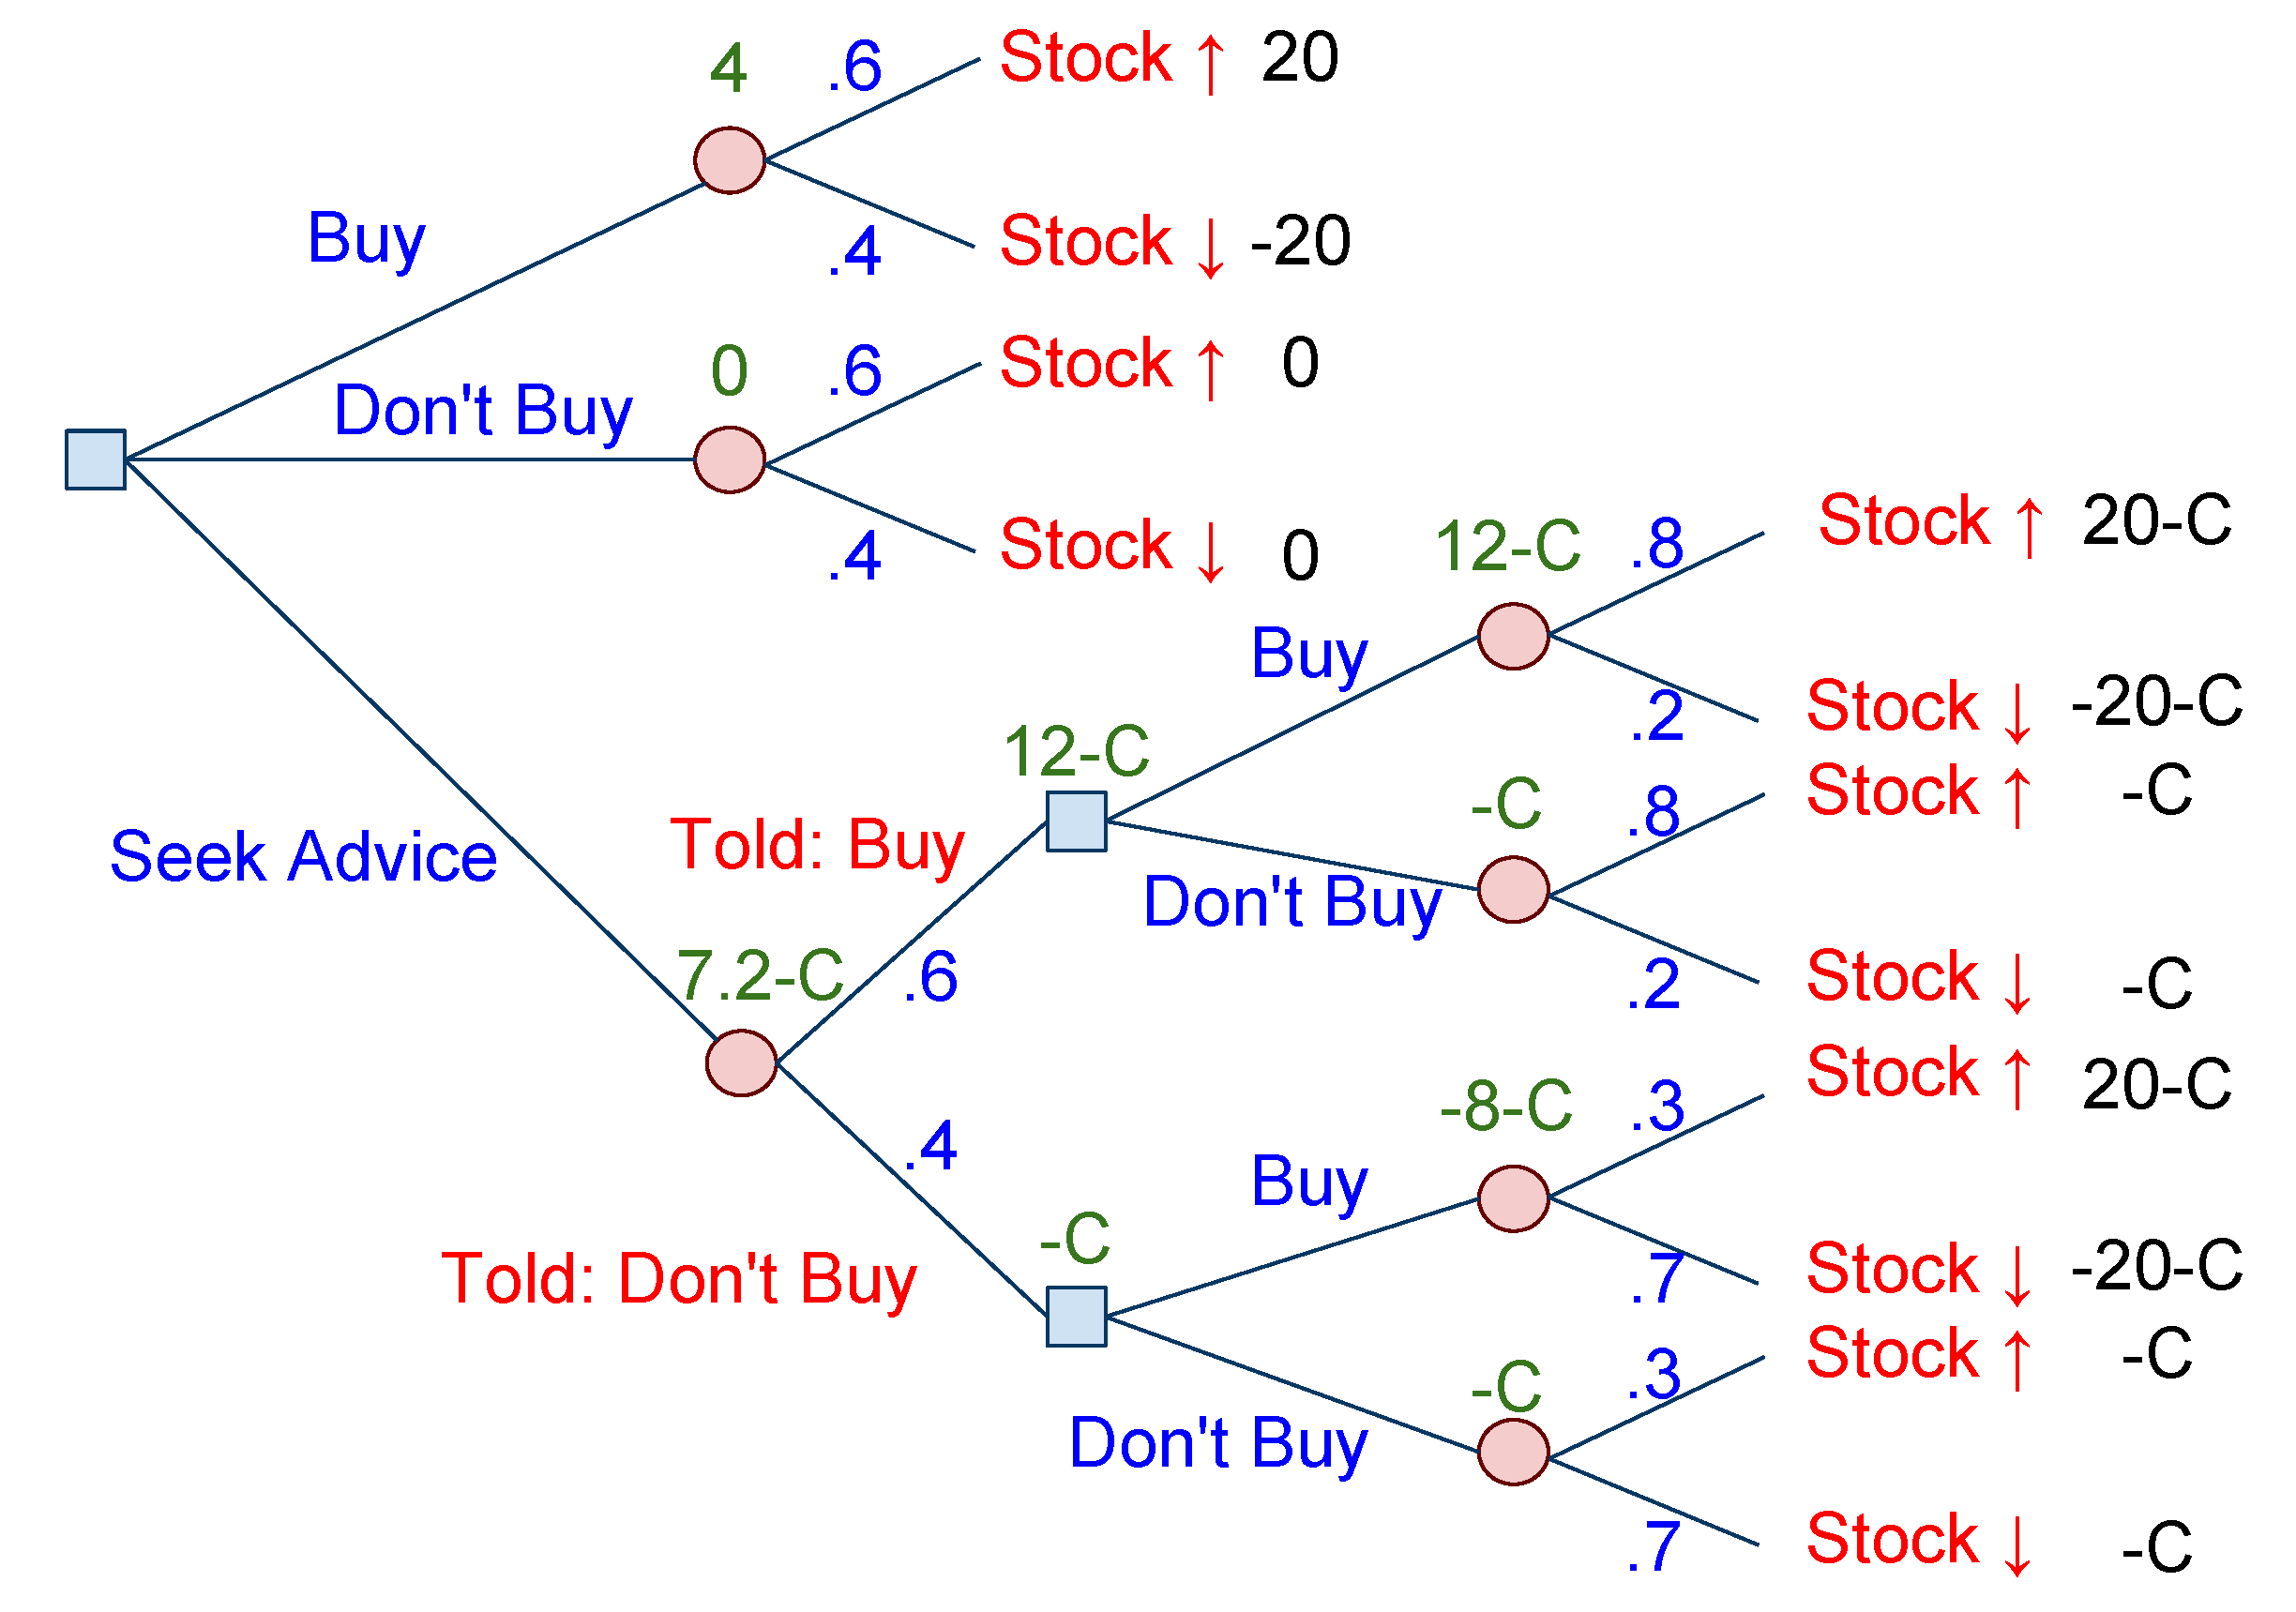
\includegraphics[width=10cm]{Stock_Example_Decision_Tree_11.pdf}
\end{center}}
}

\frame{\frametitle{Example}
Consider the following example:
\begin{itemize}
\item Decide to not toss a coin and receive 4.
\item Toss an unbiased coin :
\begin{itemize}
\item heads: receive 10.
\item tails: receive nothing.
\end{itemize}
\end{itemize}}

\frame{\frametitle{Example}
\only<1>{\begin{center}
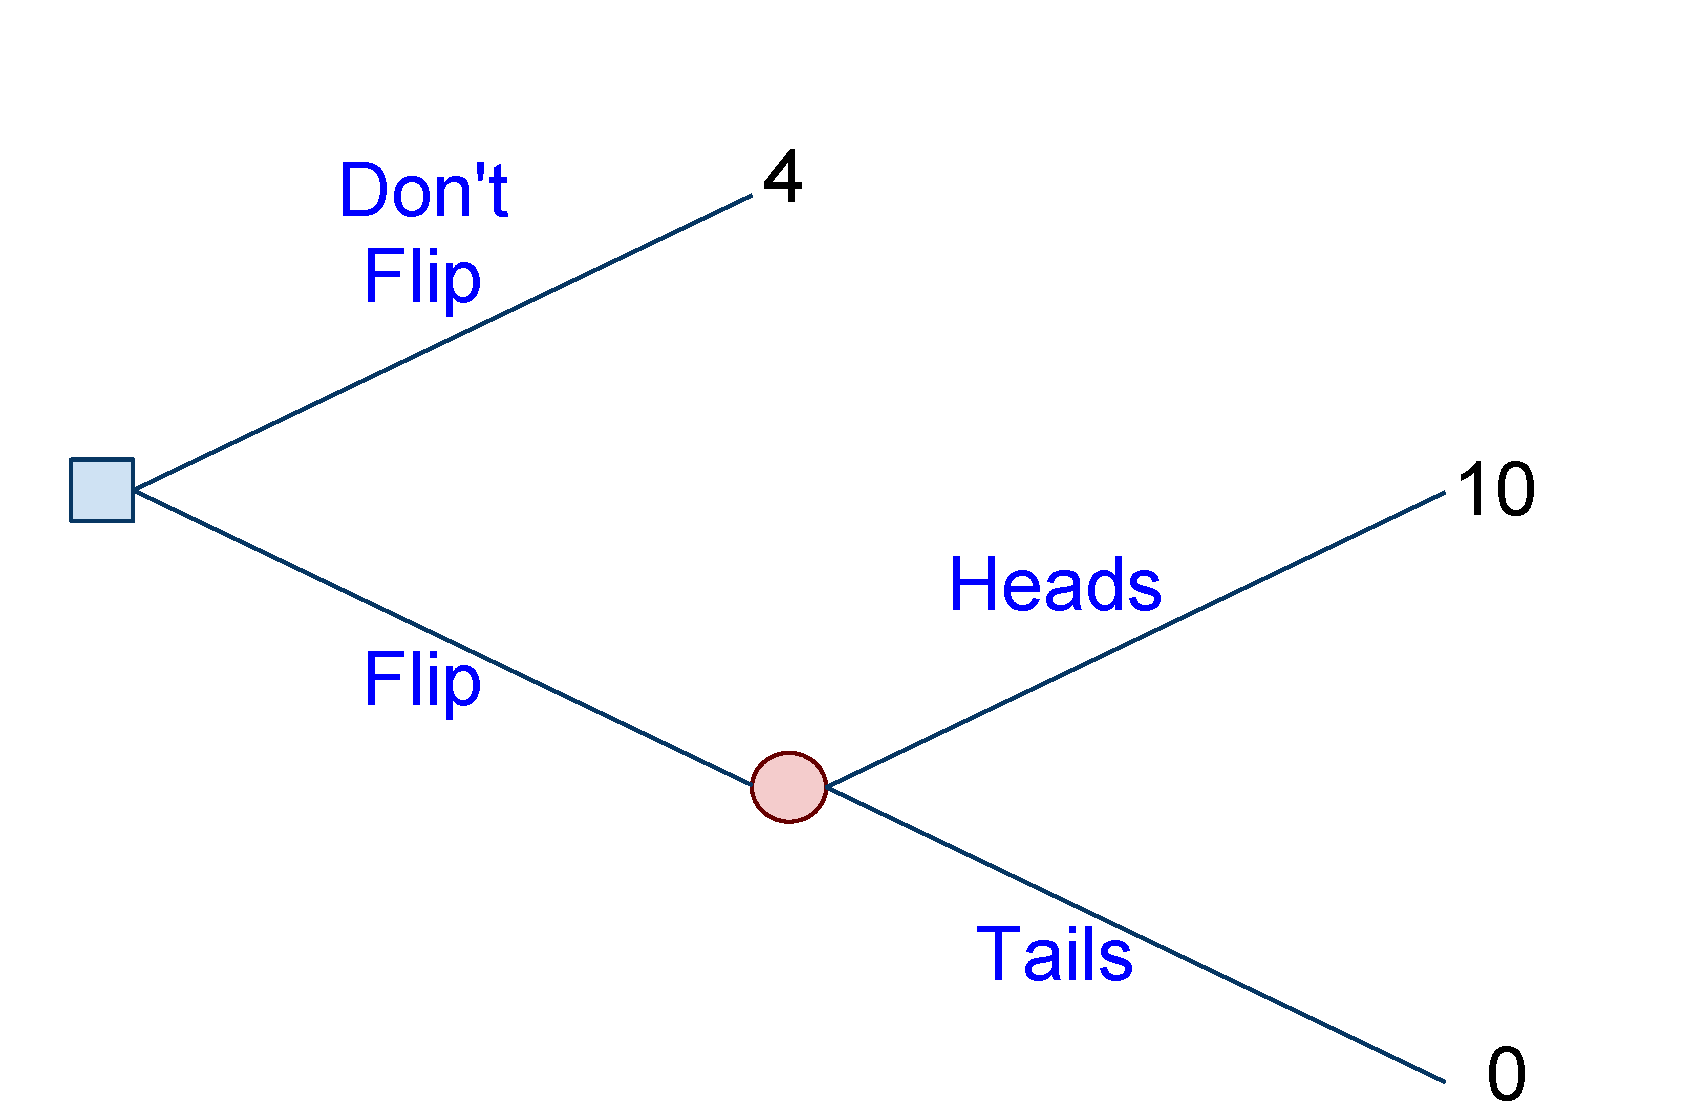
\includegraphics[width=7cm]{Coin_Flip_1.pdf}
\end{center}}
\only<2>{\begin{center}
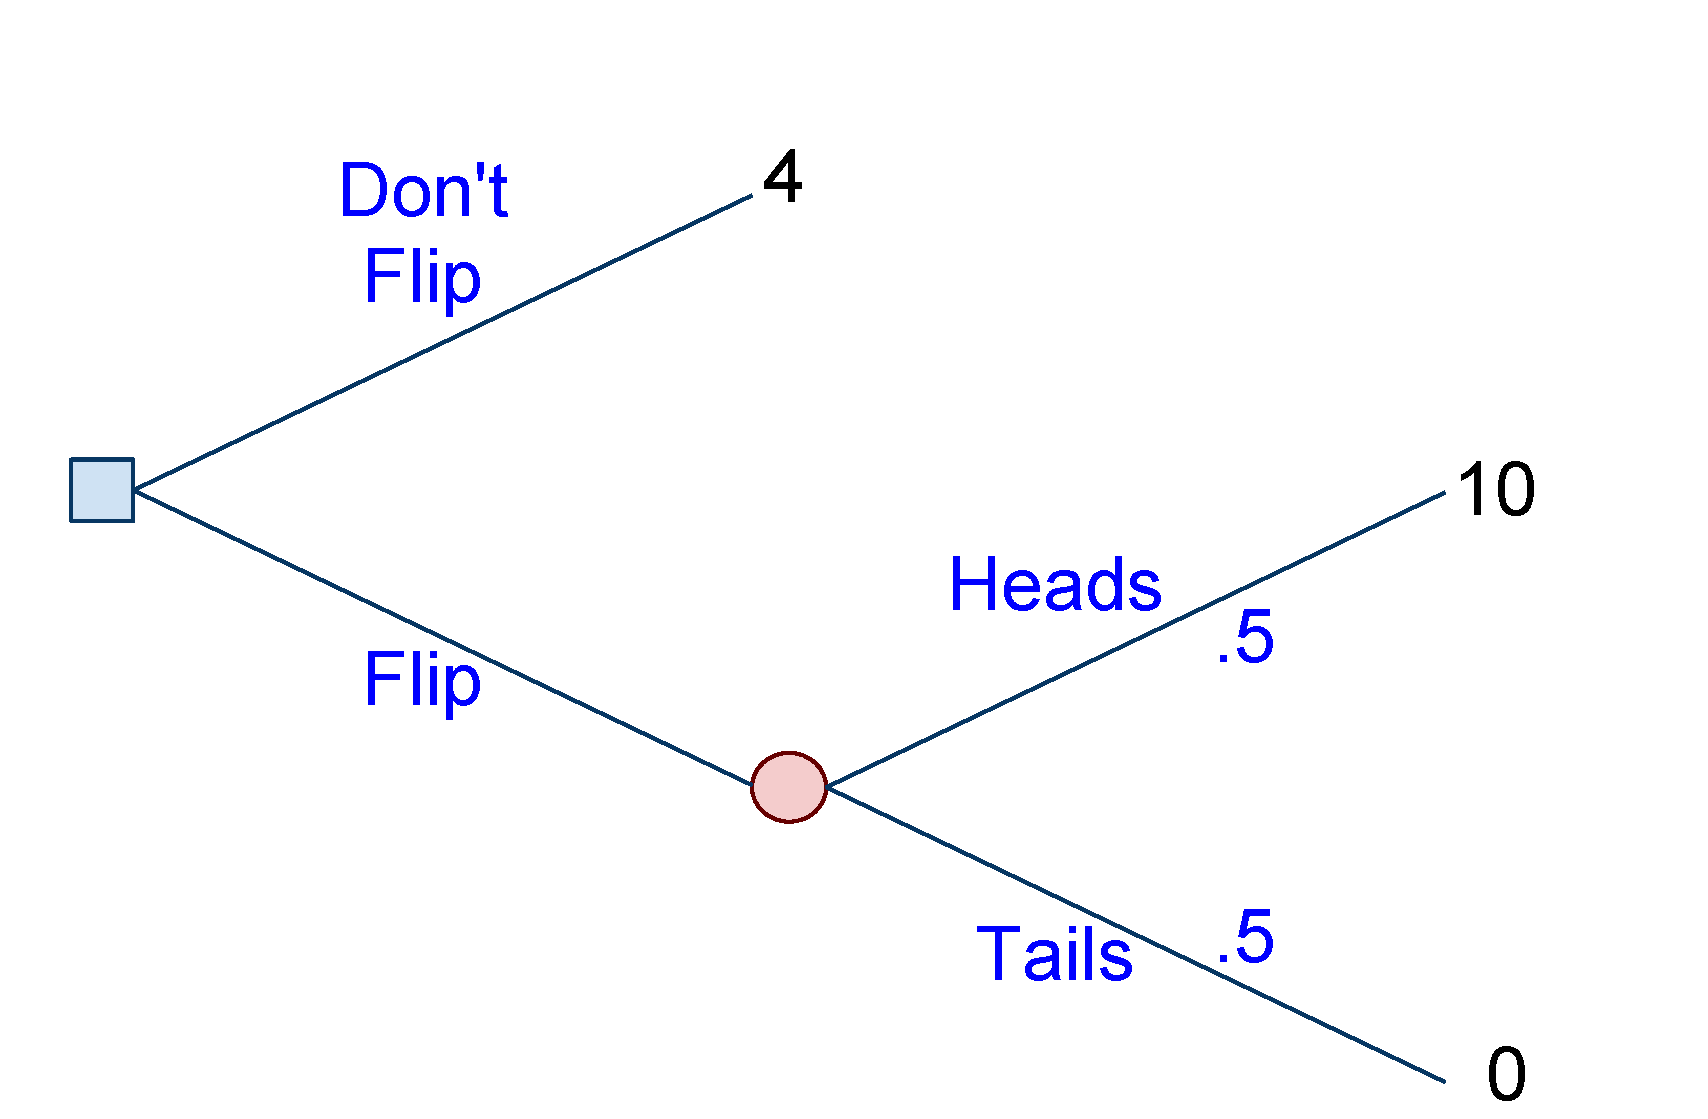
\includegraphics[width=7cm]{Coin_Flip_2.pdf}
\end{center}}
\only<3>{\begin{center}
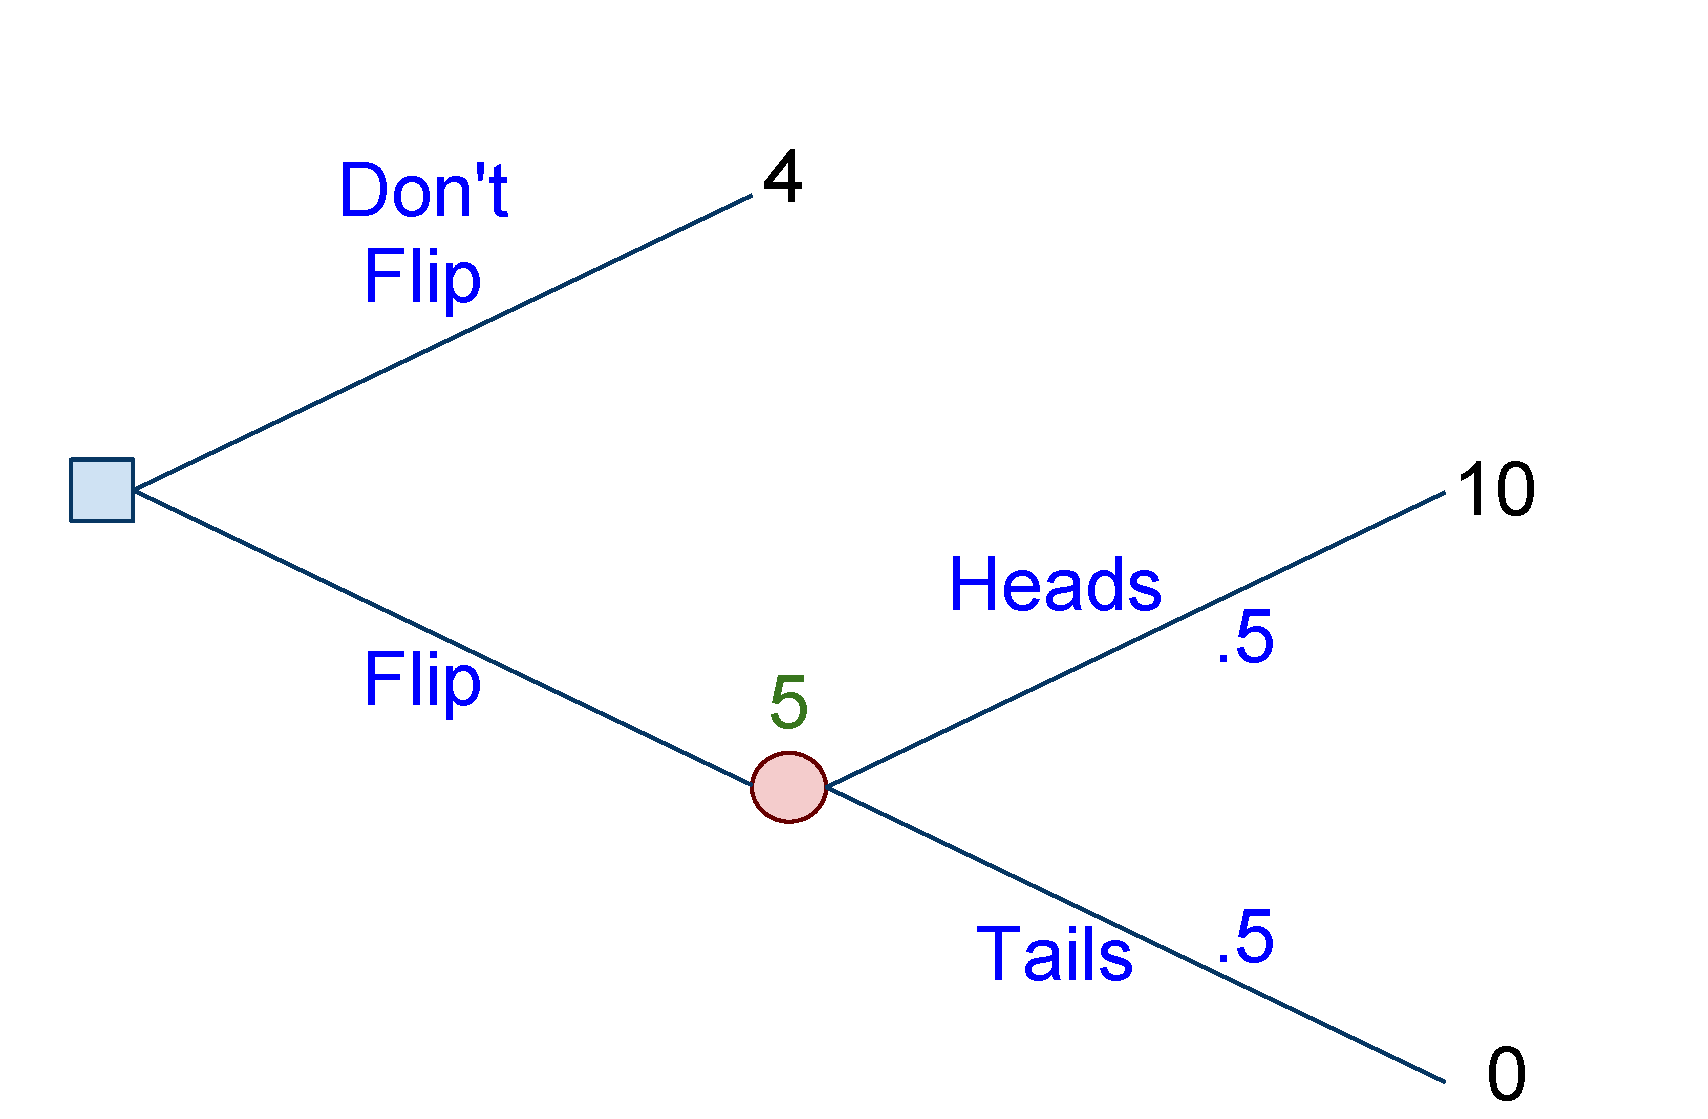
\includegraphics[width=7cm]{Coin_Flip_3.pdf}
\end{center}}
}


\section{Basic Utility Functions}
\frame{\frametitle{Utility functions}}
\frame{\frametitle{Utility Functions}
We would like to reflect different opinions about the value of certain gain versus uncertain gain, but still be able to make use of decision trees. We need a way of transforming absolute gain to an appropriate scale that reflects the decision maker's preference. This scale is called a \emph{utility function}.
}

\frame{\frametitle{Example}
For example consider the utility function: $u:\mathbb{R}\to\mathbb{R}$:
$$u(x)=\sqrt{x}$$\pause
\only<1>{\begin{center}
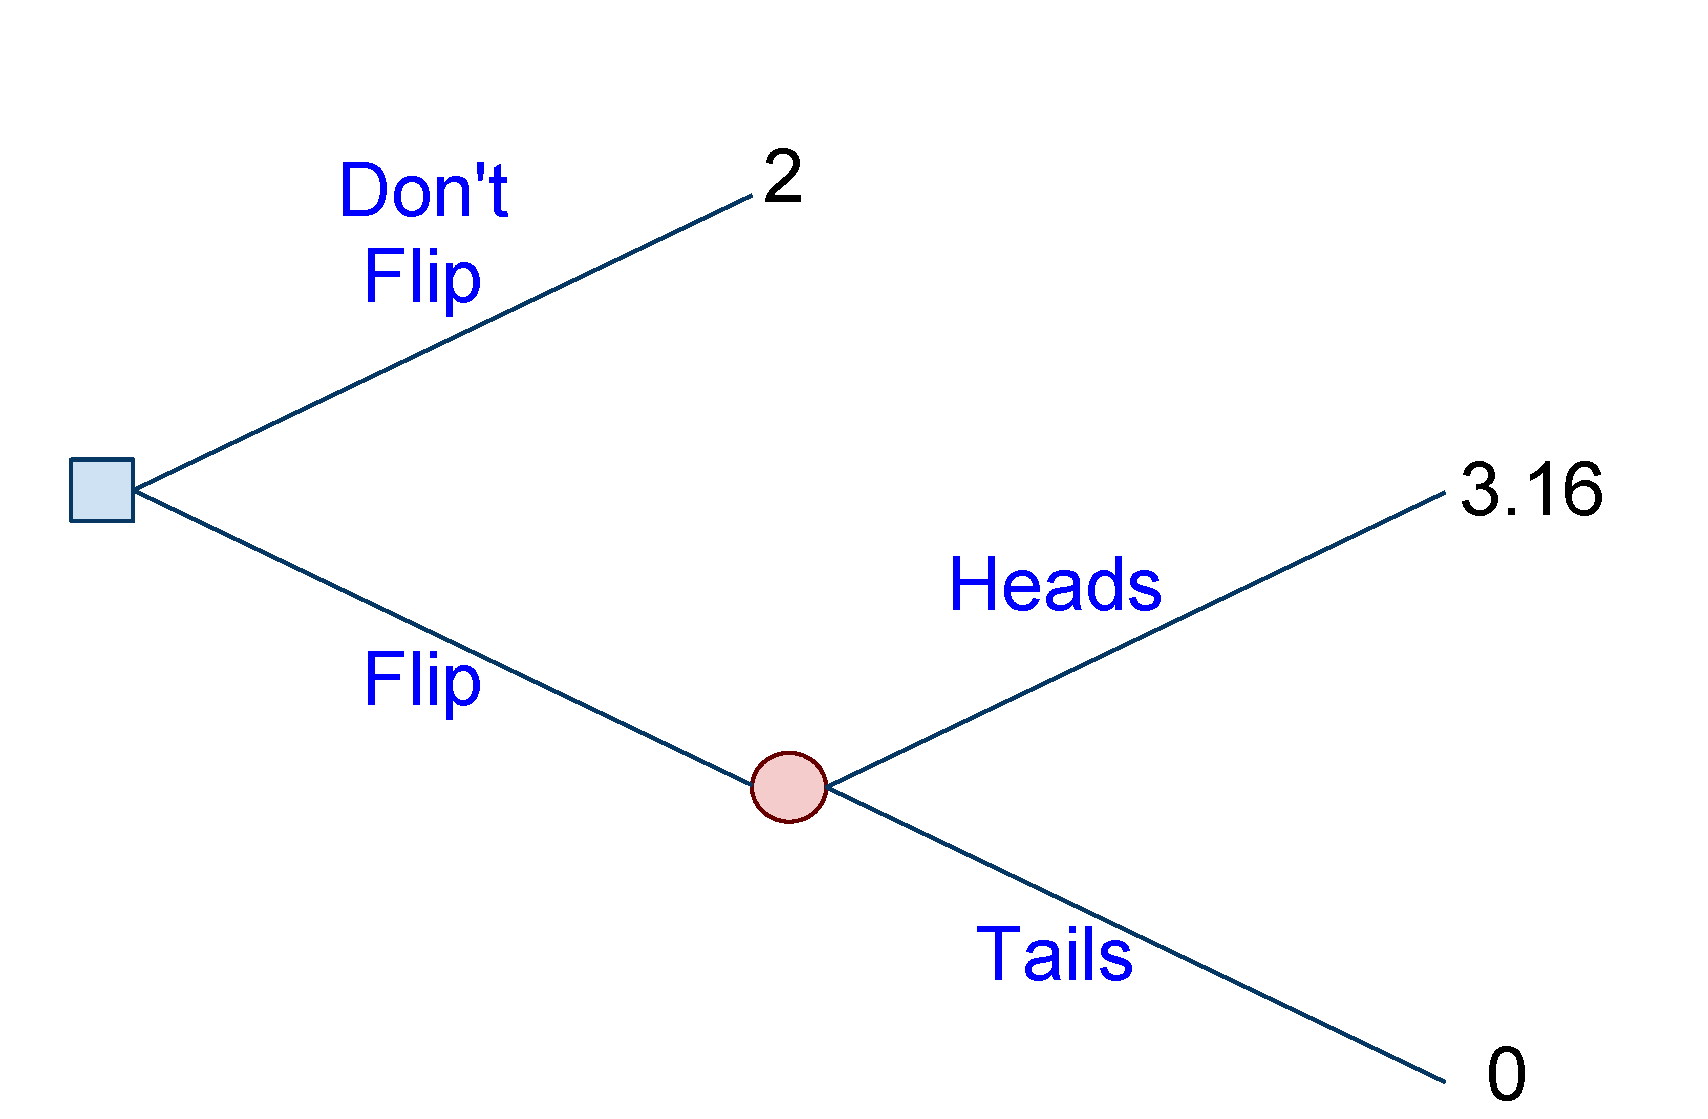
\includegraphics[width=7cm]{Coin_Flip_with_utility_1.pdf}
\end{center}}
\only<2>{\begin{center}
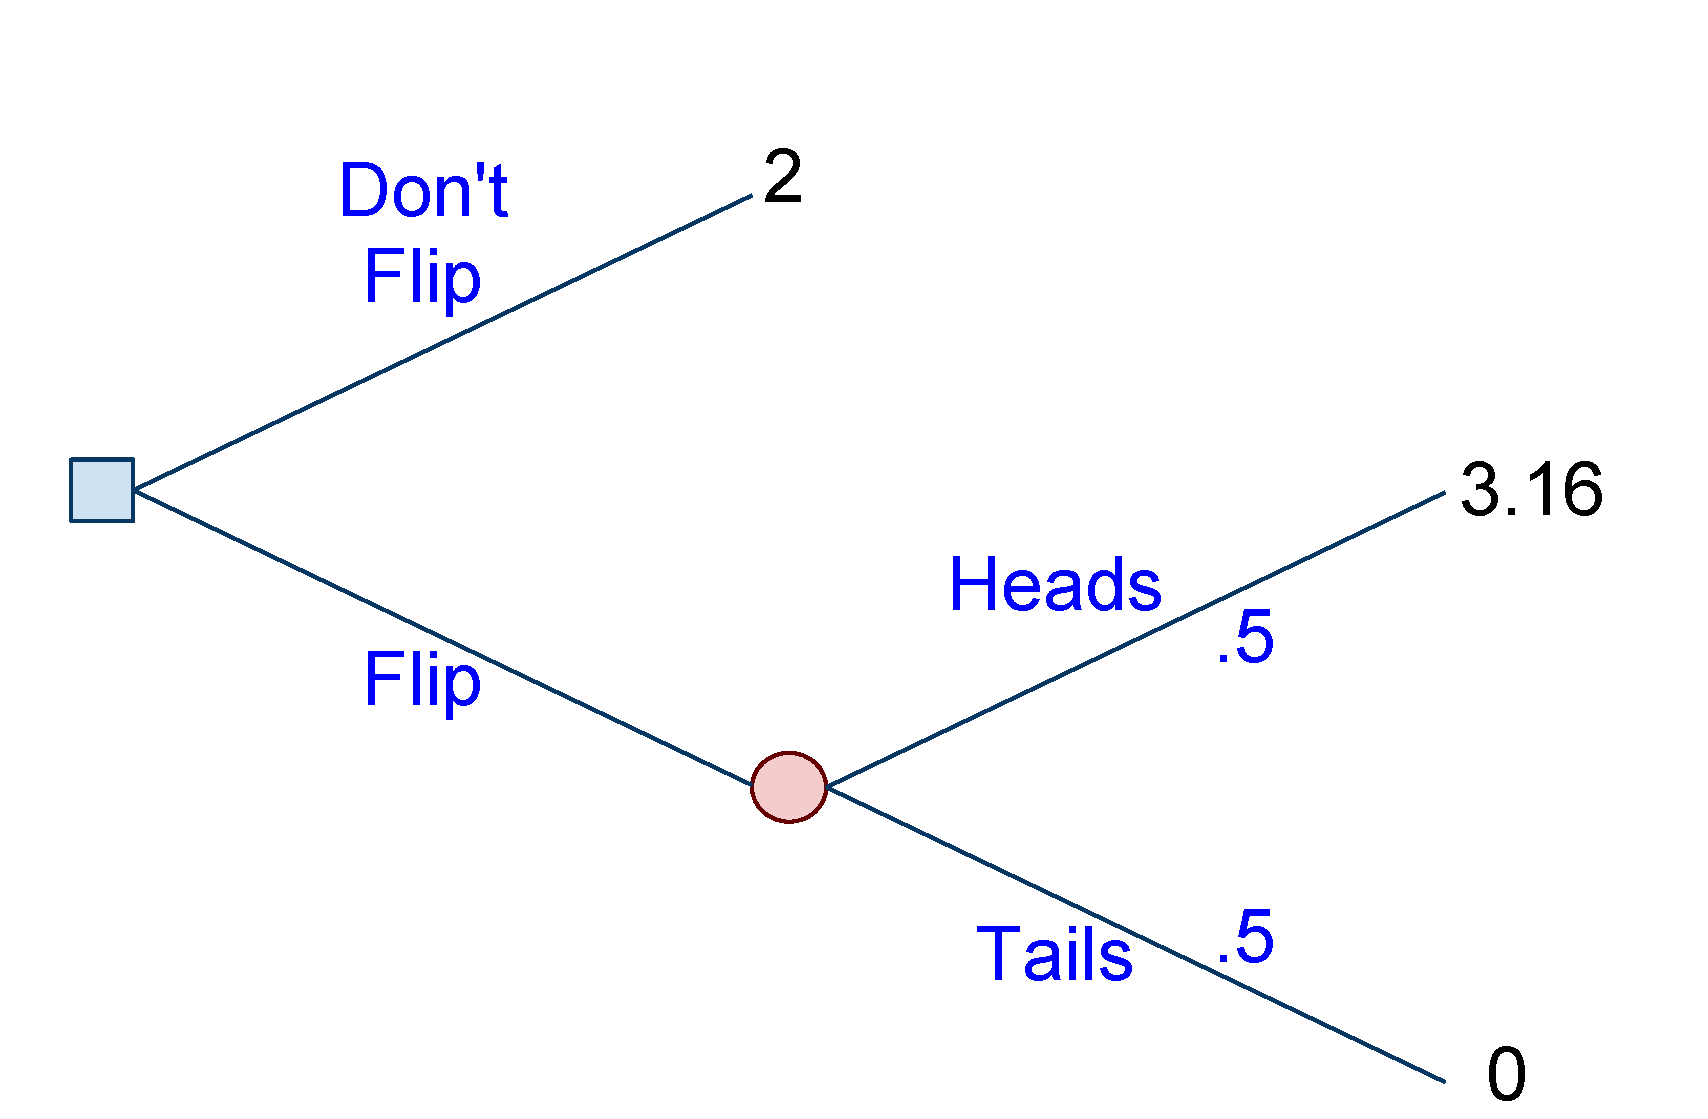
\includegraphics[width=7cm]{Coin_Flip_with_utility_2.pdf}
\end{center}}
\only<3>{\begin{center}
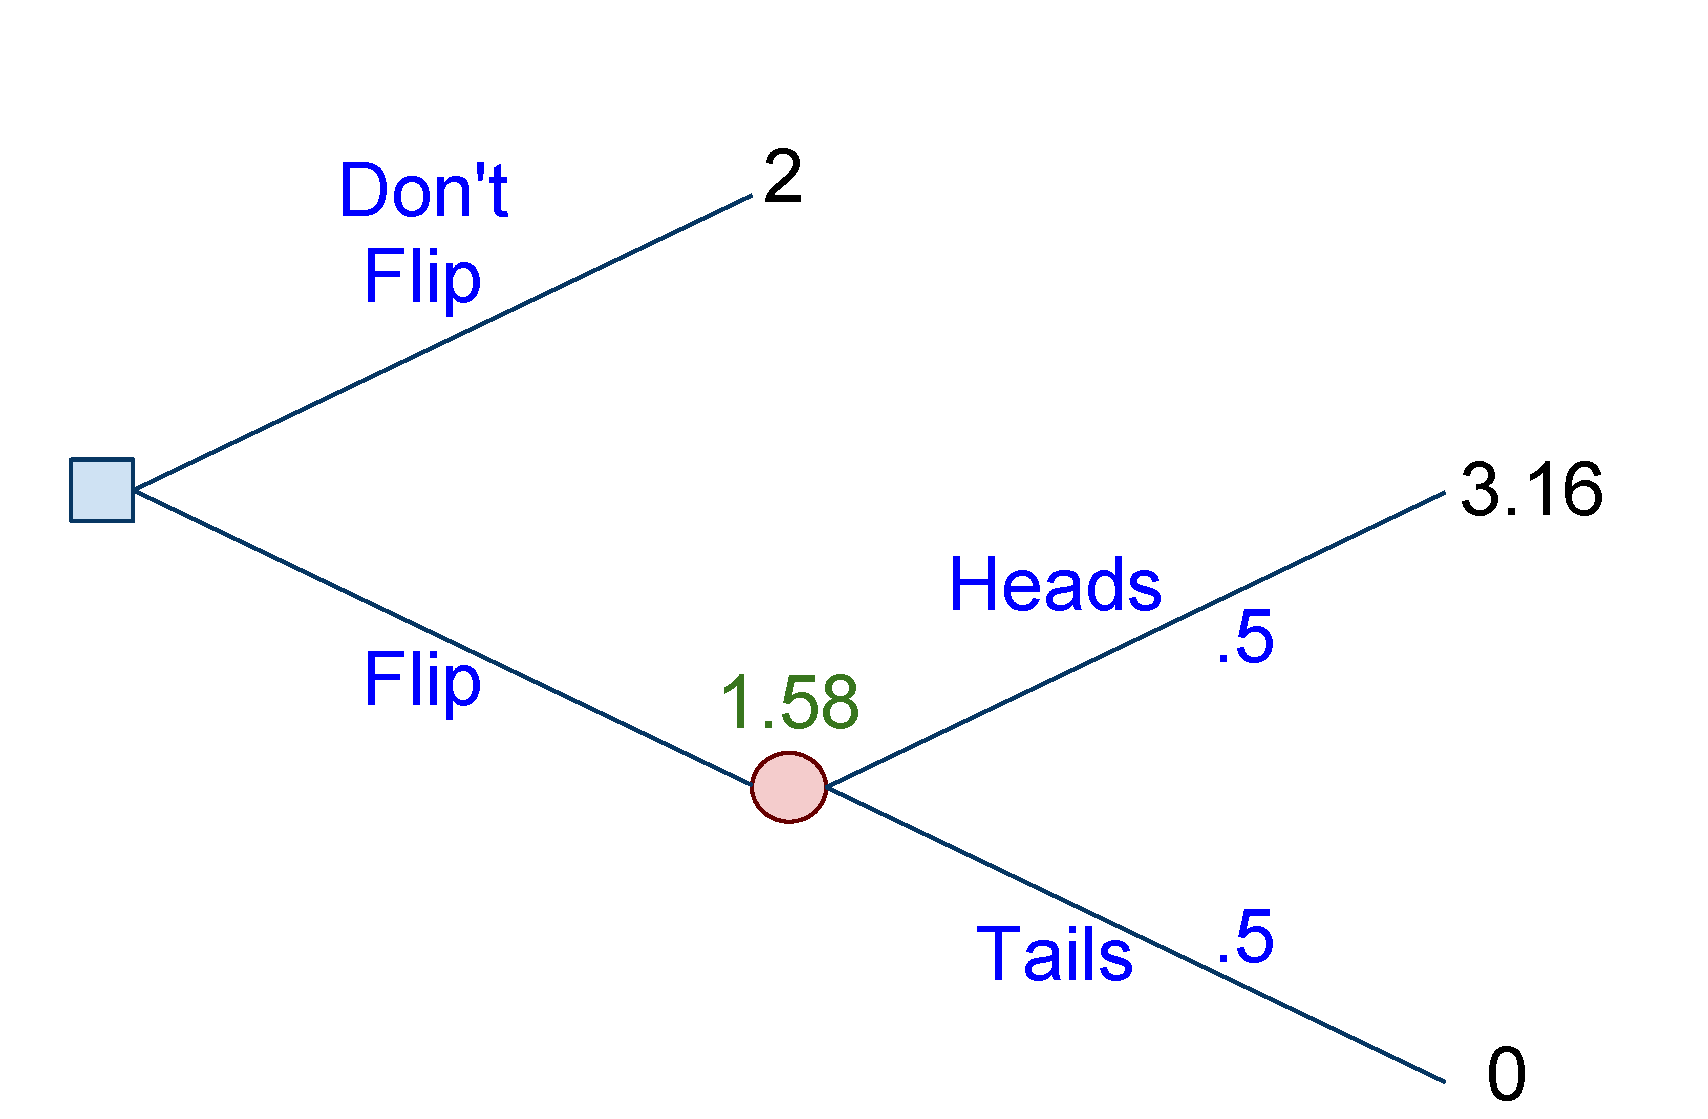
\includegraphics[width=7cm]{Coin_Flip_with_utility_3.pdf}
\end{center}}}

\frame{\frametitle{Utility Functions}
3 categories of utility functions:
\begin{itemize}
\item \textbf{Risk-averse}: the utility function is risk-averse if it is concave:
$$u(x)=\sqrt{x}$$
\item \textbf{Risk-seeking}: the utility function is risk-seeking if it is convex:
$$u(x)=x^2$$
\item \textbf{Risk-neutral}: the utility function is risk-neutral if is is linear:
$$u(x)=x$$
\end{itemize}}

\frame{\frametitle{Utility Functions}
\begin{center}
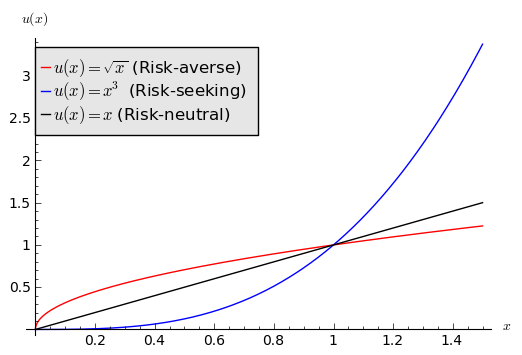
\includegraphics[width=10cm]{utility}
\end{center}}

\frame{\frametitle{Choice of utility function}
When a utility function is used for decision analysis, the utility function must be constructed to fit the preferences and values of the decision maker.
}

\frame{\frametitle{Munduruku Example}In ``Alex's Adventures in Numberland'' by \textbf{Alex Bellos} an account of the \textbf{Munduruku} tribe is given.
\begin{itemize}
\item Indigenous tribe of 7000.
\item Brazilian Amazon.
\item Language:
	\begin{itemize}
	\item No tense.
	\item No plurals.
	\item No words for numbers $>5$.
	\end{itemize}
\end{itemize}}

\frame{\frametitle{Numerical Experiment}
\begin{center}
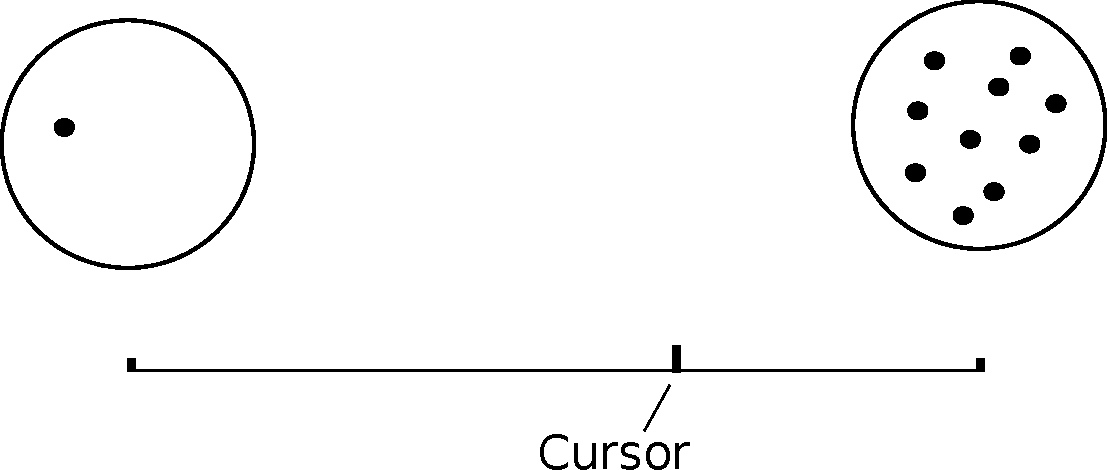
\includegraphics[width=7cm]{munduruku_experiment}
\end{center}
}

\frame{\frametitle{Results}
\begin{center}
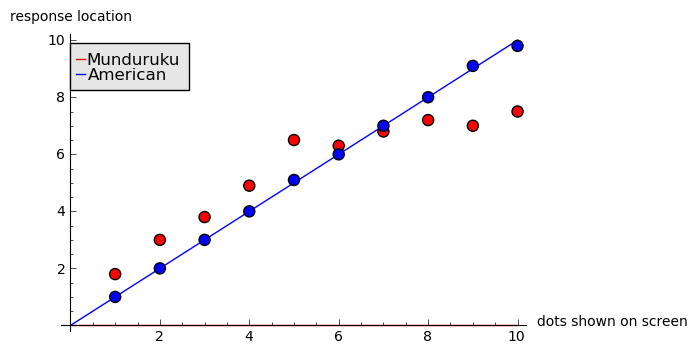
\includegraphics[width=11cm]{experiment_results}
\end{center}}





%
%%\section{Game Theory}
%%
%%\frame{\frametitle{Game Theory: Introduction}
%%Often decision analysis does not only depend on chance but on the decisions made by others: \emph{interactive decision problems}.\\\vspace{.5cm}
%%Such decision problems are called \emph{games}. The individuals making the decisions are called \emph{players}.}
%%
%%\frame{\frametitle{2 Player Static Games}
%%We shall consider 2 player static games. Assume two players have two sets of available strategies: $S_1=\{r_1,\dots,r_m\}$ and $S_2=\{s_1,\dots,s_n\}$. Let $u_1(r,s),\; u_2(r,s)$ be the utility gained by player 1 and 2 for a pair of strategies $(s,r)$. \pause
%%$$\begin{tabular}{|c|c|c|c|c|}
%%\hline
%% &$s_1$      &$s_2$   &\dots&$s_n$  \\\hline
%%$r_1$&$(u_1,u_2)$&$(u_1,u_2)$&\dots&$(u_1,u_2)$\\\hline
%%$r_2$&$(u_1,u_2)$&$(u_1,u_2)$&\dots&$(u_1,u_2)$\\\hline
%%$\vdots$&$\vdots$&$\vdots$&$\ddots$&$\vdots$\\\hline
%%$r_m$&$(u_1,u_2)$&$(u_1,u_2)$&\dots&$(u_1,u_2)$\\\hline
%%\end{tabular}$$\pause
%%Both players aim to choose from their available strategies so as to maximise $u_1$ and $u_2$.
%%}
%%
%%\frame{\frametitle{Example: Prisoner's Dilemma}
%%Two criminal suspects have been caught. They have been isolated and are being questioned separately by the police. The following offer is made to both suspects:
%%\begin{itemize}
%%\item If one confesses that they both committed the crime then the confessor will be set free and the other will spend 5 years in jail.
%%\item If both confess, then they will each get a 4 year sentence.
%%\item If neither confess, then they will each spend 2 years in jail.
%%\end{itemize}
%%}
%%
%%\frame{\frametitle{Example: Prisoner's Dilemma}
%%Both \emph{players} have 2 possible strategies:\begin{itemize}
%%\item Keep quite (Q)
%%\item Squeal (S)
%%\end{itemize}
%%\pause
%%
%%
%%%\psgrid(3,0)(7,5)
%%$$\begin{tabular}{|c|c|c|}
%%\hline
%% &$Q$      &$S$     \\\hline
%%$Q$&(-2,-2)&(-5,0)\\\hline
%%$S$&(0,-5)&(-4,-4)\\\hline
%%\end{tabular}$$\pause
%%
%%The solution of the game is $(S,S)$. Both criminals squeal and go to prison for 4 years (Instead of 2).
%%
%%}
%%
%%\frame{\frametitle{Solving games using Dominance}
%%We solved the prisoners' dilemma in an intuitively simple manner by observing the strategy $S$ was always better then $Q$. We attempt to solve games by eliminating poor strategies for each player.\\\vspace{.5cm}
%%\begin{itemize}\item A strategy for player 1, $r_i$ is, \emph{strictly dominated} by $r_j$ if
%%$$u_1(r_i,s)< u_1(r_j,s) \text{ for all }s\in S_2$$
%%\item A strategy for player 1, $r_i$ is, \emph{weakly dominated} by $r_j$ if
%%$$u_1(r_i,s_k)\leq u_1(r_j,s_k) \text{ for all }s_k\in S_2$$
%%and there exists a strategy $s_l\in S_2$ such that:
%%$$u_1(r_i,s_l)< u_1(r_j,s_l)$$
%%\end{itemize}}
%%
%%\frame{\frametitle{Example}
%%Consider the following game:
%%\begin{center}\pspicture(0,2)(0,4)
%%\rput[b](0,2){$\begin{tabular}{|c|c|c|}
%%\hline
%% &$s_1$      &$s_2$     \\\hline
%%$r_1$&$(3,3)$&$(2,2)$\\\hline
%%$r_2$&$(2,1)$&$(2,1)$\\\hline
%%\end{tabular}$}
%%\only<2>{\psline[linecolor=red,linearc=.2](1,3.75)(1,1.75)}
%%\only<3>{
%%\psline[linecolor=red,linearc=.2](1,3.75)(1,1.75)
%%\psline[linecolor=red,linearc=.2](-2,2.25)(2,2.25)}
%%\endpspicture\end{center}
%%
%%
%%For player 2, $s_1$ weakly dominates $s_2$. For player 1, $r_1$ weakly dominates $r_2$. Thus $(s_1,r_1)$ is the solution of this game.
%%}
%%
%%\frame{\frametitle{Common Knowledge of Rationality}
%%To solve a game by the elimination of dominated strategies we have to assume that the players are rational. However, we can go further, if we also assume that:
%%\begin{itemize}
%%\item The players are rational.\pause
%%\item The players all know that the other players are rational.\pause
%%\item The players all know that the other players know that they are rational.\pause
%%\item \dots
%%\end{itemize}
%%This chain of assumptions is call \emph{Common Knowledge of Rationality} (CKR). By applying the CKR assumption, we can solve a game by iterating the elimination of dominated strategies.}
%%
%%\frame{\frametitle{Example}
%%\begin{center}\pspicture(0,2)(0,4)
%%\rput[b](0,2){$\begin{tabular}{|c|c|c|c|}
%%\hline
%% &$s_1$      &$s_2$  &$s_3$   \\\hline
%%$r_1$&$(1,0)$&$(1,2)$&$(0,1)$\\\hline
%%$r_2$&$(0,3)$&$(0,1)$&$(2,0)$\\\hline
%%\end{tabular}$}
%%\only<2>{\psline[linecolor=red,linearc=.2](1.65,3.75)(1.65,1.75)}
%%\only<3>{
%%\psline[linecolor=red,linearc=.2](1.65,3.75)(1.65,1.75)
%%\psline[linecolor=red,linearc=.2](-2.5,2.25)(2.5,2.25)}
%%\only<4>{
%%\psline[linecolor=red,linearc=.2](1.65,3.75)(1.65,1.75)
%%\psline[linecolor=red,linearc=.2](-2.5,2.25)(2.5,2.25)
%%\psline[linecolor=red,linearc=.2](-.9,3.75)(-.9,1.75)}
%%\endpspicture\end{center}
%%\textbf{Initially} player 1 has no dominated strategies. For player 2, $s_3$ is dominated by $s_2$. \textbf{Now}, $r_2$ is dominated by $r_1$. \textbf{Finally}, $s_1$ is dominated by $s_2$. Thus $(s_1,r_1)$ is the solution of this game.
%%}
%%
%%\frame{\frametitle{Nash Equilibrium}
%%Importantly, certain games cannot be solved using the iterated elimination of dominated strategies:
%%$$\begin{array}{c@{\hspace{1cm}}c}
%%\begin{tabular}{|c|c|c|c|}
%%\hline
%% &$s_1$      &$s_2$  &$s_3$   \\\hline
%%$r_1$&$(10,0)$&$(5,1)$&$(4,-2)$\\\hline
%%$r_2$&$(10,1)$&$(5,0)$&$(1,-1)$\\\hline
%%\end{tabular}
%%&
%%\begin{tabular}{|c|c|c|c|}
%%\hline
%% &$s_1$      &$s_2$  &$s_3$   \\\hline
%%$r_1$&$(1,3)$&$(4,2)$&$(2,2)$\\\hline
%%$r_2$&$(4,0)$&$(0,3)$&$(4,1)$\\\hline
%%$r_3$&$(2,5)$&$(3,4)$&$(5,6)$\\\hline
%%\end{tabular}
%%\end{array}$$\pause
%%(exercise: why does iterated elimination fail here?)
%%}
%%
%%\frame{\frametitle{Nash Equilibrium}
%%A \emph{Nash equilibrium} is a pair of strategies $(\tilde r,\tilde s)$ such that
%%$$u_1(\tilde r,\tilde s)\geq u_1(r,\tilde s)\text{ for all }r\in S_1$$
%%and
%%$$u_1(\tilde r,\tilde s)\geq u_1(\tilde r, s)\text{ for all }s\in S_2$$}
%%
%%\frame{\frametitle{Testing for Nash Equilibrium}
%%One can find Nash equilibrium by checking all strategy pairs and seeing if either player can improve their outcome.
%%\begin{center}\pspicture(0,-1)(0,1)
%%%\psgrid(-5,-3)(5,5)
%%\rput(0,0){\begin{tabular}{|c|c|c|c|}
%%\hline
%% &$s_1$      &$s_2$  &$s_3$   \\\hline
%%$r_1$&$(10,0)$&$(5,1)$&$(4,-2)$\\\hline
%%$r_2$&$(10,1)$&$(5,0)$&$(1,-1)$\\\hline
%%\end{tabular}}
%%\pause
%%\pspolygon[linecolor=blue](-1.65,-.75)(-.45,-.75)(-.45,-.25)(-1.65,-.25)
%%\pause
%%\pspolygon[linecolor=blue](-.2,.25)(.8,.25)(.8,-.25)(-.2,-.25)
%%\endpspicture
%%\end{center}
%%\pause
%%Nash Equilibria need not be unique!
%%}

\end{document}
